\PassOptionsToPackage{dvipsnames,svgnames,table}{xcolor}
\documentclass[11pt]{article}
\usepackage[a4paper,margin=22mm]{geometry}
\usepackage[no-math]{fontspec}
\setmainfont{DejaVu Serif}
\usepackage{amsmath,amssymb,amsthm,mathtools,graphicx,xcolor,hyperref,xurl,xspace,ifthen,enumerate}
\usepackage[shortlabels]{enumitem}
\setlength{\emergencystretch}{4em}
\AtBeginDocument{\special{pdf:mapline pzdr Dingbats <uzdr.pfb}}
\SetMathAlphabet{\mathbf}{normal}{OT1}{cmr}{bx}{n}
\SetMathAlphabet{\mathbf}{bold}{OT1}{cmr}{bx}{n}
\newtheorem{theo}{Theorem}[section]
\newtheorem{lemm}[theo]{Lemma}
\newtheorem{thm}[theo]{Theorem}
\newtheorem{proposition}[theo]{Proposition}
\newtheorem{corollary}[theo]{Corollary}
\newtheorem{definition}[theo]{Definition}
\newtheorem{theorem}[theo]{Theorem}
\newtheorem*{remas*}{Remarks}
\newtheorem{remas}[theo]{Remarks}
\newtheorem*{exam*}{Example}
\newtheorem{ques}[theo]{Question}
\providecommand{\og}{«\nobreakspace}
\providecommand{\fg}{\nobreakspace»}
\newtheorem{lem}[theo]{Lemma}
\newtheorem{lemma}[theo]{Lemma}
\newtheorem{prop}[theo]{Proposition}
\newtheorem{coro}[theo]{Corollary}
\newtheorem{corol}[theo]{Corollary}
\newtheorem*{conj*}{Conjecture}
\newtheorem{conj}[theo]{Conjecture}
\newtheorem{conjecture}[theo]{Conjecture}
\newtheorem{Proposition}[theo]{Proposition}
\newtheorem{theoreme}[theo]{Theorem}
\theoremstyle{definition}
\newtheorem{defi}[theo]{Definition}
\newtheorem{exam}[theo]{Example}
\newtheorem{exem}[theo]{Example}
\newtheorem{remark}[theo]{Remark}
\newtheorem{example}[theo]{Example}
\newtheorem{rema}[theo]{Remark}
\newtheorem{nota}[theo]{Notation}
\newtheorem{notation}[theo]{Notation}
\newtheorem{question}[theo]{Question}
\newtheorem{prob}[theo]{Problem}
\newtheorem*{rema*}{Remark}
\newtheorem*{defi*}{Definition}
\newtheorem*{theo*}{Theorem}
\newtheorem*{lemm*}{Lemma}
\newtheorem*{prop*}{Proposition}
\newcommand{\enoncename}{}
\newtheorem{corpusenonce}[theo]{\enoncename}
\newenvironment{enonce}[2][]{\renewcommand{\enoncename}{#2}\begin{corpusenonce}}{\end{corpusenonce}}
\newenvironment{enonce*}[2][]{\par\medskip\noindent\textbf{#2.}\itshape}{\par\medskip}
\newenvironment{proofc}[1][\proofname]{\begin{proof}[#1]}{\end{proof}}
\newcommand{\Mc}{\mathcal{M}}
\newcommand{\pointir}{.\ ---\ }
\newcommand{\equalenv}[2]{\expandafter\let\csname#1\expandafter\endcsname\csname#2\endcsname\expandafter\let\csname end#1\expandafter\endcsname\csname end#2\endcsname}
\providecommand{\diagbox}[3][]{\begin{tikzpicture}[x=1em,y=1em,baseline=(current bounding box.center)]\useasboundingbox(0,0) rectangle(3,1.4);\draw(0,1.4)--(3,0);\node at(.5,.3){#2};\node at(2.5,1.1){#3};\end{tikzpicture}}
\providecommand{\eg}{e.g.\ }
\providecommand{\ie}{i.e.\ }
\providecommand{\cf}{cf.\ }

\providecommand{\mathof}[1]{\mathrm{#1}}

\numberwithin{equation}{section}


\def\endappendix{}


\usepackage{tabularx}
\newcommand{\iddots}{\mathinner{\mkern1mu\raise1pt\hbox{.}\mkern2mu\raise4pt\hbox{.}\mkern2mu\raise7pt\hbox{.}\mkern1mu}}
\usepackage{mathrsfs}
\usepackage{graphicx}
% Unused ytableau import omitted; no tableau macro occurs in retained native body.
\usepackage{tikz}
\usetikzlibrary{arrows}
\usetikzlibrary{arrows.meta}
\tikzset{>={Latex[width=1.2mm,length=1.7mm]}}

\usepackage[matrix,arrow,tips,curve]{xy}
      






  


\begin{document}
\section*{\raggedright 775: Type-BC zig-zag networks classify 3412- and 4231-avoiding hyperoctahedral permutations}
\noindent\textbf{Author:} Skandera, Mark A.\par\noindent\textbf{Source:} Hyperoctahedral group characters and a type-BC analog of graph coloring. Algebraic Combinatorics 8 (2025), publisher version, DOI 10.5802/alco.459. \url{https://alco.centre-mersenne.org/articles/10.5802/alco.459/}
\par\noindent\textbf{License:} CC BY 4.0, \url{https://creativecommons.org/licenses/by/4.0/}. The original publisher PDF cover has the explicit license notice. See the saved source/license records.
\par\noindent\textbf{Editorial material note (not author text):} The selected problem is Theorem5.18: the authored type-BC zig-zag networks correspond bijectively to hyperoctahedral permutations avoiding unsigned3412/4231. All Section5 native definitions/interval factorization diagrams, direct-sum proof and both classification directions are retained, along with required earlier permutation/pattern and network conventions. Two unselected standard-Bruhat numerical tableau illustrations at source725--733 and739--747 are omitted; their standard definitions/cited facts and adjacent proof remain intact. Later Sections6--12 character/tableau/graph-coloring results are unselected, with introductory references preserved as exact original printed locators. Original graph figures remain bounded figure-only vector assets, and all mathematical prose/formulas/new proof construction remains editable native TeX. Named prior type-A network/pattern results remain explicit prerequisites. All proof text and formulas below are editable author TeX. Mathematical wording, language and proof order are retained. Only the article class, title matter and bibliography presentation are adapted for independent compilation; no proof has been generated or repaired.
\par\noindent\textbf{Editorial difficulty:} H2: The proof controls mirrored interval factors and signed reversal factorizations, then inducts on decomposable and indecomposable skew-symmetric permutations to obtain the exact type-BC network class. The explicit factorization argument is a nonroutine structural classification with both pattern restrictions preserved.
\medskip\hrule\medskip
\noindent\textbf{Author statement, complete proof and local supporting text follow in source order.}
\newtheorem{alg}[theo]{Algorithm}
\equalenv{lem}{lemm}
\equalenv{cor}{coro}
\equalenv{defn}{defi}

\newcommand{\sn}{\mathfrak{S}_n}
\newcommand{\sr}{\mathfrak{S}_r}
\newcommand{\mfs}[1]{\mathfrak{S}_{#1}}
\newcommand{\snn}{\mfs{\smash{[\ol n, n]}}}
\newcommand{\mfsmin}[1]{\mathfrak{S}_-^{#1}}
\newcommand{\bn}{\mathfrak{B}_n}
\newcommand{\br}{\mathfrak{B}_r}
\newcommand{\mfb}[1]{\mathfrak{B}_{#1}}
\newcommand{\mfbmin}[1]{\mathfrak{B}_-^{#1}}
\newcommand{\zsn}{\mathbb{Z}[\sn]}
\newcommand{\qsn}{\mathbb{Q}[\sn]}
\newcommand{\zbn}{\mathbb{Z}[\bn]}
\newcommand{\qbn}{\mathbb{Q}[\bn]}
\newcommand{\cx}{\mathbb{C}[x]}
\newcommand{\zx}{\mathbb{Z}[x]}
\newcommand{\cxn}{\mathbb{C}[x_{1,1},\dotsc,x_{n,n}]}
\newcommand{\zxn}{\mathbb{Z}[x_{1,1},\dotsc,x_{n,n}]}
\newcommand{\zqq}{\mathbb{Z}[q, q^{-1}]}
\newcommand{\csn}{\mathbb{C}[\sn]}
\newcommand{\bitab}{\mathcal B}
\newcommand{\tab}{\mathcal U}
\newcommand{\bctab}{\mathcal U^{\msfBC}}
\newcommand{\atab}{\mathcal U^{\msfA}}
\newcommand{\ol}[1]{\overline{#1}}

\newcommand{\hnq}{H_n(q)}
\newcommand{\hbnq}{H_n^{\msfBC}(q)}
\newcommand{\hbq}[1]{H_{#1}^{\msfBC}(q)}
\newcommand{\hrq}{H_r(q)}
\newcommand{\hlq}{H_\lambda(q)}
\newcommand{\A}{\mathcal{A}}
\newcommand{\anq}{\mathcal{A}(n,q)}
\newcommand{\atwonq}{\mathcal{A}(2n,q)}
\newcommand{\arq}{\mathcal{A}(r;q)}
\newcommand{\arnq}{\mathcal{A}_r}
\newcommand{\annq}{\mathcal{A}_n(n;q)}
\newcommand{\Ann}{\mathcal{A}_{[n],[n]}}
\newcommand{\trsp}{\mathcal{T}}
\newcommand{\btrsp}{\mathcal{T}^{BC}}

\newcommand{\coh}{\mathrm{H}}
\newcommand{\icoh}{\mathrm{IH}}
\newcommand{\HH}{\mathcal{H}}

\newcommand{\redexp}[2]{s_{i_{#1}} \ntnsp \cdots s_{i_{#2}}}
\newcommand{\wtc}[2]{\widetilde{C}_{#1}(#2)}
\newcommand{\btc}[2]{\widetilde{C}_{#1}^{\msfBC}(#2)}

\newcommand{\imm}[1]{\mathrm{Imm}_{#1}}
\newcommand{\bnimm}[1]{\mathrm{Imm}_{#1}^{\bn}}
\newcommand{\simm}[2]{\mathrm{Imm}_{#2}^{\smash{\mfs{#1}}}}

\newcommand{\sumsb}[1]{\sum_{\substack{#1}}}  %%%for multi-line sums
\newcommand{\prodsb}[1]{\prod_{\substack{#1}}}  %%%for multi-line products
\newcommand{\inv}{\textsc{inv}}
\newcommand{\rinv}{\textsc{rinv}}
\newcommand{\defeq}{:=} 
\newcommand{\dfct}{\mathrm{dfct}}
\newcommand{\dnc}{\textsc{dnc}}
\newcommand{\dc}{\textsc{dc}}
\newcommand{\pnc}{\textsc{pnc}}
\newcommand{\sct}{\mathrm{sct}}
\newcommand{\des}{\mathrm{des}}
\newcommand{\exc}{\mathrm{exc}}
\newcommand{\stat}{\mathrm{stat}}
\newcommand{\frobch}{\mathrm{ch}}
\newcommand{\npfrobch}{\mathrm{nch}}
\newcommand{\pfrobch}{\mathrm{pch}}
\newcommand{\spn}{\mathrm{span}}
\newcommand{\sgn}{\mathrm{sgn}}
\newcommand{\triv}{\mathrm{triv}}
\newcommand{\wgt}{\mathrm{wgt}}
\newcommand{\src}{\mathrm{src}}
\newcommand{\snk}{\mathrm{snk}}
\newcommand{\type}{\mathrm{type}}
\newcommand{\ctype}{\mathrm{ctype}}
\newcommand{\inc}{\mathrm{inc}}
\newcommand{\ngr}{\mathrm{ngr}}
\newcommand{\incross}{\textsc{invnc}}
\newcommand{\cdncross}{\textsc{cdnc}}
\newcommand{\cross}{\textsc{c}}
\newcommand{\pavoiding}{$3412$-avoiding, $4231$-avoiding }
\newcommand{\avoidsp}{avoids the patterns $3412$ and $4231${}}
\newcommand{\avoidp}{avoid the patterns $3412$ and $4231${}}
\newcommand{\avoidingp}{avoiding the patterns $3412$ and $4231${}}
\newcommand{\theps}{the patterns $3412$ and $4231${}}
\newcommand{\avoidsignedp}{avoid the signed patterns $1\ol2$, $\ol21$, $\ol2\ol1$, $312$, $3\ol12${}}
\newcommand{\avoidssignedp}{avoids the signed patterns $1\ol2$,  $\ol21$, $\ol2\ol1$, $312$, $3\ol12${}}
\newcommand{\avoidingsignedp}{avoiding the signed patterns $1\ol2$, $\ol21$, $\ol2\ol1$, $312$, $3\ol12${}}
\newcommand{\ul}[1]{\underline{#1}}  
\newcommand{\ssec}[1]{\subsection{#1}{$\negthinspace$}}

\newcommand{\tr}{{\negthickspace \top \negthickspace}}
\newcommand{\nhtnsp}{\kern-0.08333em}
\newcommand{\ntnsp}{\negthinspace}
\newcommand{\ntksp}{\negthickspace}
\newcommand{\nTksp}{\negthickspace\negthickspace}
\newcommand{\nTknsp}{\negthickspace\negthickspace\negthinspace}
\newcommand{\nTtksp}{\negthickspace\negthickspace\negthickspace}
\newcommand{\nTTksp}{\negthickspace\negthickspace\negthickspace
	\negthickspace}
\newcommand{\nTTtksp}{\negthickspace\negthickspace\negthickspace
	\negthickspace\negthickspace}

\newcommand{\oglnc}{{\mathcal O}(\mathrm{GL}_n (\mathbb C))}
\newcommand{\oqglnc}{{\mathcal O}_q(\mathrm{GL}_n (\mathbb C))}
\newcommand{\oslnc}{{\mathcal O}(\mathrm{SL}_n) (\mathbb C)}
\newcommand{\oslthreec}{{\mathcal O}(\mathrm{SL}_3 (\mathbb C))}
\newcommand{\oqslnc}{{\mathcal O}_q(\mathrm{SL}_n (\mathbb C))}
\newcommand{\ospnc}{{\mathcal O}(\mathrm{SP}_{2n} (\mathbb C))}
\newcommand{\oqspnc}{{\mathcal O}_q(\mathrm{SP}_{2n} (\mathbb C))}
\newcommand{\uglnc}{U(\mathfrak{gl}(n,\mathbb{C}))}
\newcommand{\uqglnc}{U_q(\mathfrak{gl}(n,\mathbb{C}))}
\newcommand{\uslnc}{U(\mathfrak{sl}(n,\mathbb{C}))}
\newcommand{\uqslnc}{U_q(\mathfrak{sl}(n,\mathbb{C}))}
\newcommand{\uspnc}{U(\mathfrak{sp}_{2n}(\mathbb{C}))}
\newcommand{\uqspnc}{U_q(\mathfrak{sp}_{2n}(\mathbb{C}))}
\newcommand{\mat}[1]{\mathrm{Mat}_{#1 \times #1}}
\newcommand{\spc}[1]{\mathfrak{sp}_{#1}(\mathbb{C})}
\newcommand{\slc}[1]{\mathfrak{sl}_{#1}(\mathbb{C})}
\newcommand{\fl}[1]{\mathcal{F}_{#1}}
\newcommand{\PiBC}{\Pi^{\msfBC}}


\newcommand{\qdet}{\mathrm{det}_q}
\newcommand{\qper}{\mathrm{per}_q}
\newcommand{\perm}{\mathrm{per}}
\newcommand{\rnk}{\mathrm{rank}}
\newcommand{\sort}{\mathrm{sort}}
\newcommand{\diag}{\mathrm{diag}}
\newcommand{\shape}{\mathrm{shape}}
\newcommand{\hess}{\mathrm{Hess}}
\newcommand{\ahess}{\mathrm{Hess^{\msfA}}}
\newcommand{\bhess}{\mathrm{Hess}^{\msfBB}}
\newcommand{\chess}{\mathrm{Hess}^{\msfC}}
\newcommand{\permmon}[2]{#1_{1,#2_1} \ntnsp\cdots #1_{n,#2_n}}
\newcommand{\bpermmon}[2]
           {#1_{\smash{\ol n,#2_{\ol n}}} \ntnsp\cdots #1_{\smash{\ol 1,#2_{\ol 1}}}
           #1_{1,#2_{1}} \ntnsp\cdots #1_{n,#2_n} }
\newcommand{\sprod}[2]{s_{#1_1} \ntnsp\cdots s_{#1_#2}}
\newcommand{\sintprod}[3]{s_{[#1_1,#2_1]} \ntnsp\cdots s_{[#1_#3, #2_#3]}}
\newcommand{\ssm}{\smallsetminus}
\newcommand{\multiu}{\Cup}
\newcommand{\bs}{\backslash}  
\newcommand{\bfx}{\mathbf x}
\newcommand{\wleq}{\leq_W}
\newcommand{\wless}{<_W}  
\newcommand{\slambda}{\mathfrak{S}_\lambda}
\newcommand{\slambdamin}{\mathfrak{S}_\lambda^{-}}
\newcommand{\phmin}{\phantom{-}}
\newcommand{\circd}[1]{\raisebox{-9pt}{\textcircled{\raisebox{-.9pt}{#1}}}}
\newcommand{\sdot}{\left[ \begin{smallmatrix} 0 & -1 \\ 1 & \phantom{-}0 \end{smallmatrix}\right]}
\newcommand{\sddot}{\left[ \begin{smallmatrix} \phantom{-}0 & 1 \\ -1 & 0 \end{smallmatrix}\right]}
\newcommand{\sreg}{\left[ \begin{smallmatrix} 0 & 1 \\ 1 & 0 \end{smallmatrix}\right]}
\newcommand{\smallj}{\left[ \begin{smallmatrix} 0 & \phantom{\int} & 1 \\ & \smash{\iddots} & \phantom{T} \\ 1 & & 0 \end{smallmatrix}\right]}
\newcommand{\abdiag}[1]{\left[ \begin{smallmatrix} 1 & #1 \\ 0 & 1 \end{smallmatrix}\right]}
\newcommand{\bediag}[1]{\left[ \begin{smallmatrix} 1 & 0 \\ #1 & 1 \end{smallmatrix}\right]}
\newcommand{\upparrow}{\big \uparrow \nTksp \phantom{\uparrow}}
\newcommand{\upparrowa}{\big \uparrow \ntksp \phantom{\uparrow}}
\newcommand{\precdot}{\prec \negthickspace \negthinspace \cdot\ }
\newcommand{\net}[2]{\mathcal F^{\mathsf{#1}}(#2)}
\newcommand{\snet}[2]{\mathcal S^{\mathsf{#1}}(#2)}
\newcommand{\znet}[2]{\mathcal S^{\mathsf{#1}}_{\mathrm Z}(#2)}
\newcommand{\dnet}[2]{\mathcal S^{\mathsf{#1}}_{\mathrm D}(#2)}
\newcommand{\sfA}{\textsf{A}}
\newcommand{\msfA}{\mathsf{A}}
\newcommand{\sfBB}{\textsf{B}}
\newcommand{\msfBB}{\mathsf{B}}
\newcommand{\sfC}{\textsf{C}}
\newcommand{\msfC}{\mathsf{C}}
\newcommand{\sfBC}{\textsf{BC}}
\newcommand{\msfBC}{\mathsf{BC}}
\newcommand{\YBCq}{Y_q^\mathsf{BC}}
\newcommand{\vertex}[1]{#1}
\newcommand{\phsum}{\phantom{\sum_A^Z}}
\newcommand{\phm}{\phantom M}
\newcommand{\phn}{\phantom{ni}}
\newcommand{\bcao}[1]{\mathcal{O}^{\msfBC}({#1})}
\newcommand{\schub}[1]{\Omega_{#1}}
\newcommand{\Aschub}[1]{\Omega_{#1}^{\msfA}}
\newcommand{\Bschub}[1]{\Omega_{#1}^{\msfBB}}
\newcommand{\Cschub}[1]{\Omega_{#1}^{\msfC}}
\newcommand{\tripprox}{\setbox0\hbox{$\approx$}%
\mbox{\makebox[0pt][l]{\raisebox{0.48\ht0}{$\approx$}}$\approx$}}
\newcommand*{\diffeo}{% 
  \mathrel{\vcenter{\offinterlineskip
  \hbox{$\sim$}\vskip-.35ex\hbox{$\sim$}\vskip-.35ex\hbox{$\sim$}}}}

\theoremstyle{remark}

\section{Introduction}\label{s:intro}

Let $W$ be a Coxeter group, $H = H(W)$ its Hecke algebra, and $\trsp(H)$ the
space of Hecke algebra {\em traces},
linear functionals $\theta_q: H \rightarrow \zqq$ satisfying
$\theta_q(DD') = \theta_q(D'D)$ for all $D, D' \in H$.
Included in $\trsp(H)$ are the $H$-characters,
which encode much of the structure of $H$ in a condensed form.
Since traces are linear,
one might hope to solve the
following problem for particular bases
$\mathcal D = \{ D_w \,|\, w \in W \}$ of $H$
and $\Theta = \{ \theta_q^{(i)} \,|\, i = 1,\dotsc,p \}$
of $\trsp(H)$.
\begin{prob}\label{p:evaltrace}
  Find combinatorial formulas for
  each of the trace evaluations
$\{ \theta_q^{(i)} (D_w) \,|\,
\theta_q^{(i)} \ntnsp\in \Theta, D_w \ntnsp\in \mathcal D\}$.
\end{prob}

Unfortunately, trace evaluation is not always easy,
even in type $\msfA$,
when $W$ is the symmetric group $\sn$ with Hecke algebra $H = \hnq$.
(See e.g. \cite[\S 1]{CHSSkanEKL}.)
Type-$\msfA$ solutions were given in
\cite{CSkanTNNChar, KLSBasesQMBIndSgn},
using the induced sign character basis of $\trsp(\hnq)$,
and bases consisting of products of simple elements of
the (modified, signless) Kazhdan--Lusztig basis
$\{ \wtc wq \,|\, w \in \sn \}$ of $\hnq$.
It would be interesting to solve Problem~\ref{p:evaltrace}
for other pairs of type-$\msfA$ bases as well, as these evaluations are related to
facts and conjectures
concerning nonnegativity,
graph coloring, and Hessenberg varieties. (See e.g.
\cite[Lem.\,1.1]{HaimanHecke},
\cite[Conj.\,2.1]{HaimanHecke},  
\cite[Conj.\,4.9]{SWachsChromQ},
\cite[Conj.\,5.5]{StanStemIJT}.)

Partial type-$\msfA$ solutions to Problem~\ref{p:evaltrace}
were given in \cite{CHSSkanEKL, SkanCCS}
for various bases of $\trsp(\hnq)$, and
the subset
\begin{equation}\label{eq:introsmooth}
  \{ \wtc wq \,|\, w \in \sn \text{ \avoidsp} \}
\end{equation}
of the Kazhdan--Lusztig basis of $\hnq$.
By \cite[Thm.\,4.3]{SkanNNDCB},
we have that for $w$ \avoidingp, there exists a planar network $F = F(w)$
which serves as a combinatorial interpretation for $\wtc wq$.
By \cite[Thm.\,7.4]{CHSSkanEKL},
there also exist
a poset $P = P(w)$
and graph $G = G(w)$
such that
evaluations $\theta_q( \wtc wq )$ may be computed combinatorially
by
\begin{enumerate}
\item filling Young diagrams with paths in $F$,
\item filling Young diagrams with elements of $P$,
\item coloring vertices of $G$, 
\item orienting edges of $G$,
\end{enumerate}
while obeying certain rules in each case.
(See also \cite{AthanPSE, SWachsChromQF, StanSymm}.)
While \eqref{eq:introsmooth} is only a subset of the Kazhdan--Lusztig basis
of $\hnq$, it is conjectured~\cite[Conj.\,1.9]{ANigroUpdate},
\cite[Conj.\.3.1]{HaimanHecke} that an even smaller subset
\begin{equation}\label{eq:introcodom}
  \{ \wtc wq \,|\, w \in \sn
  \text{ is codominant, i.e. avoids the pattern } 312 \}
\end{equation}
explains trace evaluations at the entire Kazhdan--Lusztig basis.
It is known~\cite[Thm.\,4.6]{CHSSkanEKL}
that for each element $\wtc wq$ of \eqref{eq:introsmooth}
there exists an element $\wtc vq$ of \eqref{eq:introcodom}
with the property that $P(w) \cong P(v)$
and therefore that $\theta_q(\wtc wq) = \theta_q(\wtc vq)$ for all traces
$\theta_q \in \trsp(\hnq)$.

One could also answer Problem~\ref{p:evaltrace}
from the point of view of symmetric functions.
Let $\Lambda_n$ be the $\mathbb Z$-module of homogeneous, degree-$n$
symmetric functions.
Since the ranks of $\Lambda_n$ and $\trsp(\hnq)$ are
equal,
it is possible to define
a generating function in $\Lambda_n$
for evaluations of traces at
any fixed element $D \in \hnq$.
Following \cite[\S 2]{SkanCCS},
we use
the induced sign character basis $\{\epsilon_q^\lambda\}$ of $\trsp(\hnq)$
and monomial symmetric function basis $\{ m_\lambda \}$ of $\Lambda_n$
to define
\begin{equation*}
  Y_q(D) \defeq \sum_\lambda
  \epsilon_q^\lambda (D) m_\lambda \in \zqq \otimes \Lambda_n.
\end{equation*}
A certain pairing of six natural bases of $\trsp(\hnq)$
and six natural bases of $\Lambda_n$ then guarantees that for each pair
$(\{ \theta_q^\lambda \}, \{ g_\lambda \})$,
we have
\begin{equation*}
  Y_q(D) = \sum_\lambda \theta_q^\lambda(D) g_\lambda.
\end{equation*}
Thus $Y_q(D)$ is in fact a generating function for the evaluation
of all elements of these six trace bases
at $D$. (See e.g. \cite[Prop.\,2.1]{SkanCCS}.)
Conveniently, the combinatorial computations mentioned above also
guarantee
that a certain
{\em chromatic (quasi-)symmetric function}
$X_{G,q}$, defined in terms of the proper colorings of $G$~\cite{SWachsChromQ},
satisfies $X_{G,q} = Y_q(\wtc wq)$~\cite[Thm.\,7.4]{CHSSkanEKL}.
Thus for $w \in \sn$ \avoidingp,
the graph $G$ essentially encodes all trace evaluations of the
form $\theta_q^\lambda(\wtc wq)$ for $\{ \theta_q^\lambda \}$ one of the six natural
bases of $\trsp(\hnq)$.

Some of the above results
from \cite{CHSSkanEKL, SkanNNDCB, SkanCCS}
have type-$\msfBC$ analogs,
i.e. extensions to the hyperoctahedral group $\bn$
and its Hecke algebra $\hbnq$.
In Sections~\ref{s:s2nbn} -- \ref{s:trace},
we present these algebras, their Kazhdan--Lusztig bases,
and their trace spaces.
In Section~\ref{s:planarnet}, we define type-$\msfBC$ analogs
of type-$\msfA$ planar networks, and use these to
graphically represent the subset
\begin{equation}\label{eq:BCintrosmooth}
  \{ \btc w1 \,|\, w \in \bn \text{ \avoidsp} \}
\end{equation}
of the Kazhdan--Lusztig basis of $\zbn$.
In Section~6 we use immanants and total nonnegativity
to interpret trace evaluations at \eqref{eq:BCintrosmooth}
in terms of paths in the type-$\msfBC$ planar networks. 
In Sections~7 -- 8, we define type-$\msfBC$ analogs
$Q(w)$ and $\Gamma(w)$ of the type-$\msfA$ posets and graphs
associated to planar networks.
We define a type-$\msfBC$ analog of codominant permutations and
show that the posets correspond bijectively to the proper subset
\begin{equation}\label{eq:BCintrocodom}
  \{ \btc w1 \,|\, w \in \bn \text{ $\msfBC$-codominant} \}
\end{equation}
of \eqref{eq:BCintrosmooth}.
We use the above networks, posets, and graphs 
in Section~9
to state and prove our main results on
the combinatorial computation of type-$\msfBC$ trace evaluations,
and in Section~10 to show that
for each element $\btc w1$ of \eqref{eq:BCintrosmooth}
there exists an element $\btc v1$ of \eqref{eq:BCintrocodom}
with the property that $Q(w) \cong Q(v)$
and therefore that $\theta(\btc w1) = \theta(\btc v1)$ for all traces
$\theta \in \trsp(\bn)$.
Formulas in Section~9 lead to natural 
type-$\msfBC$ analogs of
type-$\msfA$ chromatic symmetric functions 
in Section~11.
We finish in Section~12
with open problems concerning Hessenberg varieties.

\section{The symmetric and hyperoctahedral groups}\label{s:s2nbn}

The hyperoctahedral group $\bn$ is closely related to the symmetric
groups on $n$ and $2n$ letters.  To describe these relationships,
we will use 
subintervals of the set
\begin{equation*}
  [\ol n, n] \defeq \{ -n, \dotsc, n \} \ssm \{ 0 \},
  \end{equation*}
where we define
$\ol a = -a$ for all $a \in [\ol n,n]$.
We call any
subset
$[h,l] \defeq \{ h, \dotsc, l \} \ssm \{0 \}$ of $[\ol n,n]$
an {\em interval}, even if $h < 0 < l$.
Let $\mfs{[h,l]}$ denote
the group of permutations of letters in the interval $[h,l]$.
The group $\bn$ is naturally related both to $\snn$
and $\sn = \mfs{[1,n]}$.
To illustrate these relationships and prepare for our main results,
we will consider the groups' presentations, conjugacy classes, Bruhat
orders, and pattern-avoidance definitions.



\ssec{\texorpdfstring{$\bn$}{B\_n} as a subgroup of \texorpdfstring{$\mfs{\smash{[\ol n, n]}}$}{S\_[n-bar, n]}}\label{ss:bnassubgp}
The $2n$th symmetric group
$\mfs{\smash{[\ol n, n]}}$
is the Coxeter group
(see e.g. \cite{BBCoxeter}) of type $\msfA_{2n-1}$,
with generators
  $s_{\ol{n-1}}, \dotsc, s_{\ol 1}, s_0, s_1, \dotsc, s_{n-1}$
and relations
\begin{equation*}
  \begin{alignedat}2
    s_i^2 &= e &\quad &\text{for $i = \ol{n-1}, \dotsc, n-1$,}\\
    s_is_j &= s_js_i &\quad &\text{for $|i-j| \geq 2$,}\\
    s_is_js_i &= s_js_is_j &\quad &\text{for $|i-j| = 1$.}
  \end{alignedat}
\end{equation*}

If an expression $s_{i_1} \cdots s_{i_\ell}$ for $w \in \snn$
is as short as possible,
then call it {\em reduced} and call $\ell = \ell(w)$ the {\em length} of $w$.
Define a (left) action of $\snn$ on rearrangements
$w_{\ol n} \cdots w_{\ol 1} w_1 \cdots w_n$ of the word
$\ol n \cdots \ol 1 1 \cdots n$ by
\begin{equation}\label{eq:laction}
  \begin{cases}
    s_i \text{ swaps letters in positions $i, i+1$}
      &\text{for $i = 1, \dotsc, n-1$},\\
    s_{\ol i} \text{ swaps letters in positions $\ol i, \ol{i+1}$}
      &\text{for $i = 1, \dotsc, n-1$},\\
    s_0 \text{ swaps letters in positions $\ol 1, 1$,}
  \end{cases}
\end{equation}
and
define the {\em one-line notation} of $w = s_{i_1} \cdots s_{i_r} \in \snn$ to be
\begin{equation}\label{eq:s2nrearrange}
  w_{\ol n} \cdots w_{\ol 1} w_1 \cdots w_n 
= s_{i_1}(s_{i_2}( \cdots (s_{i_r}( \ol n \cdots \ol 1 1 \cdots n)) \cdots )).
\end{equation}
For example, when $n=4$, the element $s_{\ol1}s_0s_1$
has one-line notation
\begin{equation*}
    s_{\ol1}(s_0( s_1(\ol4 \ol3 \ol2 \ol1 1234)))
    = s_{\ol1}(s_0(\ol4 \ol3 \ol2 \ol1 2 1 3 4))
    = s_{\ol1}(\ol4 \ol3 \ol2 2 \ol1 1 3 4)
    = \ol4\ol3 2 \ol2 \ol1 1 3 4.
  \end{equation*}
(By our definition, the right action of $s_i$ swaps the letters $i, i+1$,
wherever they are.)
It follows that $w_i^{-1}$ is the index $j$ satisfying $w_j = i$.
It is known that $\ell(w)$ equals the number of {\em inversions} in $w$:
\begin{equation*}
  \inv(w_{\ol n} \cdots w_{\ol1} w_1 \cdots w_n) \defeq
  \{ (j,i) \,|\, j \mkern -2mu > \mkern -2mu i \text{ and $j$ appears before $i$ in $w_{\ol n} \cdots w_{\ol1} w_1 \cdots w_n$} \}.
  \end{equation*}
Thus we have
  $\ell(\ol4\ol32\ol2\ol1134) =
  \inv(\ol4\ol32\ol2\ol1134) =
  |\{(2,\ol2), (2,\ol1), (2,1)\}| = 3$.

For $[a, b] \subseteq [h, l]$
let $\smash{s_{[a,b]}^{[h,l]}}$ be the permutation
in $\mfs{[h,l]}$ whose one-line notation has the form
\begin{equation*}
  h \cdots (a-1) \cdot b (b-1) \cdots (a+1) a \cdot (b+1) \cdots l.
\end{equation*}
When the interval $[h,l]$ is clear from context,
we will simply write $s_{[a,b]}$.
Call such an element a (type-$\msfA$) {\em reversal}.
Observe that the standard generators of $\snn$
are all reversals:
  $s_0 = s_{[-1,1]}$,
  and for $i \geq 1$ we have
  $s_i = s_{[i,i+1]}$,
  $s_{\smash{\ol i}} = s_{\smash{[\ol{i+1},\ol i]}}$. 
Also observe that each trivial reversal $s_{[a,a]}$
is equal to the identity element $e$, and that two reversals $s_{[a,b]}$,
$s_{[c,d]}$ commute
if their intervals $[a,b]$, $[c,d]$ do not intersect.
Let $\bn$ be the Coxeter group of type $\mathsf C_n = \mathsf B_n$,
i.e. the hyperoctahedral group.
We may view $\bn$ as the subgroup of $\snn$
generated by elements
\begin{equation*}
  t\ (\text{also written $s'_0$}) \defeq s_0, \qquad
  s'_i \defeq s_is_{\smash{\ol i}}, \text{ for } i = 1,\dotsc,n-1,
\end{equation*}
which satisfy the relations
\begin{equation*}
  \begin{alignedat}2
    \smash{{s'_i}^2} &= e &\quad &\text{for $i = 0, \dotsc, n-1$,}\\
    ts'_1ts'_1 &= s'_1ts'_1t, &\quad & \\
    s'_is'_j &= s'_js'_i &\quad &\text{for $i,j \geq 0$ and $|i-j| \geq 2$,}\\
    s'_is'_js'_i &= s'_js'_is'_j &\quad &\text{for $i,j \geq 1$ and $|i-j| = 1$.}
  \end{alignedat}
\end{equation*}
The one-line notation for elements of $\bn$ is inherited from that
of $\snn$.
For example, when $n=4$, the element $ts'_1s'_2 \in \mfb4 $
has one-line notation
\begin{equation*}
    t(s'_1(s'_2(\ol4 \ol3 \ol2 \ol1 1234)))
    = ts'_1(\ol4 \ol2 \ol3 \ol1 1 3 2 4))
    = t(\ol4 \ol2 \ol1 \ol3 3 1 2 4)
    = \ol4 \ol2 \ol1 3 \ol3 1 2 4.
  \end{equation*}
If an expression $s'_{i_1} \cdots s'_{i_\ell}$ for $w \in \bn$
is as short as possible,
then call it {\em reduced} and call $\ell = \ell(w)$ the {\em length} of $w$.
Let $\ell_t(w)$ be the number of occurrences of $t$ in any (equivalently, every)
reduced expression for $w$.
Analogously, let $\ell_s(w) = \ell(w) - \ell_t(w)$ be the number
of occurrences of $s'_1,\dotsc,s'_{n-1}$.
It is easy to see that one-line notations of
elements of $\bn$ are precisely the set of
permutations $w_{\ol n} \cdots w_{\ol 1} w_1 \cdots w_n \in \snn$
which satisfy $w_{\ol i} = \ol{w_i}$,
i.e. each is completely determined by the $n$-letter subword
$w_1 \cdots w_n$.
Call these words the {\em long} and
{\em short}
one-line notations of $w$, respectively.
We can read $\ell(w)$, $\ell_t(w)$, $\ell_s(w)$ from the
short one-line notation of $w$ by
\begin{equation*}%\label{eq:ellandellt}
  \ell(w) = \inv(w_1 \cdots w_n) + \sumsb{i > 0\\ w_i < 0} |w_i|,
  \qquad
  \ell_t(w) = \# \{ i > 0 \,|\, w_i < 0 \},
  \end{equation*}
and $\ell_s(w) = \ell(w) - \ell_t(w)$.
Thus we have
  $\ell(\ol3124) = |3| = 3$, $\ell_t(\ol3124) = 1$, and $\ell_s(\ol3124) = 2$.

Define {\em type-$\msfBC$ reversals} to be those elements of $\bn$
having the forms
\begin{equation}\label{eq:creversal}
  \begin{aligned}
    s'_{\smash{[\ol a, a]}} &\defeq s_{\smash{[\ol a, a]}},
        \mbox{ for } 1 \leq a \leq n,\\
    s'_{\smash{[a,b]}} &\defeq s_{\smash{[\ol b, \ol a]}} s_{[a,b]},
    \mbox{ for } 1 \leq a \leq b \leq n,
  \end{aligned}
\end{equation}
where the elements $s_{[a,b]}$ are reversals in $\snn$.

\ssec{Conjugacy classes, partitions, tableaux, bipartitions, bitableaux}\label{ss:conjclasses}
Conjugacy classes of $\sn$ correspond to {\em (integer) partitions} of $n$,
weakly decreasing positive integer sequences
$\lambda = (\lambda_1, \dotsc, \lambda_\ell)$
satisfying $\lambda_1 + \cdots + \lambda_\ell = n$.
The $\ell = \ell(\lambda)$ components of a partition $\lambda$
are called its {\em parts}
and we let the expressions
$|\lambda| = n$ and $\lambda \vdash n$ denote that $\lambda$ is
a partition of $n$.
Sometimes we use the notation $k^{a_k}$ to denote a
sequence of $a_k$ copies of the letter $k$.
Given $\lambda \vdash n$, we define the {\em transpose}
partition $\lambda^\tr = (\lambda_1^\tr, \dotsc,\lambda_{\lambda_1}^{\tr})$ by
$\lambda_i^\tr = \# \{ j \,|\, \lambda_j \geq i \}$. Thus $n^\tr = 1^n$.
We call $\lambda$ {\em self-transpose} if $\lambda^\tr = \lambda$
and we define the empty sequence $\emptyset$ to be the unique partition of the
integer $0$.
Generalizing integer partitions of $n$ are
{\em compositions} $\alpha = (\alpha_1,\dotsc, \alpha_r)$ of $n$,
which are simply positive integer sequences summing to $n$.
We let the notation $\alpha \vDash n$ denote that $\alpha$ is
a composition of $n$. (See e.g. \cite[\S 1.2]{StanEC1}.)

The conjugacy class of $\sn$ corresponding to $\lambda \vdash n$
is the set of all permutations having cycle type $\lambda$.  We write
$\ctype(w) = \lambda$. Letting
$a_k$ be the multiplicity of $k$ in $\lambda$, for $k =1,\dotsc,n$,
we may express the cardinality of the $\lambda$-conjugacy class of $\sn$ as
$n!/z_\lambda$, where
\begin{equation}\label{eq:zlambda}
 z_\lambda = {1^{a_1} \cdots n^{a_n} a_1! \cdots a_n!}.
\end{equation}

Conjugacy classes of $\bn$ correspond to
{\em integer bipartitions of $n$}, pairs $(\lambda,\mu)$
of integer partitions with 
$|\lambda| + |\mu| = n$.
We let
$(\lambda,\mu) \vdash n$ denote that $(\lambda,\mu)$ is
a bipartition of $n$. 
To explicitly describe the conjugacy classes of $\bn$,
we define the homomorphism
\begin{equation}\label{eq:varphi}
  \begin{aligned}
    \varphi: \bn &\rightarrow \sn \\
    s'_i &\mapsto s_i, \quad i=1,\dotsc,n-1,\\
    t &\mapsto e,
  \end{aligned}
  \end{equation}
which replaces letters in the short one-line notation of
$v \in \bn$ by their absolute values.
For each element $v \in \bn$
and each cycle $C = (c_1, \dotsc, c_k = c_0)$
of $\varphi(v) \in \sn$,
define the {\em signed cycle}
$\hat C = (\hat c_1, \dotsc, \hat c_k)$
of $v$ by
\begin{equation*}
  \hat c_i = \begin{cases}
  c_i &\text{if $v(c_{i-1}) = c_i$},\\
  \ol c_i &\text{if $v(c_{i-1}) = \ol{c_i}$}.
  \end{cases}
\end{equation*}
Call $\hat C$ {\em positive} if it has an even number of negative letters,
and {\em negative} otherwise.
The conjugacy class of $\bn$ corresponding to $(\lambda,\mu) \vdash n$
is precisely the set of elements  
whose {\em signed cycle type}, the bipartition of
positive cycle cardinalities and negative cycle cardinalities,
is equal to $(\lambda,\mu)$.
We write $\sct(w) = (\lambda,\mu)$.
We may express the cardinality of the $(\lambda,\mu)$
conjugacy class of $\bn$ as $2^nn!/(z_\lambda z_\mu 2^{\ell(\lambda) + \ell(\mu)})$.
  

To each integer partition
$\lambda = (\lambda_1, \dotsc, \lambda_\ell) \vdash n$
we associate a {\em Young diagram of shape $\lambda$},
an arrangement of $n$ boxes into $\ell$ left-justified rows
with $\lambda_i$ boxes in row $i$.  By the French convention, row $1$ appears
on the bottom.
A Young diagram filled with
elements of a set $S$ is called a {\em tableau} or more specifically an
{\em $S$-tableau}.  If $S \subseteq \mathbb Z$ we also call it a
{\em Young tableau}.
Repeated elements are permitted.
Given a bipartition $(\lambda,\mu) \vdash n$, we define
a Young {\em bidiagram} of shape $(\lambda,\mu)$
to be an ordered pair of Young diagrams of shapes $\lambda$ and $\mu$.
We define {\em bitableaux} similarly.


\ssec{The Bruhat order}

For any Coxeter group $W$,
the {\em Bruhat order on $W$} is the poset
defined by declaring $v \leq_W w$ 
if
some (equivalently, every)
reduced expression for $w$ contains a reduced expression for $v$.
Ehresmann~\cite{Ehresmann}
showed that the Bruhat order on $\snn$ is isomorphic
to the (dual of the)
componentwise order on tableaux $\{ A(w) \,|\, w \in \snn \}$
of shape $(2n,2n-1,\dotsc,1)$ defined by placing the
increasing rearrangement of $w_i \cdots w_n$ in row $i$,
for $i = \ol n, \dotsc, n$.
Proctor~\cite[Thm.\,5BC]{ProctorBruhat} showed that the Bruhat order on $\bn$
is isomorphic to a similar order on tableaux $\{B(w) \,|\, w \in \bn \}$
of shape $(n,n-1,\dotsc,1)$ defined by placing the
increasing rearrangement of $w_i \cdots w_n$ in row $i$,
for $i = 1, \dotsc, n$.
It is not difficult to show that the Bruhat order on $\bn$ is
an induced subposet of the Bruhat order on $\snn$.
\begin{prop}\label{p:abcbruhat}
  For $v, w \in \bn \subset \snn$, we have $v \leq_{\bn} w$ if and only if
  $v \leq_{\snn} w$.
\end{prop}
\begin{proof}
  Consider $v, w \in \bn \subset \snn$.
  If we have $v \leq_{\bn} w$,
  then there is a reduced $\bn$-expression $s'_{i_1} \cdots s'_{i_k}$ for $v$
  which is a subword of a reduced $\bn$-expression $s'_{j_1} \cdots s'_{j_k}$
  for $w$.
  Then the recipe
  \begin{equation*}
    s'_i \mapsto \begin{cases}
      s_{\ol i} s_i &\text{if $i > 0$}\\
      t &\text{if $i = 0$}
    \end{cases}
  \end{equation*}
  produces a reduced $\snn$-expression for $v$
  which is a subword of a reduced $\snn$-expression for $w$.
  Now suppose that $v \leq_{\snn} w$.
  By Ehresmann's criterion, we have the componentwise
  tableau inequality $A(v) \geq A(w)$.
  But the upper $n$ rows of these tableaux give the inequality $B(v) \geq B(w)$.
  This is precisely Proctor's criterion for $v \leq_{\mfb{n}} w$.
  \end{proof}
  

\ssec{Pattern avoidance}

Given a word $u = u_1 \cdots u_k$ in $\mfs k$,
and a word $y = y_1 \cdots y_k$ having $k$ distinct letters,
we say that {\em $y$ matches the pattern $u$} if the letters of $y$ appear
in the same relative order as those of $u$; that is, if we have
$u_i < u_j$ if and only if $y_i < y_j$ for all $i,j \in [k]$.
On the other hand, given a word $w = w_1\dotsc w_m$ having distinct letters,
e.g. $w \in \mfs n$ or $w \in \bn$,
we say that {\em $w$ avoids the pattern $u$} if no subword
of $w$ matches the pattern $u$.
In $\bn$, a second notion of pattern avoidance
involves signed letters and short one-line notation.
Let $v = v_1 \cdots v_k$ be the short one-line notation of
an element of $\mfb k$,
i.e. a word in
letters $[\ol k, k]$ with
$|v_1| \cdots |v_k| \in \mfs k$.
Let $y = y_1 \cdots y_k$ be a word in $[\ol n, n]$ such that
$|y_1| \cdots |y_k|$ has no repeated letters.
Say that {\em $y$ matches the signed pattern $v$} if
\begin{enumerate}
\item for $i = 1,\dotsc, k$, the letters $v_i$ and $y_i$ have the same sign,
\item for all $i, j$, $|v_i| < |v_j|$ if and only if $|y_i| < |y_j|$.
\end{enumerate}
Say that $w \in \bn$ {\em avoids the signed pattern $v$} if no subword of
the short one-line notation of $w$ matches the signed pattern $v$.
(See \cite[p.\,108]{BilleyLak}.)

Many properties of elements of $\bn$ can be expressed in terms of
signed pattern avoidance.
\begin{lem}\label{l:1ol2ol21}
  The element $w \in \bn$ avoids the signed patterns $1\ol2$ and $\ol21$
  if and only if
  the set of negative letters in $w_1 \cdots w_n$ is empty or
  forms an interval $[\ol b, \ol1]$ for some $b \geq 1$.
\end{lem}
\begin{proof}
  If all letters in $w_1 \cdots w_n$ are positive, then the claim is true.

  ($\Rightarrow$)
  Suppose therefore that the negative letters in this word do not form
  an interval of the desired form. Then for some $i$, $j$, we have
  $w_j \leq \ol1$ and $1 \leq w_i < |w_j|$.
  It follows that $w_iw_j$ matches the signed
  pattern $1\ol2$ or $w_jw_i$ matches the signed pattern $\ol2 1$.

  $(\Leftarrow$)
  If some subword $w_iw_j$ with $i < j$ matches the signed pattern
  $1 \ol2$ or $\ol21$, then clearly the negative letters in $w_1 \cdots w_n$
  do not form the desired interval.
\end{proof}

Avoidance of signed patterns can also imply the avoidance of ordinary patterns.
\begin{lem}\label{l:5signedp}
  If $w \in \bn$ \avoidssignedp, then $w$ avoids the unsigned patterns
  $3412$ and $4231$.
\end{lem}
\begin{proof}
  First we claim that if $w$ contains a subword $cdab$
  matching the unsigned pattern $3412$, then it must contain a subword
  matching one of the five signed patterns.
  Suppose that $cdab$ or just $dab$ is a subword of $w_1 \cdots w_n$.
  If $b>0$ then $dab$ matches the signed pattern $312$ or $3\ol12$.
  If $b<0$ then $ab$ matches the signed pattern $\ol2\ol1$.
  Now suppose that $cd$ appears in $w_{\ol n} \cdots w_{\ol1}$
  and $ab$ in $w_1 \cdots w_n$.
  If $b<0$ then $ab$ matches the signed pattern $\ol2\ol1$.
  If $b>0$ then $\ol c$ and $\ol d$ appear in $w_1 \cdots w_n$ without $\ol b$,
  contradicting Lemma~\ref{l:1ol2ol21}.
  Now suppose that $cdab$ or just $cda$
  appears in $w_{\ol n} \cdots w_{\ol 1}$.
  Then $\ol{badc}$ or $\ol{adc}$
  is a subword of $w_1 \cdots w_n$, matching the unsigned pattern
  $3412$ or $412$.  By the first case, $w_1 \cdots w_n$
  has a subword matching one of the signed patterns
  $312$, $3 \ol1 2$, $\ol2\ol1$.

  Now we claim that if $w$ contains a subword $dbca$
  matching the unsigned pattern $4231$, then it must contain a subword
  matching one of the five signed patterns.
  Suppose that $dbca$ is a subword of $w_1 \cdots w_n$.
  If $c > 0$ then $dbc$ matches the signed pattern $312$ or $3\ol12$.
  If $c < 0$ then $bc$ matches the signed pattern $\ol2\ol1$.
  Now suppose that $d$ appears in $w_{\ol n} \cdots w_{\ol 1}$
  and $bca$ in $w_1 \cdots w_n$.  If $c > 0$ then $\ol d$
  appears in $w_1 \cdots w_n$, contradicting Lemma~\ref{l:1ol2ol21}.
  If $c < 0$ then $bc$ matches the signed pattern $\ol2\ol1$.
  Now suppose that $db$ appears in $w_{\ol n} \cdots w_{\ol 1}$
  and $ca$ in $w_1 \cdots w_n$.
  If $c > 0$ then $\ol d$ ($<0$) appears in $w_1 \cdots w_n$,
  contradicting Lemma~\ref{l:1ol2ol21}.
  If $c < 0$ then $\ol b$ ($>0$) appears in $w_1 \cdots w_n$,
  also contradicting Lemma~\ref{l:1ol2ol21}.
  Finally, suppose that $dbca$ or just $dbc$
  appears in $w_{\ol n} \cdots w_{\ol 1}$.
  Then $\ol{acbd}$ or $\ol{cbd}$
  is a subword of $w_1 \cdots w_n$, matching the unsigned pattern
  $4231$ or $423$.  By the first and second cases above, $w_1 \cdots w_n$
  has a subword matching one of the five signed patterns.
\end{proof}

\section{Schubert varieties and Hecke algebras}\label{s:schuberthecke}

Our main results (Theorem~9.6 --
Theorem~9.8)
partially answer
Problem~\ref{p:evaltrace} using a linearly independent set in $\zbn$.
This set is best described in terms of a special basis of the
Hecke algebra $H(\bn)$ and smoothness of certain Schubert varieties.

\ssec{Schubert varieties}

Let $\mathrm G$ be a complex connected semisimple algebraic group,
choose a Borel subgroup $\mathrm B$ of $\mathrm G$, and consider
the quotient
$\mathrm G/\mathrm B$,
called a {\em flag variety}.
The action of $\mathrm B$ on $\mathrm G/\mathrm B$ by left multiplication 
partitions
it
into orbits often written
$\mathrm B\dot w\mathrm B$,
which are
parametrized by elements $w$ of the corresponding Weyl group $W$.
The Zariski closure $\schub w$ of
$\mathrm B \dot w \mathrm B$
in $\mathrm G/\mathrm B$
is called the {\em Schubert variety indexed by $w$}.
We have
$\schub v \supseteq \schub w$ if and only if $v \leq w$ in the Bruhat order.
(See e.g. \cite[\S \,4.7]{BilleyLak}.)
Standard choices of $\mathrm G$
are
$\mathrm{SL}_n(\mathbb C)$
(type $\msfA$),
$\mathrm{SO}_{2n+1}(\mathbb C)$
(type $\msfBB$),
and $\mathrm{SP}_{n}(\mathbb C)$
(type $\msfC$).
The corresponding Weyl groups are $\sn$ (type $\msfA$), and
$\bn$
(types $\msfBB$ and $\msfC$).

Call the Schubert variety $\schub w$ {\em rationally smooth} if
its ordinary cohomology $\coh^*(\schub w)$ and
intersection cohomology $\icoh^*(\schub w)$ coincide.
(See \cite[Ch.\,6]{BilleyLak}.)
Call $\schub w$ {\em smooth} if the tangent space at every
point has dimension equal to the dimension of the variety.
It is known that every smooth
Schubert variety is rationally smooth.
Let $\Aschub w$ ($w \in \sn$), $\Bschub w$, $\Cschub w$ ($w \in \bn$)
denote the type-$\msfA$,
$\msfBB$, and
$\sfC$ Schubert varieties,
respectively.  Elements $w \in \sn$ for which $\Aschub w$ is rationally
smooth or smooth are characterized by pattern avoidance~\cite{LakSan}.
\begin{prop}\label{p:aavoid}
  For $w \in \sn$,
  the
  Schubert variety
  $\Aschub w$
  is smooth, equivalently rationally smooth,
  if and only if $w$ \avoidsp.
\end{prop}

Smoothness and rational smoothness of type-$\msfBB$ and
$\sfC$
Schubert varieties are characterized by more intricate pattern avoidance.
The conditions on $w \in \bn$ which imply
rational smoothness of
$\Bschub w$
are the same as those which imply
rational smoothness of
$\Cschub w$~\cite[Thm.\,4.2]{BilleyPattern}:
$w$ must avoid the twenty-five
patterns listed in \cite[Eq.\,(13.3.5)]{BilleyLak}.
On the other hand, the conditions which imply smoothness of the two
Schubert varieties are different~\cite[Thm.\,8.3.17]{BilleyLak}:
$\Bschub w$
is smooth if and only if it is rationally smooth and
$w$ avoids the additional pattern $3412$;
$\Cschub w$
is smooth if and only if it is rationally smooth and
$w$ avoids the additional pattern $4231$.

We will be interested in those elements $w \in \bn$ for which
$\Bschub w$
and
$\Cschub w$
are simultaneously smooth.
These are precisely the elements $w \in \bn \subset \snn$ for which
$\Aschub w$ is smooth when $\mathrm G = \mathrm{SL}_{2n}(\mathbb C)$.
\begin{prop}\label{p:bcavoid}
  For $w \in \bn$,
  the
  Schubert varieties
  $\Bschub w$
  and
  $\Cschub w$
  are simultaneously smooth
  if and only if
  $w$ \avoidsp.
\end{prop}
\begin{proof}
  If $\Bschub w$
  and
  $\Cschub w$
  are both smooth, then
  by the above discussion,
  $w$ \avoidsp.
  Suppose that
  $w$ \avoidsp.
  It is straightforward to check that  
  each of the twenty-five patterns listed in
  \cite[Eq.\,(13.3.5)]{BilleyLak}
  contains $3412$ and/or $4231$.
  Thus
  $w$ avoids these twenty-five patterns as well,
  and
  $\Bschub w$,
  $\Cschub w$
  are both smooth.
\end{proof}

\ssec{Hecke algebras}\label{ss:hecke}

Given Coxeter group $W$ with generator set $S$, define
the {\em Hecke algebra} $H(W)$ of $W$ to be
the $\zqq$-span of $\{ T_w \,|\, w \in W \}$
with multiplicative unit $T_e$ and multiplication defined by
\begin{equation*}
  T_sT_w =
  \begin{cases}
    qT_{sw} + (q-1)T_w &\text{if $sw <_W w$},\\
    T_{sw} &\text{if $sw >_W w$},
  \end{cases}
\end{equation*}
where $s \in S$, $w \in W$, and $<_W$ is the Bruhat order on $W$.
This formula guarantees that for $w \in W$ and
any reduced expression $s_{i_1} \cdots s_{i_\ell}$ for $w$,
we have $T_w = T_{s_{i_1}} \cdots T_{s_{i_\ell}}$.
Call $\{ T_w \,|\, w \in W \}$ the {\em natural basis} of $H(W)$.
It is easy to see that the specialization of $H(W)$ at $q=1$
is isomorphic to $\mathbb Z[W]$.

A second basis~\cite{KLRepCH} of $H$ is the (modified, signless)
{\em Kazhdan--Lusztig basis} $\{ \wtc wq \,|\, w \in W \}$,
related to the natural basis by
\begin{equation*}
  \wtc wq = \sum_{v \leq_W w} P_{v,w}(q) T_v,
\end{equation*}
where
$\{ P_{v,w}(q) \,|\, v, w \in W \} \subseteq \mathbb Z[q]$ are the
{\em Kazhdan--Lusztig polynomials}
whose recursive definition appears in ~\cite{KLRepCH}.
Coefficients of these polynomials may be interpreted in terms of
intersection cohomology $\icoh^*(\schub w)$~\cite{KLSchub}.  Specifically,
when $\schub w$ is rationally smooth,
all
polynomials
$\{P_{v,w}(q) \,|\, v \leq_{\sn} w\}$
are identically
$1$~\cite[Thm.\,A.2]{KLRepCH}.
Thus we have the following.
\begin{prop}\label{p:abcsmoothkl}
  For $W$ equal to $\sn$ or $\bn$ and $w \in W$ \avoidingp,
  the Kazhdan--Lusztig basis element $\wtc wq$
  of $H(W)$
  satisfies
  \begin{equation*}
    \wtc wq = \sum_{v \leq_W w} T_v.
  \end{equation*}
\end{prop}
\begin{proof}
  This follows from Propositions~\ref{p:aavoid}, \ref{p:bcavoid}.
  \end{proof}


In Sections~\ref{s:trace} -- 12 we will find it convenient to define
\begin{equation*}
  \hnq \defeq H(\sn), \qquad
  H_{[h,l]}(q) \defeq H(\mfs{[h,l]}), \qquad
  \hbnq \defeq H(\bn),
  \end{equation*}
and to let $\{ \wtc wq \,|\, w \in \sn \}$ and $\{ \btc wq \,|\, w \in \bn \}$
denote the Kazhdan--Lusztig bases of $\hnq$ and $\hbnq$, respectively.

\section{Trace spaces}\label{s:trace}

Given
Coxeter group $W$ and
Hecke algebra $H = H(W)$,
let $\trsp(H)$ be the $\zqq$-module of $H$-traces, 
those linear functionals $\theta_q: H \rightarrow \zqq$ satisfying
$\theta_q(DD') = \theta_q(D'D)$ for all $D, D' \in H$.
This is the $\zqq$-span of all $H$-characters.
Let $\trsp(W) = \trsp(\mathbb Z[W])$
be the specialization of $\trsp(H)$ at $q=1$.
That is,
for each $H$-trace
$\theta_q \in \trsp(H)$ satisfying
$\theta_q(T_w) = f_w(q)$
for all $w \in W$,
define the $W$-trace
$\theta = \theta_1 \in \trsp(\zsn)$ by
$\theta(w) = f_w(1)$ for all $w \in W$.
(See e.g. \cite{GPCharHecke}.)

The ranks of $\trsp(H)$ and $\trsp(W)$ are both equal to
the number of conjugacy classes of $W$.
We consider six bases of $\trsp(\hnq)$ and $\trsp(\sn)$,
and eleven bases of $\trsp(\hbnq)$ and $\trsp(\bn)$.

\ssec{The trace spaces \texorpdfstring{$\trsp(\hnq)$}{T(H\_n(q))} and \texorpdfstring{$\trsp(\sn)$}{S\_n}}\label{ss:snhnq}

The rank of $\trsp(\hnq)$ equals the number of partitions of $n$.
Three commonly used bases
consist of $\hnq$-characters.
These are the bases of
irreducible characters $\{ \chi_q^\lambda \,|\, \lambda \vdash n \}$,
induced trivial characters $\{ \eta_q^\lambda \,|\, \lambda \vdash n \}$,
and induced sign characters $\{ \epsilon_q^\lambda \,|\, \lambda \vdash n \}$,
where
\begin{equation}\label{eq:trivsign}
\eta_q^\lambda = \triv_q \upparrow_{\hlq}^{\hnq},
\ \quad \triv_q(T_{s_i}) = q,
  \ \quad \epsilon_q^\lambda = \sgn_q \upparrow_{\hlq}^{\hnq},
  \ \quad \sgn_q(T_{s_i}) = -1,
\end{equation}
and $\hlq$ is the Young subalgebra of $\hnq$ generated by
\begin{equation*}
  \{ T_{s_1}, \dotsc, T_{s_{n-1}} \} \ssm
  \{ T_{s_{\lambda_1}}, T_{s_{\lambda_1 + \lambda_2}}, \dotsc, T_{s_{n-\lambda_\ell}} \}.
\end{equation*}
All $\hnq$-characters in $\trsp(\hnq)$ belong to $\spn_{\mathbb N[q]}\{ \chi_q^\lambda \,|\, \lambda \vdash n\}$. 
Three more non-character bases of $\trsp(\hnq)$ consist of traces
called
{\em power sum traces} $\{ \psi_q^\lambda \,|\, \lambda \vdash n \}$,
{\em monomial traces} $\{ \phi_q^\lambda \,|\, \lambda \vdash n \}$, and
{\em forgotten traces} $\{ \gamma_q^\lambda \,|\, \lambda \vdash n \}$,
defined by
\begin{equation*}
  \psi_q^\lambda = \sum_\mu \chi^\mu(\lambda) \chi_q^\mu,
  \qquad
  \phi_q^\lambda = \sum_\mu K^{-1}_{\lambda,\mu} \chi_q^\mu,
  \qquad
  \gamma_q^\lambda = \sum_\mu K^{-1}_{\lambda,\mu^\tr} \chi_q^\mu,
\end{equation*}
where $\chi^\mu(\lambda) \defeq \chi^\mu(w)$
for any $w \in \sn$ with $\ctype(w) = \lambda$,
and $\{K^{-1}_{\lambda,\mu} \,|\, \lambda,\mu \vdash n \}$ are the {\em inverse
Kostka numbers}.  (See \cite[\S 7]{StanEC2}.)
The specialization of the power sum trace basis at $q=1$
is 
essentially an indicator basis for conjugacy classes of $\sn$,
\begin{equation}\label{eq:psidef}
  \psi^{\lambda}(w) = \begin{cases}
    z_\lambda &\text{if $\ctype(w) = \lambda$},\\
    0       &\text{otherwise}.
  \end{cases}
\end{equation}
For few traces $\theta_q \in \trsp(\hnq)$
do we have cancellation-free formulas for all
evaluations of the form $\{\theta_q(T_w) \,|\, w \in \sn \}$.
Two examples are the trivial and sign characters
in \eqref{eq:trivsign}:
for all $w \in \sn$ we have
\begin{equation*}
  \chi^n_q(T_w) = \eta^n_q(T_w) = q^{\ell(w)}, \qquad
  \chi^{1^n}_q(T_w) = \epsilon^n_q(T_w) = (-1)^{\ell(w)}.
  \end{equation*}

\ssec{The trace spaces \texorpdfstring{$\trsp(\bn)$}{T(B\_n)} and \texorpdfstring{$\trsp(\hbnq)$}{T(H\_n\^BC(q))}}\label{ss:bnhbnq}

The rank of $\trsp(\hbnq)$ equals the number of bipartitions of $n$.
Ten commonly used bases
can be constructed from pairs of type-$\msfA$
Hecke algebra trace bases, i.e. bases of
\begin{equation*}
  \bigoplus_{k=0}^n \trsp(H_k(q)) \otimes \trsp(H_{n-k}(q)),
\end{equation*}
and from the Young subalgebra
$\hbq{k,n-k}$ of $\hbnq$ generated by
\begin{equation*}
  \{ T_{t}, T_{\smash{s'_{\smash{1}}}}, \dotsc, T_{\smash{s'_{\smash{k-1}}}} \} \cup
  \{ T_{t_k}, T_{\smash{s'_{\smash{k+1}}}}, \dotsc, T_{\smash{s'_{\smash{n-1}}}} \},
\end{equation*}
where $t_k = s'_k \cdots s'_1 t s'_1 \cdots s'_k$.
Specifically, given bases
\begin{equation}\label{eq:basispair1}
  \{ \zeta_q^\lambda \,|\, \lambda \vdash k\}
  \subseteq \trsp(H_k(q)), \qquad
  \{ \xi_q^\mu \,|\, \mu \vdash n-k\}
  \subseteq \trsp(H_{n-k}(q)),
\end{equation}
we define traces
$q\zeta_q^\lambda \in \trsp(\hbq k)$,
$\delta\xi_q^\mu \in \trsp(\hbq{n-k})$ by
\begin{equation*}
  q\zeta_q^\lambda(T_w) \defeq q^{\ell_t(w)}\zeta_q^\lambda(T_{\varphi(w)}),
  \qquad
  \delta\xi_q^\mu(T_w) \defeq (-1)^{\ell_t(w)}\xi_q^\mu(T_{\varphi(w)}),
\end{equation*}
where $\ell_t$, $\varphi$ are defined as in
Subsections~\ref{ss:bnassubgp} -- \ref{ss:conjclasses}.
(When $\zeta^\lambda_q$ and $\xi^\mu_q$ are $\hnq$-characters, i.e. traces of matrix representations,
the modifications $q\zeta^\lambda_q$ and $\delta\xi^\mu_q$
correspond to
type-$\msfA$ matrix representations extended by the definitions
$T_t \mapsto qI$ and $T_t \mapsto -I$, respectively.)
Then we create a basis
$\{ (\zeta\xi)_q^{\lambda,\mu} \,|\, (\lambda,\mu) \vdash n \}$
of $\trsp(\hbnq)$ by
inducing
\begin{equation}\label{eq:inducedpair}
  (\zeta\xi)_q^{\lambda,\mu} \defeq (q\zeta_q^\lambda \otimes \delta\xi_q^\mu)
  \upparrow_{\hbq{k,n-k}}^{\hbnq}.
\end{equation}
This construction of the irreducible characters
\begin{equation*}
  \{ (\chi\chi)^{\lambda,\mu}_q \,|\, (\lambda,\mu) \vdash n \}
  \end{equation*}
of $\hbnq$ 
can be deduced from Hoefsmit~\cite[\S 2.2]{HoefsmitThesis}.
(See also \cite{DJRepHeckeB}, \cite[\S 5.5]{GPCharHecke}.)
One then verifies that other trace bases are related
to the irreducible character basis by
matrices described in \cite[\S 3]{RemTrans}.
When the bases in \eqref{eq:basispair1} are type-$\msfA$ character bases,
the definition \eqref{eq:inducedpair} gives a character basis of
$\trsp(\hbnq)$.
More examples are the
induced one-dimensional characters,
\begin{equation*}
  \begin{gathered}
\{ (\eta\eta)_q^{\lambda,\mu} \,|\, (\lambda,\mu) \vdash n \}, \quad
\{ (\eta\epsilon)_q^{\lambda,\mu} \,|\, (\lambda,\mu) \vdash n \},\\
\{ (\epsilon\eta)_q^{\lambda,\mu} \,|\, (\lambda,\mu) \vdash n \},\quad
\{ (\epsilon\epsilon)_q^{\lambda,\mu} \,|\, (\lambda,\mu) \vdash n \}.
\end{gathered}
\end{equation*}
Five
bases of $\trsp(\hbnq)$ which do not consist of characters are
formed from
the definition \eqref{eq:inducedpair} and
type-$\msfA$ power sum, monomial, and forgotten traces,
\begin{equation*}
  \begin{gathered}
    \{ (\psi\psi)_q^{\lambda,\mu} \,|\, (\lambda,\mu) \vdash n \}, \quad
\{ (\phi\phi)_q^{\lambda,\mu} \,|\, (\lambda,\mu) \vdash n \}, \quad
\{ (\phi\gamma)_q^{\lambda,\mu} \,|\, (\lambda,\mu) \vdash n \}, \\
\{ (\gamma\phi)_q^{\lambda,\mu} \,|\, (\lambda,\mu) \vdash n \},\quad
\{ (\gamma\gamma)_q^{\lambda,\mu} \,|\, (\lambda,\mu) \vdash n \}.
\end{gathered}
\end{equation*}
An eleventh basis of $\trsp(\hbnq)$,
\begin{equation*}
  \{ \iota_q^{\lambda,\mu} \,|\, (\lambda,\mu) \vdash n\},
\end{equation*}
may be defined in terms of irreducible characters by
\begin{equation}\label{eq:iotaqdef}
  \iota_q^{\lambda,\mu} =
  \sum_{(\alpha,\beta) \vdash n} (\chi\chi)^{\alpha,\beta}(\lambda,\mu)
  (\chi\chi)_q^{\alpha,\beta},
\end{equation}
where
we define
$(\chi\chi)^{\alpha,\beta}(\lambda,\mu) \defeq (\chi\chi)^{\alpha,\beta}(w)$
for any $w \in \bn$ having signed cycle type
$(\lambda,\mu)$. (See e.g. \cite{AAERCharFormulasHyper}.)
The specialization of this basis at $q=1$
is 
essentially an indicator basis for conjugacy classes of $\bn$,
\begin{equation}\label{eq:iotadef}
  \iota^{\lambda,\mu}(w) = \begin{cases}
    z_\lambda z_\mu 2^{\ell(\lambda)+\ell(\mu)}
    &\text{if $\sct(w) = (\lambda,\mu)$},\\
    0 &\text{otherwise}.
  \end{cases}
\end{equation}

Unsurprisingly,
there are few traces $\theta_q \in \trsp(\hbnq)$
for which we have cancellation-free formulas
for $\{\theta_q(T_w) \,|\, w \in \bn \}$.
Four examples are the one-dimensional characters
constructed from \eqref{eq:trivsign} and
\eqref{eq:inducedpair}: for all $w \in \bn$ we have
\begin{equation*}
  \begin{aligned}
(\chi\chi)^{(n,\emptyset)}_q(T_w) =
(\eta\eta)^{(n,\emptyset)}_q(T_w) =
(\eta\epsilon)^{(n,\emptyset)}_q(T_w) &= q^{\ell(w)},\\
(\chi\chi)^{(1^n,\emptyset)}_q(T_w) =
(\epsilon\eta)^{(n,\emptyset)}_q(T_w) =
(\epsilon\epsilon)^{(n,\emptyset)}_q(T_w) &= q^{\ell_t(w)}(-1)^{\ell_s(w)},\\
(\chi\chi)^{(\emptyset,n)}_q(T_w) =
(\eta\eta)^{(\emptyset,n)}_q(T_w) =
(\epsilon\eta)^{(\emptyset,n)}_q(T_w) &= (-1)^{\ell_t(w)}q^{\ell_s(w)},\\
(\chi\chi)^{(\emptyset,1^n)}_q(T_w) =
(\eta\epsilon)^{(\emptyset,n)}_q(T_w) =
(\epsilon\epsilon)^{(\emptyset,n)}_q(T_w) &= (-1)^{\ell(w)},
\end{aligned}
\end{equation*}
where $\ell_s$ is defined as in Subsection~\ref{ss:bnassubgp}.

\section{Planar networks}\label{s:planarnet}


Several partial solutions to the type-$\msfA$ case of Problem~\ref{p:evaltrace}
involve
the subset
\begin{equation}\label{eq:cwqsmooth}
  \{ \wtc wq \,|\, w \in \sn \text{ \avoidsp} \}
\end{equation}
of the Kazhdan--Lusztig basis of $\hnq$.
The graphical representation of these elements
by
planar networks
called type-$\msfA$ {\em zig-zag networks}~\cite[\S 3]{SkanNNDCB}
allows for simple combinatorial interpretation of certain trace
evaluations~\cite[\S 5--10]{SkanNNDCB}.
Moreover, the subset
\begin{equation}\label{eq:cwqcodom}
  \{ \wtc wq \,|\, w \in \sn \text{ avoids the pattern } 312 \}
\end{equation}
of \eqref{eq:cwqsmooth} 
and its graphical representation by the subset of zig-zag networks
called {\em descending star networks}~\cite{SkanNNDCB}
captures much of the same information.

We will extend the above type-$\msfA$ results to types $\msfBB$ and $\sfC$
by defining {\em type-$\msfBC$ zig-zag networks}
to graphically represent the subset
\begin{equation}\label{eq:BCcwqsmooth}
  \{ \btc wq \,|\, w \in \bn \text{ \avoidsp} \}
\end{equation}
of the Kazhdan--Lusztig basis of $\hbnq$,
and {\em type-$\msfBC$ descending star networks}
to graphically represent the subset
\begin{equation}\label{eq:BCcwqcodom}
  \{ \btc wq \,|\, w \in \sn \text{ \avoidssignedp } \}
\end{equation}
of \eqref{eq:BCcwqsmooth}.
These graphical representations facilitate
simple combinatorial interpretation of certain trace evaluations
(Section~9), when we specialize at $q=1$.


\ssec{Type-\texorpdfstring{$\msfA$}{A} planar networks and factorization}\label{ss:Aplanar}

Define a {\em type-$\msfA$ planar network with boundary vertices indexed by
the interval $[h,l]$}
to be a directed, planar,
acyclic multigraph which can be embedded in a disc so that
$2|[h,l]|$ boundary vertices can be labeled clockwise as
{\em source} $h, \dotsc,$ {\em source} $l$,
{\em sink} $l, \dotsc,$ {\em sink} $h$.
We will allow edges $(\vertex x, \vertex y)$
to be marked by a positive integer multiplicity $k$
and will say that such an edge contributes $k$ to the outdegree of $\vertex x$
and to the indegree of $\vertex y$.
We will assume all sources to have indegree $0$ and outdegree $1$,
and all sinks to have indegree $1$ and outdegree $0$.
Let $\net{A}{[h,l]}$ denote the set of such networks.

For each subinterval $[a,b]$ of $[h,l]$ we define a {\em simple star network}
$\smash{F_{[a,b]}^{[h,l]}} \in \net{A}{[h,l]}$ by
\begin{enumerate}
\item Sources $h,\dotsc,l$ lie on a vertical line to the left;
  sinks $h,\dotsc,l$ lie on a vertical line to the right.
  Both are labeled from bottom to top.
\item An interior vertex lies between the sources and sinks.
\item For $i = h, \dotsc, a-1$ and $i = b+1, \dotsc, l$, a directed edge
  begins at source $i$ and terminates at sink $i$.
\item For $i = a, \dotsc, b$, a directed edge begins at source $i$ and
  terminates at the interior vertex, and another directed edge begins
  at the interior vertex and terminates at sink $i$.
\item All edges have multiplicity $1$.
\end{enumerate}
When the set of source and sink labels is clear,
we omit the superscript $[h,l]$ and write $F_{[a,b]}$.
For zero- and one-element subintervals
we define the trivial network $F_{\emptyset} = F_{[h,h]} = \cdots = F_{[l,l]}$
to have no interior vertex, and $|[h,l]|$ horizontal edges, each from source $i$
to sink $i$, for $i = h,\dotsc,l$.
For example,
the (infinite) set $\net{A}{[\ol2, 2]}$ contains
seven simple star networks:
\begin{equation}\label{eq:simplestarnets}
\begin{gathered}
   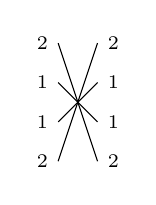
\begin{tikzpicture}[scale=.5,baseline=-20]
\node at (-.4,0) {$\scriptstyle 2$};
\node at (-.4,-1) {$\scriptstyle 1$};
\node at (-.4,-2) {$\scriptstyle{\ol1}$};
\node at (-.4,-3) {$\scriptstyle{\ol2}$};  
\node at (1.4,0) {$\scriptstyle 2$};
\node at (1.4,-1) {$\scriptstyle 1$};
\node at (1.4,-2) {$\scriptstyle{\ol1}$};
\node at (1.4,-3) {$\scriptstyle{\ol2}$};  
\draw[-] (0,0) -- (1,-3);
\draw[-] (0,-1) -- (1,-2);
\draw[-] (0,-2) -- (1,-1);
\draw[-] (0,-3) -- (1,0);
\end{tikzpicture}%,
,\\
\phantom{\sum}\ntksp F_{[\ol2,2]}\phantom{\sum}
\end{gathered}
\begin{gathered}
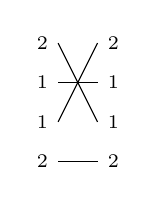
\begin{tikzpicture}[scale=.5,baseline=-20]
\node at (-.4,0) {$\scriptstyle 2$};
\node at (-.4,-1) {$\scriptstyle 1$};
\node at (-.4,-2) {$\scriptstyle{\ol1}$};
\node at (-.4,-3) {$\scriptstyle{\ol2}$};  
\node at (1.4,0) {$\scriptstyle 2$};
\node at (1.4,-1) {$\scriptstyle 1$};
\node at (1.4,-2) {$\scriptstyle{\ol1}$};
\node at (1.4,-3) {$\scriptstyle{\ol2}$};  
\draw[-] (0,0) -- (1,-2);
\draw[-] (0,-1) -- (1,-1);
\draw[-] (0,-2) -- (1,0);
\draw[-] (0,-3) -- (1,-3);
\end{tikzpicture},\\
   \phantom{\sum}\ntksp F_{[\ol1,2]}\phantom{\sum}
 \end{gathered}
\begin{gathered}
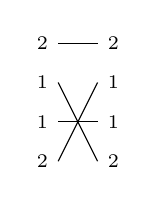
\begin{tikzpicture}[scale=.5,baseline=-20]
\node at (-.4,0) {$\scriptstyle 2$};
\node at (-.4,-1) {$\scriptstyle 1$};
\node at (-.4,-2) {$\scriptstyle{\ol1}$};
\node at (-.4,-3) {$\scriptstyle{\ol2}$};  
\node at (1.4,0) {$\scriptstyle 2$};
\node at (1.4,-1) {$\scriptstyle 1$};
\node at (1.4,-2) {$\scriptstyle{\ol1}$};
\node at (1.4,-3) {$\scriptstyle{\ol2}$};  
\draw[-] (0,0) -- (1,0);
\draw[-] (0,-1) -- (1,-3);
\draw[-] (0,-2) -- (1,-2);
\draw[-] (0,-3) -- (1,-1);
\end{tikzpicture},\\
   \phantom{\sum}\ntksp F_{[\ol2,1]}\phantom{\sum}
 \end{gathered}
\begin{gathered}
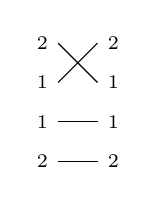
\begin{tikzpicture}[scale=.5,baseline=-20]
\node at (-.4,0) {$\scriptstyle 2$};
\node at (-.4,-1) {$\scriptstyle 1$};
\node at (-.4,-2) {$\scriptstyle{\ol1}$};
\node at (-.4,-3) {$\scriptstyle{\ol2}$};  
\node at (1.4,0) {$\scriptstyle 2$};
\node at (1.4,-1) {$\scriptstyle 1$};
\node at (1.4,-2) {$\scriptstyle{\ol1}$};
\node at (1.4,-3) {$\scriptstyle{\ol2}$};  
\draw[-] (0,0) -- (1,-1);
\draw[-] (0,-1) -- (1,0);
\draw[-] (0,-2) -- (1,-2);
\draw[-] (0,-3) -- (1,-3);
\end{tikzpicture},\\
   \phantom{\sum}\ntksp F_{[1,2]}\phantom{\sum}
 \end{gathered}
\begin{gathered}
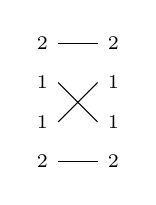
\begin{tikzpicture}[scale=.5,baseline=-20]
\node at (-.4,0) {$\scriptstyle 2$};
\node at (-.4,-1) {$\scriptstyle 1$};
\node at (-.4,-2) {$\scriptstyle{\ol1}$};
\node at (-.4,-3) {$\scriptstyle{\ol2}$};  
\node at (1.4,0) {$\scriptstyle 2$};
\node at (1.4,-1) {$\scriptstyle 1$};
\node at (1.4,-2) {$\scriptstyle{\ol1}$};
\node at (1.4,-3) {$\scriptstyle{\ol2}$};  
\draw[-] (0,0) -- (1,0);
\draw[-] (0,-1) -- (1,-2);
\draw[-] (0,-2) -- (1,-1);
\draw[-] (0,-3) -- (1,-3);
\end{tikzpicture},\\
   \phantom{\sum}\ntksp F_{[\ol1,1]}\phantom{\sum}
 \end{gathered}
\begin{gathered}
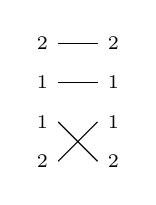
\begin{tikzpicture}[scale=.5,baseline=-20]
\node at (-.4,0) {$\scriptstyle 2$};
\node at (-.4,-1) {$\scriptstyle 1$};
\node at (-.4,-2) {$\scriptstyle{\ol1}$};
\node at (-.4,-3) {$\scriptstyle{\ol2}$};  
\node at (1.4,0) {$\scriptstyle 2$};
\node at (1.4,-1) {$\scriptstyle 1$};
\node at (1.4,-2) {$\scriptstyle{\ol1}$};
\node at (1.4,-3) {$\scriptstyle{\ol2}$};  
\draw[-] (0,0) -- (1,0);
\draw[-] (0,-1) -- (1,-1);
\draw[-] (0,-2) -- (1,-3);
\draw[-] (0,-3) -- (1,-2);
\end{tikzpicture},\\
   \phantom{\sum}\ntksp F_{[\ol2,\ol1]}\phantom{\sum}
 \end{gathered}
\
\begin{gathered}
\begin{tikzpicture}[scale=.5,baseline=-20]
\node at (-.4,0) {$\scriptstyle 2$};
\node at (-.4,-1) {$\scriptstyle 1$};
\node at (-.4,-2) {$\scriptstyle{\ol1}$};
\node at (-.4,-3) {$\scriptstyle{\ol2}$};  
\node at (1.4,0) {$\scriptstyle 2$};
\node at (1.4,-1) {$\scriptstyle 1$};
\node at (1.4,-2) {$\scriptstyle{\ol1}$};
\node at (1.4,-3) {$\scriptstyle{\ol2}$};  
\draw[-] (0,0) -- (1,0);
\draw[-] (0,-1) -- (1,-1);
\draw[-] (0,-2) -- (1,-2);
\draw[-] (0,-3) -- (1,-3);
\end{tikzpicture},\\
\phantom{\sum}\ntksp F_\emptyset \phantom{\sum}
 \end{gathered}
\end{equation}
where $F_\emptyset = F_{[\ol2,\ol2]} = F_{[\ol1,\ol1]} = F_{[1,1]} = F_{[2,2]}$.
In figures,
all edges in planar networks
should be understood to be oriented from left to right,
with vertices at both ends of all line
segments, and additional vertices at the centers of the
stars formed from crossing line segments.
Thus $F_{\smash{[\ol1,2]}}$ above can be more completely drawn as
\begin{equation*}
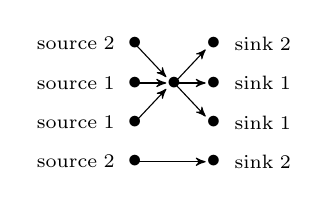
\begin{tikzpicture}[scale=.5,baseline=15]
\node at (-2.5,2.5) {$\scriptstyle{ \mathrm{source}\;2}$};
\node at (-2.5,1.5) {$\scriptstyle{ \mathrm{source}\;1}$};
\node at (-2.5,0.5) {$\scriptstyle{ \mathrm{source}\;\ol1}$};
\node at (-2.5,-0.5) {$\scriptstyle{ \mathrm{source}\;\ol2}$};  
\node at (2.25,2.5) {$\scriptstyle{ \mathrm{sink}\;2}$};
\node at (2.25,1.5) {$\scriptstyle{ \mathrm{sink}\;1}$};
\node at (2.25,0.5) {$\scriptstyle{ \mathrm{sink}\;\ol1}$};
\node at (2.25,-0.5) {$\scriptstyle{ \mathrm{sink}\;\ol2}$};  
\draw[->,>=stealth'] (-1,2.5) -- (-.2,1.65);
\draw[->,>=stealth'] (-1,1.5) -- (-.2,1.5);
\draw[->,>=stealth'] (-1,0.5) -- (-.2,1.35);
\draw[->,>=stealth'] (0,1.5) -- (.8,2.35);
\draw[->,>=stealth'] (0,1.5) -- (.8,1.5);
\draw[->,>=stealth'] (0,1.5) -- (.8,0.65);
\draw[->,>=stealth'] (-1,-0.5) -- (.8,-0.5);
\node at (-1,2.5) {$\bullet$}; 
\node at (-1,1.5) {$\bullet$}; 
\node at (-1,0.5) {$\bullet$}; 
\node at (-1,-0.5) {$\bullet$};
\node at (1,2.5) {$\bullet$}; 
\node at (1,1.5) {$\bullet$}; 
\node at (1,0.5) {$\bullet$}; 
\node at (1,-0.5) {$\bullet$};
\node at (0,1.5) {$\bullet$};
\end{tikzpicture}
\ .
\end{equation*}  
For economy, we will omit edge orientations and vertices from
drawings of planar networks.
When there is no danger of confusion, we will omit source and sink labels
as well. 


Given networks $E, F \in \net{A}{[h,l]}$,
in which all sources have
outdegree $1$ and all sinks have indegree $1$, define
the concatenation $E \circ F$ of $E$ and $F$
as follows.  For $i = h,\dotsc, l$, do
\begin{enumerate}
\item remove sink $i$ of $E$ and source $i$ of $F$,
\item merge each edge $(\vertex x, \text{sink }i)$ in $E$ with each edge
  $( \text{source }i, \vertex y )$ in $F$
  to form a single edge $(\vertex x, \vertex y)$ in $E \circ F$.
\end{enumerate}
Observe that for
nonintersecting intervals $[c_1,d_1]$, $[c_2,d_2]$,
the concatenations
$F_{[c_1,d_1]} \circ F_{[c_2,d_2]}$ and 
$F_{[c_2,d_2]} \circ F_{[c_1,d_1]}$ are
isomorphic as directed graphs.
Observe also that sometimes in a concatenation $E \circ F$,
there may exist vertices $\vertex x$ in $E$, $\vertex y$ in $F$
with
$m(\vertex x, \vertex y) > 1$ multiplicity-$1$ edges
incident upon both.
Define the {\em condensed concatenation}
$E \bullet F$ to be the
subdigraph of $E \circ F$ obtained
by removing, for all such pairs $(\vertex x, \vertex y)$,
all but one of the $m(\vertex x, \vertex y)$ edges incident upon both,
and by marking this edge with the multiplicity $m(\vertex x, \vertex y)$.
For example, in $\net A{[\ol2,2]}$ we have the isomorphic graphs
\begin{equation}\label{eq:allbutone1}
F_{[\ol2,\ol1]} \circ F_{[1,2]} =
F_{[\ol2,\ol1]} \bullet F_{[1,2]} =
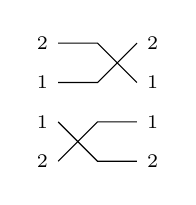
\begin{tikzpicture}[scale=.5,baseline=0]
\node at (-.4,1.5) {$\scriptstyle 2$};
\node at (-.4,0.5) {$\scriptstyle 1$};
\node at (-.4,-0.5) {$\scriptstyle{\ol1}$};
\node at (-.4,-1.5) {$\scriptstyle{\ol2}$};  
\node at (2.4,1.5) {$\scriptstyle 2$};
\node at (2.4,0.5) {$\scriptstyle 1$};
\node at (2.4,-0.5) {$\scriptstyle{\ol1}$};
\node at (2.4,-1.5) {$\scriptstyle{\ol2}$};  
\draw[-] (0,1.5) -- (1,1.5) -- (2,0.5);
\draw[-] (0,0.5) -- (1,0.5) -- (2,1.5);
\draw[-] (0,-0.5) -- (1,-1.5) -- (2,-1.5);
\draw[-] (0,-1.5) -- (1,-0.5) -- (2,-0.5);
\end{tikzpicture}
\cong
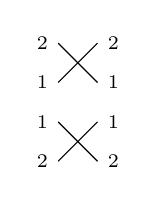
\begin{tikzpicture}[scale=.5,baseline=0]
\node at (-.4,1.5) {$\scriptstyle 2$};
\node at (-.4,0.5) {$\scriptstyle 1$};
\node at (-.4,-0.5) {$\scriptstyle{\ol1}$};
\node at (-.4,-1.5) {$\scriptstyle{\ol2}$};  
\node at (1.4,1.5) {$\scriptstyle 2$};
\node at (1.4,0.5) {$\scriptstyle 1$};
\node at (1.4,-0.5) {$\scriptstyle{\ol1}$};
\node at (1.4,-1.5) {$\scriptstyle{\ol2}$};  
\draw[-] (0,1.5) -- (1,0.5);% -- (2,0.5);
\draw[-] (0,0.5) -- (1,1.5);% -- (2,1.5);
\draw[-] (0,-0.5) -- (1,-1.5);% -- (2,-1.5);
\draw[-] (0,-1.5) -- (1,-0.5);% -- (2,-0.5);
\end{tikzpicture}
\;\cong\;
F_{[1,2]} \circ F_{[\ol2,\ol1]} =
F_{[1,2]} \bullet F_{[\ol2,\ol1]},
\end{equation}
and the nonisomorphic graphs
\begin{equation}\label{eq:allbutone2}
  F_{[\ol2,1]} \circ F_{[\ol1,2]} \circ F_{[\ol2,1]} =
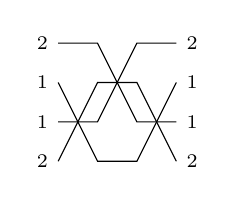
\begin{tikzpicture}[scale=.5,baseline=0]
\node at (-.4,1.5) {$\scriptstyle 2$};
\node at (-.4,0.5) {$\scriptstyle 1$};
\node at (-.4,-0.5) {$\scriptstyle{\ol1}$};
\node at (-.4,-1.5) {$\scriptstyle{\ol2}$};  
\node at (3.4,1.5) {$\scriptstyle 2$};
\node at (3.4,0.5) {$\scriptstyle 1$};
\node at (3.4,-0.5) {$\scriptstyle{\ol1}$};
\node at (3.4,-1.5) {$\scriptstyle{\ol2}$};  
\draw[-] (0,1.5) -- (1,1.5) -- (2,-0.5) -- (3,-0.5);
\draw[-] (0,0.5) -- (1,-1.5) -- (2,-1.5) -- (3,0.5);
\draw[-] (0,-0.5) -- (1,-0.5) -- (2,1.5) -- (3,1.5);
\draw[-] (0,-1.5) -- (1,0.5) -- (2,0.5) -- (3,-1.5);
\end{tikzpicture}
\; \not \cong \;
  F_{[\ol2,1]} \bullet F_{[\ol1,2]} \bullet F_{[\ol2,1]} =
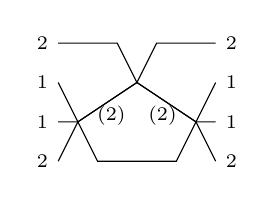
\begin{tikzpicture}[scale=.5,baseline=0]
\node at (-0.9,1.5) {$\scriptstyle 2$};
\node at (-0.9,0.5) {$\scriptstyle 1$};
\node at (-0.9,-0.5) {$\scriptstyle{\ol1}$};
\node at (-0.9,-1.5) {$\scriptstyle{\ol2}$};  
\node at (2.15,-.35) {$\scriptstyle (2)$};
\node at (.85,-.35) {$\scriptstyle (2)$};
\node at (3.9,1.5) {$\scriptstyle 2$};
\node at (3.9,0.5) {$\scriptstyle 1$};
\node at (3.9,-0.5) {$\scriptstyle{\ol1}$};
\node at (3.9,-1.5) {$\scriptstyle{\ol2}$};  
\draw[-] (-0.5,1.5) -- (1,1.5) -- (1.5,0.5) -- (2,1.5) -- (3.5,1.5);
\draw[-] (-0.5,0.5) -- (-0,-0.5) -- (1.5,0.5) -- (3,-0.5) -- (3.5,0.5);
\draw[-] (-0.5,-0.5) -- (-0,-0.5) -- (1.5,0.5) -- (3,-0.5) -- (3.5,-0.5);
\draw[-] (-0.5,-1.5) -- (-0,-0.5) -- (.5,-1.5) -- (2.5,-1.5) -- (3,-0.5) -- (3.5,-1.5);
\end{tikzpicture},
\end{equation}
in which two pairs of edges are replaced by two single edges
marked with multiplicity $2$.
We refer to all iterations of concatenations and condensed concatenations
of simple star networks as {\em star networks}.
In fact, each element of $\net A{[h,l]}$ is isomorphic to a star network,
so we may think of $\net A{[h,l]}$ as a set of
star networks.


Given planar network $F \in \net A{[h,l]}$, define
its {\em path matrix} $A = A(F) = (a_{i,j})_{i,j \in [h,l]}$ by
\begin{equation}\label{eq:pathmatrix}
  a_{i,j} = \# \text{ paths in $F$ from source $i$ to sink $j$},
\end{equation}
ignoring multiplicities.
For instance, the star networks in
\eqref{eq:allbutone1} -- \eqref{eq:allbutone2}
have path matrices
\begin{equation*}
  \begin{bmatrix}
    a_{\ol2,\ol2} & a_{\ol2, \ol1} & a_{\ol2, 1} & a_{\ol2, 2} \\
    a_{\ol1,\ol2} & a_{\ol1, \ol1} & a_{\ol1, 1} & a_{\ol1, 2} \\
    a_{1,\ol2}   & a_{1, \ol1}   & a_{1, 1}   & a_{1, 2} \\
    a_{2,\ol2}   & a_{2, \ol1}   & a_{2, 1}   & a_{2, 2} 
  \end{bmatrix}
  \quad
  = 
  \quad
  \begin{bmatrix}
    1 & 1 & 0 & 0 \\
    1 & 1 & 0 & 0 \\
    0 & 0 & 1 & 1 \\
    0 & 0 & 1 & 1     
  \end{bmatrix}\ntksp,
  \
  \begin{bmatrix}
    5 & 5 & 5 & 2 \\
    5 & 5 & 5 & 2 \\
    5 & 5 & 5 & 2 \\
    2 & 2 & 2 & 1
  \end{bmatrix}\ntksp,
  \
  \begin{bmatrix}
    2 & 2 & 2 & 1 \\
    2 & 2 & 2 & 1 \\
    2 & 2 & 2 & 1 \\
    1 & 1 & 1 & 1     
  \end{bmatrix}\ntksp,
\end{equation*}
respectively.

\begin{defn}\label{d:starnet}
Define $\snet{A}{[h,l]}$ to be set of all type-$\msfA$ planar networks of the
form
\begin{equation}\label{eq:bulletconcat}
    F = F_{[c_1,d_1]} \bullet \cdots \bullet F_{[c_t,d_t]}, \\
\end{equation}
and call these
{\em type-$\msfA$ condensed star networks
  (with boundary vertices indexed by $[h,l]$)}.
\end{defn}

We will be interested in two subclasses of these,
which we define as follows.
\begin{defn}\label{d:zz}
  Call a type-$\msfA$ condensed star network $F$
  \eqref{eq:bulletconcat}  
  a {\em type-$\msfA$ zig-zag network}
  if we have $F=F_\emptyset$ or 
  \begin{enumerate}
\item the intervals $[c_1,d_1], \dotsc, [c_t,d_t]$
  are distinct and pairwise nonnesting,
\item for all triples
  $i < j < k$ satisfying
  $[c_i,d_i] \cap [c_j,d_j] \neq \emptyset$ and 
$[c_j,d_j] \cap [c_k,d_k] \neq \emptyset$,
  we have
$c_i < c_j < c_k$ 
(and $d_i < d_j < d_k$) 
or $c_i > c_j > c_k$
(and $d_i > d_j > d_k$).
  \end{enumerate}
\end{defn}
Let $\znet{A}{[h,l]}$ denote the set of type-$\msfA$ zig-zag networks
  with boundary vertices indexed by $[h,l]$.
\begin{defn}\label{d:adsn}
  Call a type-$\msfA$ condensed star network $F$ \eqref{eq:bulletconcat}  
  a {\em type-$\msfA$ descending star network}
  if we have $F=F_\emptyset$ or 
  \begin{enumerate}
\item the intervals $[c_1,d_1], \dotsc, [c_t,d_t]$
  are distinct and pairwise nonnesting,
\item for all pairs
  $i < j$ satisfying
  $[c_i,d_i] \cap [c_j,d_j] \neq \emptyset$
  we have $c_i > c_j$ (and $d_i > d_j$).
  \end{enumerate}
\end{defn}
Let $\dnet{A}{[h,l]}$ denote the set of type-$\msfA$ descending star networks
with boundary vertices indexed by $[h,l]$.
Thus we have $\dnet{A}{[h,l]} \subseteq \znet{A}{[h,l]}$.
To illustrate, let us fix boundary vertices
indexed by any interval of cardinality $4$.
Then we have $14$ descending star networks,
\begin{equation}\label{eq:xfigures2}
\raisebox{-.5\height}{
\begin{tikzpicture}
\node at (0, 0) {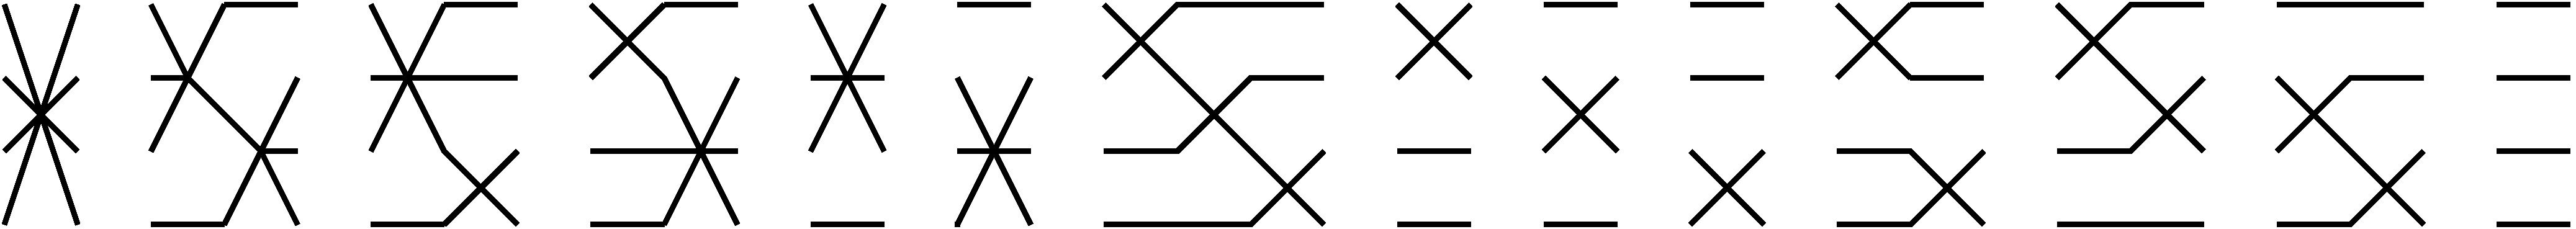
\includegraphics[height=10.2mm]{../assets/775/xfigures2.pdf}};
\node at (-4.63, 0.15) {$\scriptscriptstyle{(2)}$};
\end{tikzpicture}
}
\end{equation}
and $8$ more zig-zag networks
which are not descending star networks,
\begin{equation}\label{eq:xfigureszz}
\raisebox{-.5\height}{
\begin{tikzpicture}
\node at (0, 0) {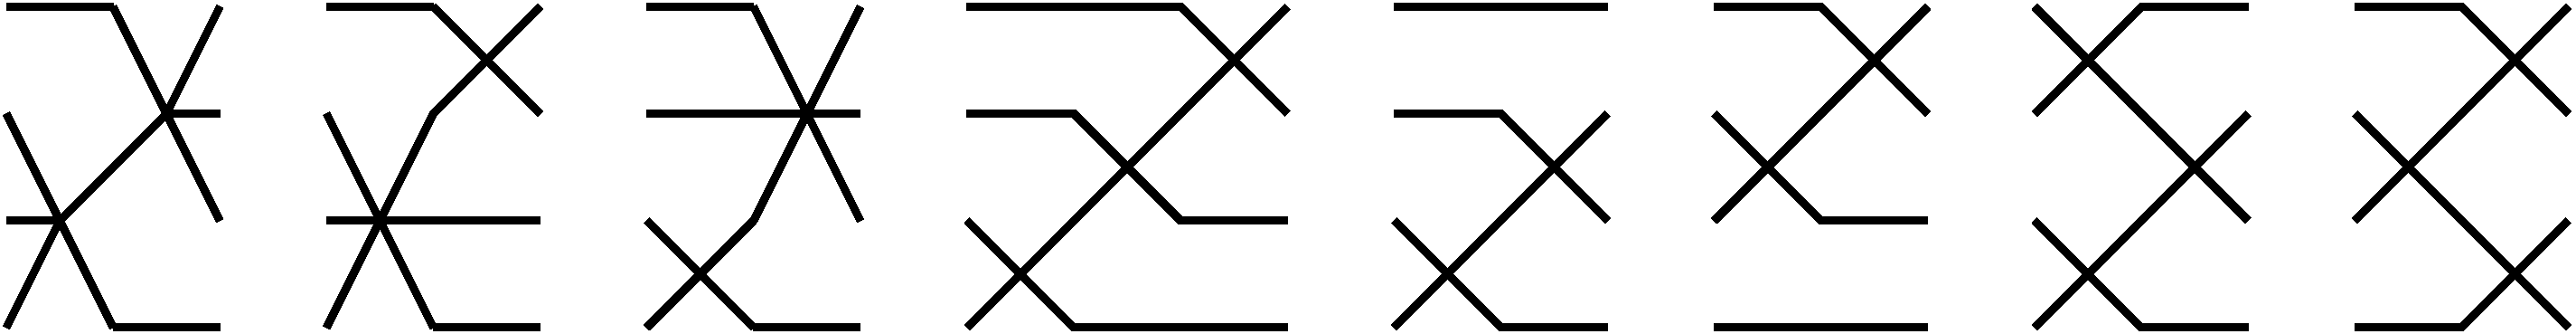
\includegraphics[height=10.2mm]{../assets/775/xfigureszz.pdf}};
\node at (-3.68, 0.15) {$\scriptscriptstyle{(2)}$};
\node at (4.1, 0) {.};
\end{tikzpicture}
}
\end{equation}

The result \cite[Lem.\,3.5]{CHSSkanEKL}
describes intersections of paths in a descending star network.
\begin{lem}\label{l:lemma3.5}
  Let $\pi_{i_1}$, $\pi_{i_2}$ be paths in a descending star network $F$
  from sources $i_1 < i_2$ to sinks $m_1$, $m_2$, respectively.
  Then the two paths intersect if and only if there exists a path in $F$
  from $i_1$ to sink $m_2$.
  \end{lem}

By \cite[Thm.\,3.5, Lem.\,5.3]{SkanNNDCB}
and \cite[Thm.\,3.6]{CHSSkanEKL},
the sets
$\dnet{A}{[h,l]}$, $\znet{A}{[h,l]}$
are related to pattern avoidance in $\mfs{[h,l]}$.
\begin{prop}\label{p:anetpavoid}
There is a natural bijection $F \mapsto w(F)$ from 
$\znet{A}{[h,l]}$
to \pavoiding permutations in $\mfs{[h,l]}$,
which restricts to a bijection from $\dnet{A}{[h,l]}$ to
$312$-avoiding permutations in $\mfs{[h,l]}$.
\end{prop}
To describe
the bijection
explicitly
we
define
a relation $\precdot$
on the set of intervals appearing in \eqref{eq:bulletconcat}
by
declaring
\begin{equation}\label{eq:precdotdef}
  [c_i,d_i] \precdot [c_j,d_j]
  \end{equation}
if 
$i < j$ and
$[c_i,d_i] \cap [c_j,d_j] \ssm ( [c_{i+1},d_{i+1}] \cup \cdots \cup [c_{j-1},d_{j-1}]) \neq \emptyset$.
  The relation $\precdot$ may be viewed as an acyclic directed graph on 
  the intervals.
  The transitive, reflexive closure of $\precdot$ is a partial order $\preceq$.
  For $F \in \znet{A}{[h,l]}$, the directed graph is the Hasse diagram
  of the partial order; for other $F \in \snet A{[h,l]}$ this is not the case.
  For example, the networks
  $F_{[2,5]} \bullet F_{[1,3]} \bullet F_{[4,6]} \bullet F_{[6,7]}
  \in \znet A{[1,7]}$
  and
  $F_{[2,5]} \bullet F_{[1,2]} \bullet F_{[4,6]} \bullet F_{[2,5]}
  \in \snet{A}{[1,7]}$
and their corresponding interval digraphs and posets are
\begin{equation}\label{eq:posetex}
  \begin{gathered}
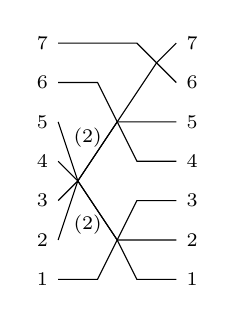
\begin{tikzpicture}[scale=.5,baseline=55]
  \node at (-.4,7) {$\scriptstyle 7$};
  \node at (-.4,6) {$\scriptstyle 6$};
  \node at (-.4,5) {$\scriptstyle 5$};
  \node at (-.4,4) {$\scriptstyle 4$};
  \node at (-.4,3) {$\scriptstyle 3$};
  \node at (-.4,2) {$\scriptstyle 2$};
  \node at (-.4,1) {$\scriptstyle 1$};
  \node at (3.4,7) {$\scriptstyle 7$};
  \node at (3.4,6) {$\scriptstyle 6$};
  \node at (3.4,5) {$\scriptstyle 5$};
  \node at (3.4,4) {$\scriptstyle 4$};
  \node at (3.4,3) {$\scriptstyle 3$};
  \node at (3.4,2) {$\scriptstyle 2$};
  \node at (3.4,1) {$\scriptstyle 1$};
\draw[-] (0,7) -- (2,7) -- (3,6);
\draw[-] (0,6) -- (1,6) -- (2,4) -- (3,4);
\draw[-] (0,5) -- (0.5,3.5) -- (1.5,2) -- (2,1) -- (3,1);
\draw[-] (0,4) -- (0.5,3.5) -- (1.5,2) -- (3,2);
\draw[-] (0,3) -- (0.5,3.5) -- (1.5,5) -- (3,5);
\draw[-] (0,2) -- (0.5,3.5) -- (1.5,5) -- (2.5,6.5) -- (3,7);
\draw[-] (0,1) -- (1,1) -- (2,3) -- (3,3);
\node at (0.75,4.6) {$\scriptstyle{(2)}$};
\node at (0.75,2.4) {$\scriptstyle{(2)}$};
\end{tikzpicture},
  \qquad \qquad
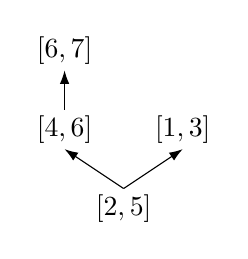
\begin{tikzpicture}[scale=.5,baseline=15]
\node at (0,1) {$[1, 3]$};            %\node at (1,5.5) {$n$};
\node at (-1.5,-1) {$[2,5]$};          %\node at (1.75,4.5) {$n-1$};
\node at (-3,1) {$[4,6]$};            %\node at (1,1.5) {$2$};
\node at (-3,3) {$[6,7]$};            %\node at (1,5.5) {$n$};
\draw[->] (-3,1.5) -- (-3,2.5);
\draw[<-] (0,0.5) -- (-1.5,-0.5);
\draw[<-] (-3,0.5) -- (-1.5,-0.5);
\end{tikzpicture},
  \qquad \qquad
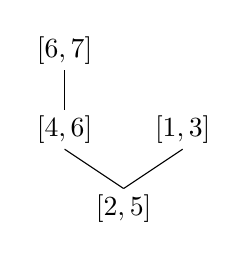
\begin{tikzpicture}[scale=.5,baseline=15]
\node at (0,1) {$[1, 3]$};            %\node at (1,5.5) {$n$};
\node at (-1.5,-1) {$[2,5]$};          %\node at (1.75,4.5) {$n-1$};
\node at (-3,1) {$[4,6]$};            %\node at (1,1.5) {$2$};
\node at (-3,3) {$[6,7]$};            %\node at (1,5.5) {$n$};
\draw[-] (-3,1.5) -- (-3,2.5);
\draw[-] (0,0.5) -- (-1.5,-0.5);
\draw[-] (-3,0.5) -- (-1.5,-0.5);
\end{tikzpicture}\qquad\qquad \\
\qquad\qquad
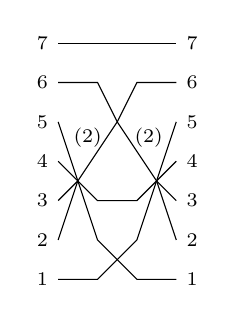
\begin{tikzpicture}[scale=.5,baseline=55]
  \node at (-.4,7) {$\scriptstyle 7$};
  \node at (-.4,6) {$\scriptstyle 6$};
  \node at (-.4,5) {$\scriptstyle 5$};
  \node at (-.4,4) {$\scriptstyle 4$};
  \node at (-.4,3) {$\scriptstyle 3$};
  \node at (-.4,2) {$\scriptstyle 2$};
  \node at (-.4,1) {$\scriptstyle 1$};
  \node at (3.4,7) {$\scriptstyle 7$};
  \node at (3.4,6) {$\scriptstyle 6$};
  \node at (3.4,5) {$\scriptstyle 5$};
  \node at (3.4,4) {$\scriptstyle 4$};
  \node at (3.4,3) {$\scriptstyle 3$};
  \node at (3.4,2) {$\scriptstyle 2$};
  \node at (3.4,1) {$\scriptstyle 1$};
\draw[-] (0,7) -- (3,7);
\draw[-] (0,6) -- (1,6) -- (1.5,5) -- (2.5,3.5) -- (3,2);
\draw[-] (0,5) -- (1,2) -- (2,1) -- (3,1);
\draw[-] (0,4) -- (1,3) -- (2,3) -- (3,4);
\draw[-] (0,3) -- (0.5,3.5) -- (1.5,5) -- (2,6) -- (3,6);
\draw[-] (0,2) -- (0.5,3.5);
\draw[-] (2.5,3.5) -- (3,3);
\draw[-] (0,1) -- (1,1) -- (2,2) -- (3,5);
\node at (0.75,4.6) {$\scriptstyle{(2)}$};
\node at (2.3,4.6) {$\scriptstyle{(2)}$};
\end{tikzpicture},
  \qquad \qquad
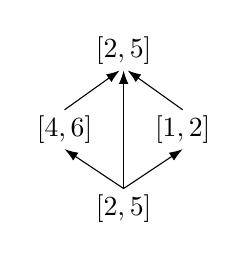
\begin{tikzpicture}[scale=.5,baseline=15]
\node at (0,1) {$[1, 2]$};            %\node at (1,5.5) {$n$};
\node at (-1.5,-1) {$[2,5]$};         %\node at (1.75,4.5) {$n-1$};
\node at (-3,1) {$[4,6]$};            %\node at (1,1.5) {$2$};
\node at (-1.5,3) {$[2,5]$};            %\node at (1,5.5) {$n$};
\draw[->] (-3,1.5) -- (-1.6,2.5);
\draw[->] (0,1.5) -- (-1.4,2.5);
\draw[->] (-1.5,-0.5) -- (-1.5,2.5);
\draw[<-] (0,0.5) -- (-1.5,-0.5);
\draw[<-] (-3,0.5) -- (-1.5,-0.5);
\end{tikzpicture},
  \qquad \qquad
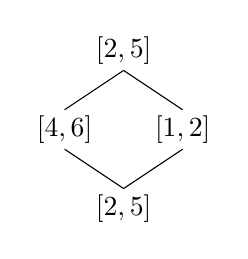
\begin{tikzpicture}[scale=.5,baseline=15]
\node at (0,1) {$[1,2]$};            %\node at (1,5.5) {$n$};
\node at (-1.5,-1) {$[2,5]$};          %\node at (1.75,4.5) {$n-1$};
\node at (-3,1) {$[4,6]$};            %\node at (1,1.5) {$2$};
\node at (-1.5,3) {$[2,5]$};            %\node at (1,5.5) {$n$};
\draw[-] (-3,1.5) -- (-1.5,2.5);
\draw[-] (0,1.5) -- (-1.5,2.5);
\draw[-] (0,0.5) -- (-1.5,-0.5);
\draw[-] (-3,0.5) -- (-1.5,-0.5);
\end{tikzpicture}.
\end{gathered}
\end{equation}
The bijection $F \mapsto w(F)$,
stated in
\cite[\S 3]{SkanNNDCB},
is given by the following algorithm.
\begin{alg}\label{a:FwF}
  Given $F$ as in \eqref{eq:bulletconcat}, do
  \begin{enumerate}
\item 
  Initialize the sequence of reversals
  $S \defeq (s_{[c_1,d_1]}, \dotsc, s_{[c_t,d_t]})$.
\item 
  For all pairs $(i,j)$ with $[c_i,d_i] \precdot [c_j,d_j]$ and
  $|[c_i,d_i] \cap [c_j,d_j]| > 1$,
 \begin{enumerate}[]
 \item Update $S$ by inserting $s_{[c_i,d_i] \cap [c_j,d_j]}$
   immediately after $s_{[c_i,d_i]}$.
 \end{enumerate}
\item Define $w(F)$ to be the product of reversals in $S$, from left to right.
\end{enumerate}
\end{alg}
We call the final sequence of reversals a
{\em zig-zag factorization} of $w(F)$.
For example, let $F$ be the first star network in \eqref{eq:posetex}.
This zig-zag network $F$ gives the
reversal sequence $(s_{[2,5]}, s_{[1,3]}, s_{[4,6]}, s_{[6,7]})$ which we update
by inserting $s_{[2,5] \cap [1,3]} = s_{[2,3]}$ after $s_{[2,5]}$, and then
$s_{[2,5] \cap [4,6]} = s_{[4,5]}$ after $s_{[2,5]}$ to obtain
the permutation
\begin{equation*}
  w = w(F) = s_{[2,5]}s_{[4,5]}s_{[2,3]}s_{[1,3]}s_{[4,6]}s_{[6,7]} = 3752146.
  \end{equation*}

The inverse of the map $F \mapsto w(F)$,
which we write
\begin{equation}\label{eq:wFw}
  w \mapsto F_w,
\end{equation}
is a bit intricate and is given in~\cite[\S 3]{SkanNNDCB}.
It turns out that the network $F$ above is $F_{3752146}$.
In \eqref{eq:xfigures2}, if we label sources and sinks $1, 2, 3, 4$ from bottom
to top, the descending star networks are
\begin{equation}\label{eq:dsnlist}
  \begin{gathered}
  F_{4321}, F_{3421}, F_{2431}, F_{3241}, F_{1432}, F_{3214}, F_{2341}, F_{1243}, F_{1324}, F_{2134}, \\
  F_{2143}, F_{1342}, F_{2314}, F_{1234},
  \end{gathered}
\end{equation}
respectively.
In \eqref{eq:xfigureszz}, the remaining zig-zag networks are
\begin{equation}\label{eq:zzlist}
  F_{4312}, F_{4213}, F_{4132}, F_{4123}, F_{3124}, F_{1423}, F_{1423}, F_{3142}, F_{2413}.
  \end{equation}
The restriction of the map \eqref{eq:wFw} to $312$-avoiding elements of $\sn$
is in fact rather simple.  Given word $w = w_1 \cdots w_n$
with distinct letters,
say that $w$ has a {\em record} at position $j$
if $w_j = \max\{ w_1, \dotsc, w_j \}$.

\begin{alg}\label{a:wFw}
  Given $w = w_1 \cdots w_n \in \sn$ avoiding the pattern $312$, do
  \begin{enumerate}
  \item Let $w$ have records at positions $1 = j_1, \dotsc, j_k$.
  \item Define
    $F_w = F_{[j_k,w_{j_k}]}
    \bullet \cdots \bullet F_{[j_1,w_{j_1}]}$.
  \end{enumerate}
\end{alg}

The bijection $F \mapsto w(F)$ is closely related to
families of source-to-sink paths in $F$, and also to Kazhdan--Lusztig
basis elements of the Hecke algebra of $\mfs{[h,l]}$. 
Given $F \in \net A{[h,l]}$,
call a sequence $\pi = (\pi_h,\dotsc,\pi_l)$ of paths in $F$
a {\em path family of type $w = w_h \cdots w_l$} if for $i = h,\dotsc,l$,
path $\pi_i$ begins at source $i$ and ends at sink $w_i$.
Say that a path family $\pi$ {\em covers} $F$ if every edge of $F$
appears in at least one path of $\pi$, and define the sets
\begin{equation}
  \begin{gathered}
    \Pi(F) = \{ \pi \,|\, \pi \text{ covers } F \},\\
    \Pi_w(F) = \{ \pi \in \Pi(F) \,|\, \type(\pi) = w \}.
  \end{gathered}
\end{equation}
For example,
the star network
and path family
\begin{equation}\label{eq:132313}
F = F_{[1,3]} \circ F_{[2,3]} \circ F_{[1,3]} = 
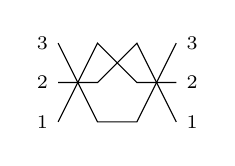
\begin{tikzpicture}[scale=.5,baseline=-10]
\node at (-.4,0.5) {$\scriptstyle 3$};
\node at (-.4,-0.5) {$\scriptstyle{2}$};
\node at (-.4,-1.5) {$\scriptstyle{1}$};  
\node at (3.4,0.5) {$\scriptstyle 3$};
\node at (3.4,-0.5) {$\scriptstyle{2}$};
\node at (3.4,-1.5) {$\scriptstyle{1}$};  
\draw[-] (0,0.5) -- (1,-1.5) -- (2,-1.5) -- (3,0.5);
\draw[-] (0,-0.5) -- (1,-0.5) -- (2,0.5) -- (3,-1.5);
\draw[-] (0,-1.5) -- (1,0.5) -- (2,-0.5) -- (3,-0.5);
\end{tikzpicture},\qquad
\pi = 
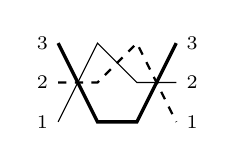
\begin{tikzpicture}[scale=.5,baseline=-10]
\node at (-.4,0.5) {$\scriptstyle 3$};
\node at (-.4,-0.5) {$\scriptstyle{2}$};
\node at (-.4,-1.5) {$\scriptstyle{1}$};  
\node at (3.4,0.5) {$\scriptstyle 3$};
\node at (3.4,-0.5) {$\scriptstyle{2}$};
\node at (3.4,-1.5) {$\scriptstyle{1}$};  
\draw[-, very thick] (0,0.5) -- (1,-1.5) -- (2,-1.5) -- (3,0.5);
\draw[-, thick, dashed] (0,-0.5) -- (1,-0.5) -- (2,0.5) -- (3,-1.5);
\draw[-] (0,-1.5) -- (1,0.5) -- (2,-0.5) -- (3,-0.5);
\end{tikzpicture}
\end{equation}
belong to $\net A{[1,3]}$ and $\Pi_{s_1}(F) \subset \Pi(F)$, respectively.
When $F$ is a zig-zag network,
we may characterize $w(F)$ in terms of $\Pi(F)$ as
follows~\cite[Lem.\,5.3]{SkanNNDCB}.
\begin{prop}\label{p:wFchar}  
  For $F \in \znet{A}{[h,l]}$,
$w(F)$ is the unique permutation of maximum length in
$\{ \type(\pi) \,|\, \pi \in \Pi(F) \} \subseteq \mfs{[h,l]}$.
\end{prop}


For all $F \in \net A{[h,l]}$, the set $\Pi(F)$ associates an element of
$\mathbb Z[\mfs{[h,l]}]$ to $F$:
we say that $F$ {\em graphically represents}
\begin{equation}\label{eq:Gtozsn}
\sum_{\pi \in \Pi(F)} \type(\pi)
\end{equation}
{\em as an element of $\mathbb Z[\mfs{[h,l]}]$}.
For example, the network $F$ in \eqref{eq:132313} can be covered by
$72$ different path families: $12$ of each type $w \in \mfs 3$.
Thus it graphically represents
$12\,\wtc{s_1s_2s_1}1$
as an element of $\mathbb Z [\mfs 3]$.

Again for all $F \in \net A{[h,l]}$,
the set $\Pi(F)$ also associates an element of
$H_{[h,l]}(q)$ to $F$.
To describe this element explicitly, we first assume
that $F$ is formed by some iteration of ordinary or condensed concatenation
of simple star networks $F_{[c_1,d_1]}, \dotsc, F_{[c_t,d_t]}$ with
internal vertices $\vertex z_1, \dotsc, \vertex z_t$. Observe that
the intersection of two source-to-sink paths $\pi_i$, $\pi_j$ in $F$
must be a disjoint union of the above internal vertices of $F$
and paths between these.
We say that $\pi_i$ and $\pi_j$ {\em meet} at a central vertex $\vertex z_k$
if both paths contain $\vertex z_k$, and enter it via different edges.
Given a path family $\pi$ covering $F$,
define a {\em defect} of $\pi$ to be a triple $(\pi_i, \pi_j, k)$ with
\begin{enumerate}
  \item $i < j$,
  \item $\pi_i$ and $\pi_j$ meet at vertex $\vertex z_k$ of
    $F$ after having crossed an odd number of times.
\end{enumerate}
Let $\dfct(\pi)$ denote the number of defects of $\pi$.
(This definition from \cite{CSkanTNNChar}
generalizes those of \cite{BWHex, Deodhar90}.)
We say that $F$ {\em graphically represents}
\begin{equation}\label{eq:Gtozhnq}
\sum_{\pi \in \Pi(F)} q^{\dfct(\pi)} T_{\type(\pi)}
\end{equation}
{\em as an element of $H_{[h,l]}(q)$}.
For example,
the path family $\pi$ in \eqref{eq:132313}
satisfies $\dfct(\pi) = 3$: the defects are
$(\pi_1, \pi_2, 2)$, $(\pi_1, \pi_3, 3)$, $(\pi_2, \pi_3, 3)$.
It is possible to show that the network $F$ in \eqref{eq:132313}
graphically represents
$(1+q)^2(1+q+q^2) \wtc{s_1s_2s_1}q$
as an element of $H_3(q)$.

It is clear that if $F$ graphically represents
$D(q) \in H_{[h,l]}(q)$ as an element of $H_{[h,l]}(q)$, then
it graphically represents
$D(1)$ as an element of $\mathbb Z[\mfs{[h,l]}]$.
It is possible to show that
all star networks
graphically represent products of Kazhdan--Lusztig basis elements
(possibly divided by integers or polynomials in $q$).
In particular, the result~\cite[Thm.\,1]{BWHex}
shows that sometimes such a product consists of a single 
Kazhdan--Lusztig basis element, and that the star network is a
{\em wiring diagram}, i.e. all intervals $[c_i,d_i]$ satisfy $d_i = c_i + 1$.
\begin{prop}
  Let
  $s_{c_1} \cdots s_{c_t}$ be a reduced expression for
  $w \in \mfs{[h,l]}$
  avoiding the patterns
  $321$, $56781234$, $56718234$, $46781235$, $46718235$.
  Then the star network
  $F_{[c_1,c_1+1]} \bullet \cdots \bullet F_{[c_t, c_t+1]}$
  graphically represents $\smash{\wtc wq}$
  as an element of
  $H_{[h,l]}(q)$.
\end{prop}
The result \cite[Lem.\,5.3]{SkanNNDCB} shows that zig-zag networks
give graphical representations of other Kazhdan--Lusztig basis elements.
\begin{prop}\label{p:pavoidrep}
  For $w \in \mfs{[h,l]}$ \avoidingp,
  the zig-zag network $F_w$ graphically represents $\wtc wq$
  as an element of $H_{[h,l]}(q)$.
\end{prop}

This fact has the following consequence.
\begin{cor}\label{c:atmostonepath}
      For $v, w \in \mfs{[h,l]}$ with $w$ \avoidingp,
      the number of path families of type $v$ covering $F_w$ is
      $1$ if $v \leq_{\mfs{[h,l]}} w$, and is $0$ otherwise.
\end{cor}


\ssec{Type-\texorpdfstring{$\msfBC$}{BC} planar networks and factorization}\label{ss:BCplanar}


For fixed $n$, define {\em type-$\msfBC$ simple star networks
  with boundary vertices indexed by $[\ol n, n]$} to be the
type-$\msfA$ star networks
\begin{equation}\label{eq:bcstardef}
  \begin{alignedat}{2}
    F'_{[a,b]} &\defeq F_{[a,b]} \bullet F_{[\ol a, \ol b]}
    = F_{[a,b]} \circ F_{[\ol a, \ol b]},
    &\qquad &1 \leq a \leq b \leq n, \\ 
    F'_{[\ol a, a]} &\defeq F_{[\ol a, a]},
    &\qquad &1 \leq a \leq n,
    \end{alignedat}
\end{equation}
which correspond naturally to the type-$\msfBC$ reversals \eqref{eq:creversal}.
For example the seven type-$\msfBC$
simple star networks
$F'_{\emptyset} = F'_{[1,1]} = F'_{[2,2]} = F'_{[3,3]}$ and $F'_{[1,2]}$,
$F'_{[2,3]}$, $F'_{[1,3]}$, $F'_{\smash{[\ol 1, 1]}}$, $F'_{\smash{[\ol 2, 2]}}$,
$F'_{\smash{[\ol 3, 3]}}$,
\begin{equation}\label{eq:csimplestars}        
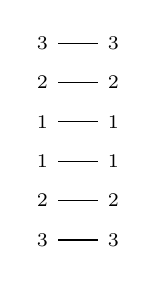
\begin{tikzpicture}[scale=.5,baseline=0]
  \node at (-.9,2.5) {$\scriptstyle 3$};
  \node at (-.9,1.5) {$\scriptstyle 2$};
  \node at (-.9,0.5) {$\scriptstyle 1$};
  \node at (0.9,2.5) {$\scriptstyle 3$};
  \node at (0.9,1.5) {$\scriptstyle 2$};
  \node at (0.9,0.5) {$\scriptstyle 1$};
  \node at (-.9,-2.5) {$\scriptstyle {\ol 3}$};
  \node at (-.9,-1.5) {$\scriptstyle {\ol 2}$};
  \node at (-.9,-0.5) {$\scriptstyle {\ol 1}$};
  \node at (0.9,-2.5) {$\scriptstyle {\ol 3}$};
  \node at (0.9,-1.5) {$\scriptstyle {\ol 2}$};
  \node at (0.9,-0.5) {$\scriptstyle {\ol 1}$};
\draw[-] (-.5,2.5) -- (.5,2.5);
\draw[-] (-.5,1.5) -- (.5,1.5);
\draw[-] (-.5,0.5) -- (.5,0.5);
\draw[-] (-.5,-0.5) -- (.5,-0.5);
\draw[-] (-.5,-1.5) -- (.5,-1.5);
\draw[-] (-.5,-2.5) -- (.5,-2.5);
\end{tikzpicture}
\ntnsp,\quad
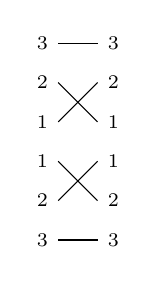
\begin{tikzpicture}[scale=.5,baseline=0]
  \node at (-.9,2.5) {$\scriptstyle 3$};
  \node at (-.9,1.5) {$\scriptstyle 2$};
  \node at (-.9,0.5) {$\scriptstyle 1$};
  \node at (0.9,2.5) {$\scriptstyle 3$};
  \node at (0.9,1.5) {$\scriptstyle 2$};
  \node at (0.9,0.5) {$\scriptstyle 1$};
  \node at (-.9,-2.5) {$\scriptstyle {\ol 3}$};
  \node at (-.9,-1.5) {$\scriptstyle {\ol 2}$};
  \node at (-.9,-0.5) {$\scriptstyle {\ol 1}$};
  \node at (0.9,-2.5) {$\scriptstyle {\ol 3}$};
  \node at (0.9,-1.5) {$\scriptstyle {\ol 2}$};
  \node at (0.9,-0.5) {$\scriptstyle {\ol 1}$};
\draw[-] (-.5,2.5) -- (.5,2.5);
\draw[-] (-.5,1.5) -- (.5,0.5);
\draw[-] (-.5,0.5) -- (.5,1.5);
\draw[-] (-.5,-0.5) -- (.5,-1.5);
\draw[-] (-.5,-1.5) -- (.5,-0.5);
\draw[-] (-.5,-2.5) -- (.5,-2.5);
\end{tikzpicture}
\ntnsp,\quad
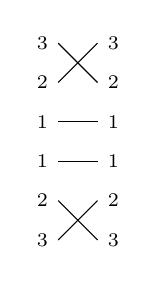
\begin{tikzpicture}[scale=.5,baseline=0]
  \node at (-.9,2.5) {$\scriptstyle 3$};
  \node at (-.9,1.5) {$\scriptstyle 2$};
  \node at (-.9,0.5) {$\scriptstyle 1$};
  \node at (0.9,2.5) {$\scriptstyle 3$};
  \node at (0.9,1.5) {$\scriptstyle 2$};
  \node at (0.9,0.5) {$\scriptstyle 1$};
  \node at (-.9,-2.5) {$\scriptstyle {\ol 3}$};
  \node at (-.9,-1.5) {$\scriptstyle {\ol 2}$};
  \node at (-.9,-0.5) {$\scriptstyle {\ol 1}$};
  \node at (0.9,-2.5) {$\scriptstyle {\ol 3}$};
  \node at (0.9,-1.5) {$\scriptstyle {\ol 2}$};
  \node at (0.9,-0.5) {$\scriptstyle {\ol 1}$};
\draw[-] (-.5,2.5) -- (.5,1.5);
\draw[-] (-.5,1.5) -- (.5,2.5);
\draw[-] (-.5,0.5) -- (.5,0.5);
\draw[-] (-.5,-0.5) -- (.5,-0.5);
\draw[-] (-.5,-1.5) -- (.5,-2.5);
\draw[-] (-.5,-2.5) -- (.5,-1.5);
\end{tikzpicture}
\ntnsp,\quad
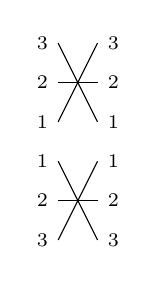
\begin{tikzpicture}[scale=.5,baseline=0]
  \node at (-.9,2.5) {$\scriptstyle 3$};
  \node at (-.9,1.5) {$\scriptstyle 2$};
  \node at (-.9,0.5) {$\scriptstyle 1$};
  \node at (0.9,2.5) {$\scriptstyle 3$};
  \node at (0.9,1.5) {$\scriptstyle 2$};
  \node at (0.9,0.5) {$\scriptstyle 1$};
  \node at (-.9,-2.5) {$\scriptstyle {\ol 3}$};
  \node at (-.9,-1.5) {$\scriptstyle {\ol 2}$};
  \node at (-.9,-0.5) {$\scriptstyle {\ol 1}$};
  \node at (0.9,-2.5) {$\scriptstyle {\ol 3}$};
  \node at (0.9,-1.5) {$\scriptstyle {\ol 2}$};
  \node at (0.9,-0.5) {$\scriptstyle {\ol 1}$};
\draw[-] (-.5,2.5) -- (.5,0.5);
\draw[-] (-.5,1.5) -- (.5,1.5);
\draw[-] (-.5,0.5) -- (.5,2.5);
\draw[-] (-.5,-0.5) -- (.5,-2.5);
\draw[-] (-.5,-1.5) -- (.5,-1.5);
\draw[-] (-.5,-2.5) -- (.5,-0.5);
\end{tikzpicture}
\ntnsp,\quad
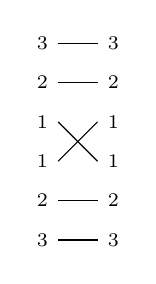
\begin{tikzpicture}[scale=.5,baseline=0]
  \node at (-.9,2.5) {$\scriptstyle 3$};
  \node at (-.9,1.5) {$\scriptstyle 2$};
  \node at (-.9,0.5) {$\scriptstyle 1$};
  \node at (0.9,2.5) {$\scriptstyle 3$};
  \node at (0.9,1.5) {$\scriptstyle 2$};
  \node at (0.9,0.5) {$\scriptstyle 1$};
  \node at (-.9,-2.5) {$\scriptstyle {\ol 3}$};
  \node at (-.9,-1.5) {$\scriptstyle {\ol 2}$};
  \node at (-.9,-0.5) {$\scriptstyle {\ol 1}$};
  \node at (0.9,-2.5) {$\scriptstyle {\ol 3}$};
  \node at (0.9,-1.5) {$\scriptstyle {\ol 2}$};
  \node at (0.9,-0.5) {$\scriptstyle {\ol 1}$};
\draw[-] (-.5,2.5) -- (.5,2.5);
\draw[-] (-.5,1.5) -- (.5,1.5);
\draw[-] (-.5,0.5) -- (.5,-0.5);
\draw[-] (-.5,-0.5) -- (.5,0.5);
\draw[-] (-.5,-1.5) -- (.5,-1.5);
\draw[-] (-.5,-2.5) -- (.5,-2.5);
\end{tikzpicture}
\ntnsp,\quad
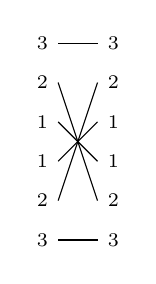
\begin{tikzpicture}[scale=.5,baseline=0]
  \node at (-.9,2.5) {$\scriptstyle 3$};
  \node at (-.9,1.5) {$\scriptstyle 2$};
  \node at (-.9,0.5) {$\scriptstyle 1$};
  \node at (0.9,2.5) {$\scriptstyle 3$};
  \node at (0.9,1.5) {$\scriptstyle 2$};
  \node at (0.9,0.5) {$\scriptstyle 1$};
  \node at (-.9,-2.5) {$\scriptstyle {\ol 3}$};
  \node at (-.9,-1.5) {$\scriptstyle {\ol 2}$};
  \node at (-.9,-0.5) {$\scriptstyle {\ol 1}$};
  \node at (0.9,-2.5) {$\scriptstyle {\ol 3}$};
  \node at (0.9,-1.5) {$\scriptstyle {\ol 2}$};
  \node at (0.9,-0.5) {$\scriptstyle {\ol 1}$};
\draw[-] (-.5,2.5) -- (.5,2.5);
\draw[-] (-.5,1.5) -- (.5,-1.5);
\draw[-] (-.5,0.5) -- (.5,-0.5);
\draw[-] (-.5,-0.5) -- (.5,0.5);
\draw[-] (-.5,-1.5) -- (.5,1.5);
\draw[-] (-.5,-2.5) -- (.5,-2.5);
\end{tikzpicture}
\ntnsp,\quad
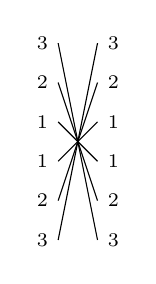
\begin{tikzpicture}[scale=.5,baseline=0]
  \node at (-.9,2.5) {$\scriptstyle 3$};
  \node at (-.9,1.5) {$\scriptstyle 2$};
  \node at (-.9,0.5) {$\scriptstyle 1$};
  \node at (0.9,2.5) {$\scriptstyle 3$};
  \node at (0.9,1.5) {$\scriptstyle 2$};
  \node at (0.9,0.5) {$\scriptstyle 1$};
  \node at (-.9,-2.5) {$\scriptstyle {\ol 3}$};
  \node at (-.9,-1.5) {$\scriptstyle {\ol 2}$};
  \node at (-.9,-0.5) {$\scriptstyle {\ol 1}$};
  \node at (0.9,-2.5) {$\scriptstyle {\ol 3}$};
  \node at (0.9,-1.5) {$\scriptstyle {\ol 2}$};
  \node at (0.9,-0.5) {$\scriptstyle {\ol 1}$};
\draw[-] (-.5,2.5) -- (.5,-2.5);
\draw[-] (-.5,1.5) -- (.5,-1.5);
\draw[-] (-.5,0.5) -- (.5,-0.5);
\draw[-] (-.5,-0.5) -- (.5,0.5);
\draw[-] (-.5,-1.5) -- (.5,1.5);
\draw[-] (-.5,-2.5) -- (.5,2.5);
\end{tikzpicture}
\ntksp ,
\end{equation}
correspond to the reversals
$s'_\emptyset$, $s'_{[1,2]}$, $s'_{[2,3]}$, $s'_{[1,3]}$, $s'_{[\ol1,1]}$, $s'_{[\ol2,2]}$,
$s'_{[\ol3,3]}$.
We refer to all iterations of concatenations and condensed concatenations
of type-$\msfBC$ simple star networks as {\em type-$\msfBC$ star networks},
and let $\net{BC}{[\ol n,n]}$ denote the set of these having boundary
vertices indexed by $[\ol n,n]$.
We will be interested in three subsets of these formed
by condensed concatenation of type-$\msfBC$ simple star networks.

\begin{defn}\label{d:bcstarnet}
  Define $\snet{BC}{[\ol n, n]}$ to be
  the set of all type-$\msfA$ condensed star networks of the form
\begin{equation}\label{eq:bcbulletconcat}
  F = F'_{[c_1,d_1]} \bullet \cdots \bullet F'_{[c_t,d_t]}
  \end{equation}
and call these
{\em type-$\msfBC$ condensed star networks
  (with boundary vertices indexed by $[\ol n,n]$)}.
\end{defn}
\begin{defn}\label{d:bczzn}
Call a type-$\msfBC$ condensed star network $F$ \eqref{eq:bcbulletconcat} a
{\em type-$\msfBC$ zig-zag network} if
the intervals $[c_1,d_1],\dotsc,[c_t,d_t]$
satisfy the conditions of Definition~\ref{d:zz},
i.e. if the type-$\msfA$ star network
$F_{[c_1,d_1]} \bullet \cdots \bullet F_{[c_t,d_t]}$
is a type-$\msfA$ zig-zag network with boundary vertices indexed by
$[ \min\{1,c_1,\dotsc,c_t\}, n]$.
Let $\znet{BC}{[\ol n,n]}$
denote the set of type-$\msfBC$ zig-zag networks with boundary vertices
labeled by $[\ol n,n]$.
\end{defn}
\begin{defn}\label{d:bcdsn}
Call a type-$\msfBC$ star network $F$ \eqref{eq:bcbulletconcat} a
{\em type-$\msfBC$ descending star network} if
the intervals $[c_1,d_1],\dotsc,[c_t,d_t]$
satisfy the conditions of Definition~\ref{d:adsn},
i.e. if the type-$\msfA$ star network
$F_{[c_1,d_1]} \bullet \cdots \bullet F_{[c_t,d_t]}$
is a type-$\msfA$ descending star network with boundary vertices indexed by
$[ \min\{1, c_1,\dotsc,c_t\}, n]$.
Let $\dnet{BC}{[\ol n,n]}$
denote the set of type-$\msfBC$ descending star
networks with boundary vertices
labeled by $[\ol n,n]$.
\end{defn}
Thus we have $\dnet{BC}{[\ol n,n]} \subseteq \znet{BC}{[\ol n,n]}
\subseteq \znet{A}{[\ol n,n]},$
and each zig-zag network of type $\msfBC$
is $F_w$ for some $w \in \mfs{[\ol n, n]}$.
By the symmetry of these networks, we necessarily have $w \in \bn$. 

To illustrate, consider the set $\znet{BC}{[\ol3,3]}$
of twenty-two type-$\msfBC$ zig-zag networks.
Fourteen of these
are type-$\msfBC$ descending star networks
\begin{equation}\label{eq:bcdsn}
\begin{gathered}
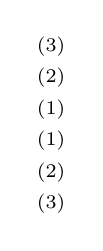
\begin{tikzpicture}[scale=.4,baseline=0]%e
\node at (0,2.5) {$\scriptstyle (3)$};
\node at (0,1.5) {$\scriptstyle (2)$};
\node at (0,0.5) {$\scriptstyle (1)$};
\node at (0,-0.5) {$\scriptstyle (\ol1)$};
\node at (0,-1.5) {$\scriptstyle (\ol2)$};
\node at (0,-2.5) {$\scriptstyle (\ol3)$};
\end{tikzpicture}
  \quad
\begin{tikzpicture}[scale=.4,baseline=0]%e
\draw[-] (-.5,2.5) -- (.5,2.5);
\draw[-] (-.5,1.5) -- (.5,1.5);
\draw[-] (-.5,0.5) -- (.5,0.5);
\draw[-] (-.5,-0.5) -- (.5,-0.5);
\draw[-] (-.5,-1.5) -- (.5,-1.5);
\draw[-] (-.5,-2.5) -- (.5,-2.5);
\node at (0,-4.5) {$F_{123}$};
\node at (0,-5.5) {$\phantom{F_{123}}$};
\end{tikzpicture}
\nTksp ,\ntnsp
\quad
\begin{tikzpicture}[scale=.4,baseline=0]%s0
\draw[-] (-.5,2.5) -- (.5,2.5);
\draw[-] (-.5,1.5) -- (.5,1.5);
\draw[-] (-.5,0.5) -- (.5,-0.5);
\draw[-] (-.5,-0.5) -- (.5,0.5);
\draw[-] (-.5,-1.5) -- (.5,-1.5);
\draw[-] (-.5,-2.5) -- (.5,-2.5);
\node at (0,-4.5) {$F_{\ol123}$};            
\end{tikzpicture}
\nTksp ,\ntnsp
\quad
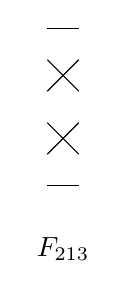
\begin{tikzpicture}[scale=.4,baseline=0]%s1
\draw[-] (-.5,2.5) -- (.5,2.5);
\draw[-] (-.5,1.5) -- (.5,0.5);
\draw[-] (-.5,0.5) -- (.5,1.5);
\draw[-] (-.5,-0.5) -- (.5,-1.5);
\draw[-] (-.5,-1.5) -- (.5,-0.5);
\draw[-] (-.5,-2.5) -- (.5,-2.5);
\node at (0,-4.5) {$F_{213}$};
\end{tikzpicture}
\nTksp ,\ntnsp
\quad
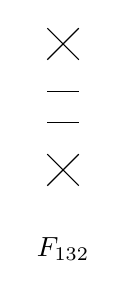
\begin{tikzpicture}[scale=.4,baseline=0]%s2
\draw[-] (-.5,2.5) -- (.5,1.5);
\draw[-] (-.5,1.5) -- (.5,2.5);
\draw[-] (-.5,0.5) -- (.5,0.5);
\draw[-] (-.5,-0.5) -- (.5,-0.5);
\draw[-] (-.5,-1.5) -- (.5,-2.5);
\draw[-] (-.5,-2.5) -- (.5,-1.5);
\node at (0,-4.5) {$F_{132}$};
\end{tikzpicture}
\nTksp ,\;
\quad
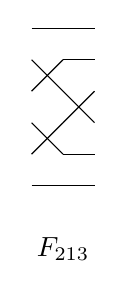
\begin{tikzpicture}[scale=.4,baseline=0]%s1s0
\draw[-] (-.5,2.5) -- (.5,2.5);
\draw[-] (-.5,1.5) -- (.5,0.5);
\draw[-] (-.5,0.5) -- (.5,1.5);
\draw[-] (-.5,-0.5) -- (.5,-1.5);
\draw[-] (-.5,-1.5) -- (.5,-0.5);
\draw[-] (-.5,-2.5) -- (.5,-2.5);
\draw[-] (.5,2.5) -- (1.5,2.5);
\draw[-] (.5,1.5) -- (1.5,1.5);
\draw[-] (.5,0.5) -- (1.5,-0.5);
\draw[-] (.5,-0.5) -- (1.5,0.5);
\draw[-] (.5,-1.5) -- (1.5,-1.5);
\draw[-] (.5,-2.5) -- (1.5,-2.5);
\node at (0.5,-4.5) {$F_{2\ol13}$};
\end{tikzpicture}
\,,
\quad
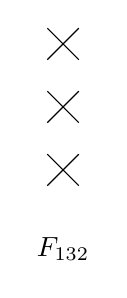
\begin{tikzpicture}[scale=.4,baseline=0]%s2s0
\draw[-] (-.5,2.5) -- (.5,1.5);
\draw[-] (-.5,1.5) -- (.5,2.5);
\draw[-] (-.5,0.5) -- (.5,-0.5);
\draw[-] (-.5,-0.5) -- (.5,0.5);
\draw[-] (-.5,-1.5) -- (.5,-2.5);
\draw[-] (-.5,-2.5) -- (.5,-1.5);
\node at (0,-4.5) {$F_{\ol132}$};
\end{tikzpicture}
\nTksp ,\;\;
\quad
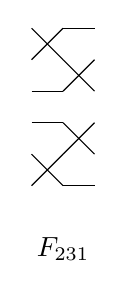
\begin{tikzpicture}[scale=.4,baseline=0]%s2s1
\draw[-] (-.5,2.5) -- (.5,1.5);
\draw[-] (-.5,1.5) -- (.5,2.5);
\draw[-] (-.5,0.5) -- (.5,0.5);
\draw[-] (-.5,-0.5) -- (.5,-0.5);
\draw[-] (-.5,-1.5) -- (.5,-2.5);
\draw[-] (-.5,-2.5) -- (.5,-1.5);
\draw[-] (.5,2.5) -- (1.5,2.5);
\draw[-] (.5,1.5) -- (1.5,0.5);
\draw[-] (.5,0.5) -- (1.5,1.5);
\draw[-] (.5,-0.5) -- (1.5,-1.5);
\draw[-] (.5,-1.5) -- (1.5,-0.5);
\draw[-] (.5,-2.5) -- (1.5,-2.5);
\node at (0.5,-4.5) {$F_{231}$};
\end{tikzpicture} 
\,,
\quad
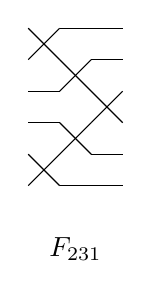
\begin{tikzpicture}[scale=.4,baseline=0]%s2s1s0
\draw[-] (-.5,2.5) -- (.5,1.5);
\draw[-] (-.5,1.5) -- (.5,2.5);
\draw[-] (-.5,0.5) -- (.5,0.5);
\draw[-] (-.5,-0.5) -- (.5,-0.5);
\draw[-] (-.5,-1.5) -- (.5,-2.5);
\draw[-] (-.5,-2.5) -- (.5,-1.5);
\draw[-] (.5,2.5) -- (1.5,2.5);
\draw[-] (.5,1.5) -- (1.5,0.5);
\draw[-] (.5,0.5) -- (1.5,1.5);
\draw[-] (.5,-0.5) -- (1.5,-1.5);
\draw[-] (.5,-1.5) -- (1.5,-0.5);
\draw[-] (.5,-2.5) -- (1.5,-2.5);
\draw[-] (1.5,2.5) -- (2.5,2.5);
\draw[-] (1.5,1.5) -- (2.5,1.5);
\draw[-] (1.5,0.5) -- (2.5,-0.5);
\draw[-] (1.5,-0.5) -- (2.5,0.5);
\draw[-] (1.5,-1.5) -- (2.5,-1.5);
\draw[-] (1.5,-2.5) -- (2.5,-2.5);
\node at (1,-4.5) {$F_{23\ol1}$};
\end{tikzpicture} 
\,,
\\
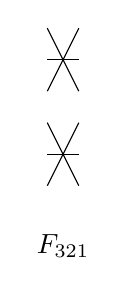
\begin{tikzpicture}[scale=.4,baseline=0]%s13
\draw[-] (-.5,2.5) -- (.5,0.5);
\draw[-] (-.5,1.5) -- (.5,1.5);
\draw[-] (-.5,0.5) -- (.5,2.5);
\draw[-] (-.5,-0.5) -- (.5,-2.5);
\draw[-] (-.5,-1.5) -- (.5,-1.5);
\draw[-] (-.5,-2.5) -- (.5,-0.5);
\node at (0,-4.42) {$F_{321}$};
\end{tikzpicture}
\nTksp, \;\,
\quad
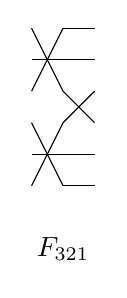
\begin{tikzpicture}[scale=.4,baseline=0]%s13s0
\draw[-] (-.5,2.5) -- (.5,0.5);
\draw[-] (-.5,1.5) -- (.5,1.5);
\draw[-] (-.5,0.5) -- (.5,2.5);
\draw[-] (-.5,-0.5) -- (.5,-2.5);
\draw[-] (-.5,-1.5) -- (.5,-1.5);
\draw[-] (-.5,-2.5) -- (.5,-0.5);
\draw[-] (.5,2.5) -- (1.5,2.5);
\draw[-] (.5,1.5) -- (1.5,1.5);
\draw[-] (.5,0.5) -- (1.5,-0.5);
\draw[-] (.5,-0.5) -- (1.5,0.5);
\draw[-] (.5,-1.5) -- (1.5,-1.5);
\draw[-] (.5,-2.5) -- (1.5,-2.5);
\node at (0.5,-4.5) {$F_{32\ol 1}$};
\end{tikzpicture}
, 
\quad
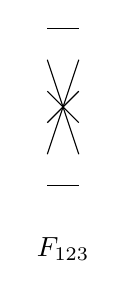
\begin{tikzpicture}[scale=.4,baseline=0]%s22
\draw[-] (-.5,2.5) -- (.5,2.5);
\draw[-] (-.5,1.5) -- (.5,-1.5);
\draw[-] (-.5,0.5) -- (.5,-0.5);
\draw[-] (-.5,-0.5) -- (.5,0.5);
\draw[-] (-.5,-1.5) -- (.5,1.5);
\draw[-] (-.5,-2.5) -- (.5,-2.5);
\node at (0,-4.5) {$F_{\ol1\ol23}$};
\end{tikzpicture}
\nTksp , \;
\quad
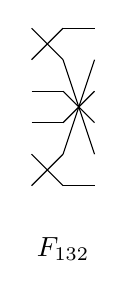
\begin{tikzpicture}[scale=.4,baseline=0]%s2s22
\draw[-] (-.5,2.5) -- (.5,1.5);
\draw[-] (-.5,1.5) -- (.5,2.5);
\draw[-] (-.5,0.5) -- (.5,0.5);
\draw[-] (-.5,-0.5) -- (.5,-0.5);
\draw[-] (-.5,-1.5) -- (.5,-2.5);
\draw[-] (-.5,-2.5) -- (.5,-1.5);
\draw[-] (.5,2.5) -- (1.5,2.5);
\draw[-] (.5,1.5) -- (1.5,-1.5);
\draw[-] (.5,0.5) -- (1.5,-0.5);
\draw[-] (.5,-0.5) -- (1.5,0.5);
\draw[-] (.5,-1.5) -- (1.5,1.5);
\draw[-] (.5,-2.5) -- (1.5,-2.5);
\node at (0.5,-4.5) {$F_{\ol13\ol2}$};
\end{tikzpicture}
,\;
\quad
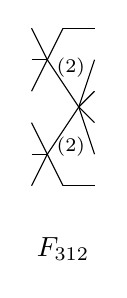
\begin{tikzpicture}[scale=.4,baseline=0]%s13s22
\draw[-] (-1,2.5) -- (-.5,1.5); \draw[-] (-.5,1.5) -- (0,2.5);
\draw[-] (-1,1.5) -- (-.5,1.5); \draw[-] (-.5,1.5) -- (.5,0);
\draw[-] (-1,0.5) -- (-.5,1.5);
\draw[-] (-1,-0.5) -- (-.5,-1.5); \draw[-] (-.5,-1.5) -- (.5,0);
\draw[-] (-1,-1.5) -- (-.5,-1.5); \draw[-] (-.5,-1.5) -- (0,-2.5);
\draw[-] (-1,-2.5) -- (-.5,-1.5);
\draw[-] (0,2.5) -- (1,2.5);
\draw[-] (.5,0) -- (1,1.5);
\draw[-] (.5,0) -- (1,0.5);
\draw[-] (.5,0) -- (1,-0.5);
\draw[-] (.5,0) -- (1,-1.5);
\draw[-] (0,-2.5) -- (1,-2.5);
\node at (0.25,1.25) {$\scriptstyle (2)$};
\node at (0.25,-1.25) {$\scriptstyle (2)$};
\node at (0,-4.5) {$F_{3\ol1\ol2}$};
\end{tikzpicture}
,
\quad
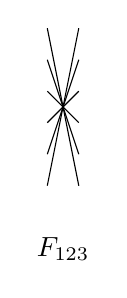
\begin{tikzpicture}[scale=.4,baseline=0]%s33
\draw[-] (-.5,2.5) -- (.5,-2.5);
\draw[-] (-.5,1.5) -- (.5,-1.5);
\draw[-] (-.5,0.5) -- (.5,-0.5);
\draw[-] (-.5,-0.5) -- (.5,0.5);
\draw[-] (-.5,-1.5) -- (.5,1.5);
\draw[-] (-.5,-2.5) -- (.5,2.5);
\node at (0,-4.5) {$F_{\ol1\ol2\ol3}$};
\end{tikzpicture}
\nTksp,
\end{gathered}
\end{equation}
and eight are not,
\begin{equation}\label{eq:bczznotdsn}        
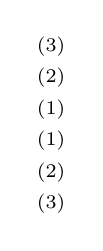
\begin{tikzpicture}[scale=.4,baseline=0]%e
\node at (0,2.5) {$\scriptstyle (3)$};
\node at (0,1.5) {$\scriptstyle (2)$};
\node at (0,0.5) {$\scriptstyle (1)$};
\node at (0,-0.5) {$\scriptstyle (\ol1)$};
\node at (0,-1.5) {$\scriptstyle (\ol2)$};
\node at (0,-2.5) {$\scriptstyle (\ol3)$};
\end{tikzpicture} \quad
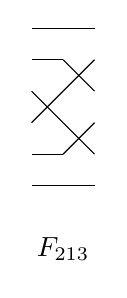
\begin{tikzpicture}[scale=.4,baseline=0]%s0s1
\draw[-] (-.5,2.5) -- (.5,2.5);
\draw[-] (-.5,1.5) -- (.5,1.5);
\draw[-] (-.5,0.5) -- (.5,-0.5);
\draw[-] (-.5,-0.5) -- (.5,0.5);
\draw[-] (-.5,-1.5) -- (.5,-1.5);
\draw[-] (-.5,-2.5) -- (.5,-2.5);
\draw[-] (.5,2.5) -- (1.5,2.5);
\draw[-] (.5,1.5) -- (1.5,0.5);
\draw[-] (.5,0.5) -- (1.5,1.5);
\draw[-] (.5,-0.5) -- (1.5,-1.5);
\draw[-] (.5,-1.5) -- (1.5,-0.5);
\draw[-] (.5,-2.5) -- (1.5,-2.5);
\node at (0.5,-4.5) {$F_{\ol213}$};
\end{tikzpicture}
,\quad
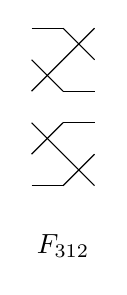
\begin{tikzpicture}[scale=.4,baseline=0]%s1s2
\draw[-] (-.5,2.5) -- (.5,2.5);
\draw[-] (-.5,1.5) -- (.5,0.5);
\draw[-] (-.5,0.5) -- (.5,1.5);
\draw[-] (-.5,-0.5) -- (.5,-1.5);
\draw[-] (-.5,-1.5) -- (.5,-0.5);
\draw[-] (-.5,-2.5) -- (.5,-2.5);
\draw[-] (.5,2.5) -- (1.5,1.5);
\draw[-] (.5,1.5) -- (1.5,2.5);
\draw[-] (.5,0.5) -- (1.5,0.5);
\draw[-] (.5,-0.5) -- (1.5,-0.5);
\draw[-] (.5,-1.5) -- (1.5,-2.5);
\draw[-] (.5,-2.5) -- (1.5,-1.5);
\node at (0.5,-4.42) {$F_{312}$};
\end{tikzpicture}
,\quad
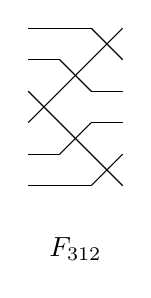
\begin{tikzpicture}[scale=.4,baseline=0]%s0s1s2
\draw[-] (-.5,2.5) -- (.5,2.5);
\draw[-] (-.5,1.5) -- (.5,1.5);
\draw[-] (-.5,0.5) -- (.5,-0.5);
\draw[-] (-.5,-0.5) -- (.5,0.5);
\draw[-] (-.5,-1.5) -- (.5,-1.5);
\draw[-] (-.5,-2.5) -- (.5,-2.5);
\draw[-] (.5,2.5) -- (1.5,2.5);
\draw[-] (.5,1.5) -- (1.5,0.5);
\draw[-] (.5,0.5) -- (1.5,1.5);
\draw[-] (.5,-0.5) -- (1.5,-1.5);
\draw[-] (.5,-1.5) -- (1.5,-0.5);
\draw[-] (.5,-2.5) -- (1.5,-2.5);
\draw[-] (1.5,2.5) -- (2.5,1.5);
\draw[-] (1.5,1.5) -- (2.5,2.5);
\draw[-] (1.5,0.5) -- (2.5,0.5);
\draw[-] (1.5,-0.5) -- (2.5,-0.5);
\draw[-] (1.5,-1.5) -- (2.5,-2.5);
\draw[-] (1.5,-2.5) -- (2.5,-1.5);
\node at (1,-4.5) {$F_{\ol312}$};
\end{tikzpicture}
,\quad
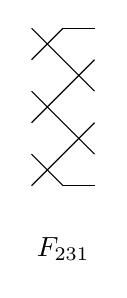
\begin{tikzpicture}[scale=.4,baseline=0]%s2s0s1
\draw[-] (-.5,2.5) -- (.5,1.5);
\draw[-] (-.5,1.5) -- (.5,2.5);
\draw[-] (-.5,0.5) -- (.5,-0.5);
\draw[-] (-.5,-0.5) -- (.5,0.5);
\draw[-] (-.5,-1.5) -- (.5,-2.5);
\draw[-] (-.5,-2.5) -- (.5,-1.5);
\draw[-] (.5,2.5) -- (1.5,2.5);
\draw[-] (.5,1.5) -- (1.5,0.5);
\draw[-] (.5,0.5) -- (1.5,1.5);
\draw[-] (.5,-0.5) -- (1.5,-1.5);
\draw[-] (.5,-1.5) -- (1.5,-0.5);
\draw[-] (.5,-2.5) -- (1.5,-2.5);
\node at (0.5,-4.5) {$F_{\ol231}$};
\end{tikzpicture}
,\quad
\begin{tikzpicture}[scale=.4,baseline=0]%s1s0s2
\draw[-] (-.5,2.5) -- (.5,2.5);
\draw[-] (-.5,1.5) -- (.5,0.5);
\draw[-] (-.5,0.5) -- (.5,1.5);
\draw[-] (-.5,-0.5) -- (.5,-1.5);
\draw[-] (-.5,-1.5) -- (.5,-0.5);
\draw[-] (-.5,-2.5) -- (.5,-2.5);
\draw[-] (.5,2.5) -- (1.5,1.5);
\draw[-] (.5,1.5) -- (1.5,2.5);
\draw[-] (.5,0.5) -- (1.5,-0.5);
\draw[-] (.5,-0.5) -- (1.5,0.5);
\draw[-] (.5,-1.5) -- (1.5,-2.5);
\draw[-] (.5,-2.5) -- (1.5,-1.5);
\node at (0.5,-4.5) {$F_{3\ol12}$};
\end{tikzpicture}
,\quad
\begin{tikzpicture}[scale=.4,baseline=0]%s0s13
\draw[-] (-.5,2.5) -- (.5,2.5);
\draw[-] (-.5,1.5) -- (.5,1.5);
\draw[-] (-.5,0.5) -- (.5,-0.5);
\draw[-] (-.5,-0.5) -- (.5,0.5);
\draw[-] (-.5,-1.5) -- (.5,-1.5);
\draw[-] (-.5,-2.5) -- (.5,-2.5);
\draw[-] (.5,2.5) -- (1.5,0.5);
\draw[-] (.5,1.5) -- (1.5,1.5);
\draw[-] (.5,0.5) -- (1.5,2.5);
\draw[-] (.5,-0.5) -- (1.5,-2.5);
\draw[-] (.5,-1.5) -- (1.5,-1.5);
\draw[-] (.5,-2.5) -- (1.5,-0.5);
\node at (0.5,-4.5) {$F_{\ol321}$};
\end{tikzpicture}
,\quad
\begin{tikzpicture}[scale=.4,baseline=0]%s22s2
\draw[-] (-.5,2.5) -- (.5,2.5);
\draw[-] (-.5,1.5) -- (.5,-1.5);
\draw[-] (-.5,0.5) -- (.5,-0.5);
\draw[-] (-.5,-0.5) -- (.5,0.5);
\draw[-] (-.5,-1.5) -- (.5,1.5);
\draw[-] (-.5,-2.5) -- (.5,-2.5);
\draw[-] (.5,2.5) -- (1.5,1.5);
\draw[-] (.5,1.5) -- (1.5,2.5);
\draw[-] (.5,0.5) -- (1.5,0.5);
\draw[-] (.5,-0.5) -- (1.5,-0.5);
\draw[-] (.5,-1.5) -- (1.5,-2.5);
\draw[-] (.5,-2.5) -- (1.5,-1.5);
\node at (0.5,-4.5) {$F_{\ol1\ol32}$};
\end{tikzpicture}
,\quad
\begin{tikzpicture}[scale=.4,baseline=0]%s22s13
\draw[-] (1,2.5) -- (.5,1.5); \draw[-] (.5,1.5) -- (0,2.5);
\draw[-] (1,1.5) -- (.5,1.5); \draw[-] (.5,1.5) -- (-.5,0);
\draw[-] (1,0.5) -- (.5,1.5);
\draw[-] (1,-0.5) -- (.5,-1.5); \draw[-] (.5,-1.5) -- (-.5,0);
\draw[-] (1,-1.5) -- (.5,-1.5); \draw[-] (.5,-1.5) -- (0,-2.5);
\draw[-] (1,-2.5) -- (.5,-1.5);
\draw[-] (0,2.5) -- (-1,2.5);
\draw[-] (-.5,0) -- (-1,1.5);
\draw[-] (-.5,0) -- (-1,0.5);
\draw[-] (-.5,0) -- (-1,-0.5);
\draw[-] (-.5,0) -- (-1,-1.5);
\draw[-] (0,-2.5) -- (-1,-2.5);
\node at (-0.25,1.25) {$\scriptstyle (2)$};
\node at (-0.25,-1.25) {$\scriptstyle (2)$};
\node at (0,-4.5) {$F_{\ol3\ol21}$};
\end{tikzpicture}
.
\end{equation}

By Corollary~\ref{c:atmostonepath} and the containment
$\bn \subseteq \snn$, we have that
for all $F_w \in \znet{BC}{[\ol n ,n]}$ and $v \in \bn$,
at most one
path family $\pi$ of type $v$
covers $F_w$.
For $i>0$, paths $\pi_i$ and $\pi_{\ol i}$ in this family
are necessarily mirror
images of one another, and we call $\pi_i$
{\em grounded} if it intersects path $\pi_{\ol i}$.
For example consider $F_{3\ol12}$ in \eqref{eq:bczznotdsn}
and the path families
$\pi$ of type $123$ and $\sigma$ of type $3\ol12$ covering it,
\begin{equation}\label{eq:pisigma}
  \pi = 
\begin{tikzpicture}[scale=.4,baseline=0]%s1s0s2
  \node at (-.9,2.5) {$\scriptstyle 3$};
  \node at (-.9,1.5) {$\scriptstyle 2$};
  \node at (-.9,0.5) {$\scriptstyle 1$};
  \node at (1.9,2.5) {$\scriptstyle 3$};
  \node at (1.9,1.5) {$\scriptstyle 2$};
  \node at (1.9,0.5) {$\scriptstyle 1$};
  \node at (-.9,-2.5) {$\scriptstyle {\ol 3}$};
  \node at (-.9,-1.5) {$\scriptstyle {\ol 2}$};
  \node at (-.9,-0.5) {$\scriptstyle {\ol 1}$};
  \node at (1.9,-2.5) {$\scriptstyle {\ol 3}$};
  \node at (1.9,-1.5) {$\scriptstyle {\ol 2}$};
  \node at (1.9,-0.5) {$\scriptstyle {\ol 1}$};
  \draw[-, very thick]
  (-.5,2.5) -- (.5,2.5) -- (1,2) -- (1.5,2.5);
  \draw[-, dotted, very thick]
  (-.5,1.5) -- (0,1) -- (.5,1.5) -- (1,2) -- (1.5,1.5);
  \draw[-, dashed, very thick]
  (-.5,0.5) -- (0,1) -- (.5,0.5) -- (1,0) -- (1.5,0.5);
  \draw[-, thin]
  (-.5,-0.43) -- (0,-.93) -- (.5,-0.43) -- (1,0.07) -- (1.5,-0.43);
  \draw[-, thin]
  (-.5,-0.57) -- (0,-1.07) -- (.5,-0.57) -- (1,-0.07) -- (1.5,-0.57);
  \draw[-, dotted, thick]
  (-.5,-1.5) -- (0,-1) -- (.5,-1.5) -- (1,-2) -- (1.5,-1.5);
  \draw[-]
  (-.5,-2.5) -- (.5,-2.5) -- (1,-2) -- (1.5,-2.5);
\end{tikzpicture}\, ,
  \qquad \qquad
  \sigma = \begin{tikzpicture}[scale=.4,baseline=0]%s1s0s2
  \node at (-.9,2.5) {$\scriptstyle 3$};
  \node at (-.9,1.5) {$\scriptstyle 2$};
  \node at (-.9,0.5) {$\scriptstyle 1$};
  \node at (1.9,2.5) {$\scriptstyle 3$};
  \node at (1.9,1.5) {$\scriptstyle 2$};
  \node at (1.9,0.5) {$\scriptstyle 1$};
  \node at (-.9,-2.5) {$\scriptstyle {\ol 3}$};
  \node at (-.9,-1.5) {$\scriptstyle {\ol 2}$};
  \node at (-.9,-0.5) {$\scriptstyle {\ol 1}$};
  \node at (1.9,-2.5) {$\scriptstyle {\ol 3}$};
  \node at (1.9,-1.5) {$\scriptstyle {\ol 2}$};
  \node at (1.9,-0.5) {$\scriptstyle {\ol 1}$};
  \draw[-, very thick]
  (-.5,2.5) -- (.5,2.5) -- (1,2) -- (1.5,1.5);
  \draw[-, dotted, very thick]
  (-.5,0.5) -- (0,1) -- (.5,1.5) -- (1,2) -- (1.5,2.5);
  \draw[-, dashed, very thick]
  (-.5,1.5) -- (0,1) -- (.5,0.5) -- (1,0) -- (1.5,-0.5);
  \draw[-]
  (-.5,-2.5) -- (.5,-2.5) -- (1,-2) -- (1.5,-1.5);
  \draw[-, dotted, thick]
  (-.5,-0.5) -- (0,-1) -- (.5,-1.5) -- (1,-2) -- (1.5,-2.5);
  \draw[-, thin]
  (-.5,-1.43) -- (0,-.93) -- (.5,-0.43) -- (1,0.07) -- (1.5,0.57);
  \draw[-, thin]
  (-.5,-1.57) -- (0,-1.07) -- (.5,-0.57) -- (1,-.07) -- (1.5,0.43);
\end{tikzpicture}\, .
\end{equation}
The path $\pi_1$ is grounded while $\pi_2$ and $\pi_3$ are not;
the path $\sigma_2$ is grounded while $\sigma_1$ and $\sigma_3$ are not.

By \eqref{eq:bcstardef} the intervals appearing in the construction
of the type-$\msfBC$ star network $G$ \eqref{eq:bcbulletconcat}
are roughly half of those that appear in the type-$\msfA$ construction
of the same network.  The subposet of $\preceq$ induced by these intervals
satisfies the following.
\begin{prop}\label{p:atmostonesymminterval}
  For $F'_{\smash{[a_1,b_1]}} \bullet \cdots \bullet F'_{\smash{[a_t,b_t]}}$ 
  a type-$\msfBC$ zig-zag network,
  there is at most one interval $[a_i, b_i]$
  satisfying $a_i < 0$, $b_i = \ol{a_i}$.
  Furthermore, this interval is maximal or minimal
  (or both) in the poset $\preceq$ on $\{ [a_1,b_1], \dotsc, [a_t,b_t] \}$.
\end{prop}
\begin{proof}
  Condition (1) of Definition~\ref{d:zz} requires that the intervals
  $[a_1,b_1], \dotsc, [a_t,b_t]$ be distinct and form a nonnesting set.
  Thus at most one of these intervals satisfies $b_i = \ol{a_i}$.
  Let $[a_j,\ol{a_j}]$ be such an interval ($a_j < 0$) and suppose that
  it is neither maximal nor minimal in the partial order $\preceq$.
  Then there are indices $i, k$ with $i < j < k$ and
  $[a_i,b_i] \cap [a_j,\ol{a_j}] \neq \emptyset$,
  $[a_k,b_k] \cap [a_j,\ol{a_j}] \neq \emptyset$.  By Condition (2)
  of Definition~\ref{d:zz}, we must have $a_i < a_j < a_k$
  or $a_i > a_j > a_k$.  But this implies that $a_i < 0$ or $a_k < 0$, and
  therefore that $[a_j, \ol{a_j}]$ is properly contained in $[a_i, \ol{a_i}]$
  or $[a_k,\ol{a_k}]$, contradicting Condition (1).
  \end{proof}
As a consequence, the cardinalities of $\znet{BC}{[\ol n,n]}$ and
$\dnet{BC}{[\ol n,n]}$ are related to their type-$\msfA$ analogs,
with the second cardinality equal to a Catalan number.
\begin{thm}\label{t:catalan}
  For all $n$ we have
  \begin{enumerate}
  \item $|\znet{BC}{[\ol n,n]}| = |\znet{A}{[1,n+1]}|$,
  \item $|\dnet{BC}{[\ol n,n]}| = |\dnet{A}{[1,n+1]}| = \frac1{n+2} \tbinom{2n+2}{n+1}$.
    \end{enumerate}
\end{thm}
\begin{proof}
  (1) Define a map
  $\Upsilon: \znet{BC}{[\ol n, n]} \rightarrow \znet{A}{[1, n+1]}$ by
  $\Upsilon(F'_{[a_i,b_i]}) = F_{[\max\{a_i+1,1\},b_i+1]}$ and
  \begin{equation*}
      \Upsilon(F'_{[a_1,b_1]} \bullet \cdots \bullet F'_{[a_t,b_t]})
      =
    \Upsilon(F'_{[a_1, b_1]}) \bullet \cdots \bullet \Upsilon(F'_{[a_t,b_t]}),
  \end{equation*}
  so that all positive endpoints of intervals increase by one
  and all negative endpoints are replaced by $1$.
  To see that $\Upsilon$ is well defined, recall
  that by Proposition~\ref{p:atmostonesymminterval}
  at most one of the intervals $[a_i,b_i]$ satisfies $a_i < 0$.
  Thus the conditions of Definition~\ref{d:zz} are satisfied
  and $\Upsilon(F)$ belongs to $\znet{A}{[1,n+1]}$.
  Furthermore, for $F \in \dnet{BC}{[\ol n, n]}$,
  the inequalities $a_1 > \cdots > a_t$ imply that we have
  $a_1 + 1 > \cdots > \max\{a_t + 1, 1\}$ and
  $\Upsilon(F) \in \dnet{A}{[1,n+1]}$.
  To see that $\Upsilon$ is bijective, observe that we have
  \begin{equation*}
  \begin{gathered}
    \;[a_i,b_i] \subseteq [1,n] \;\Longleftrightarrow\;
      [a_i+1,b_i+1] \subseteq [2,n+1],\\
  a_i = b_i \in [1,n] \;\Longleftrightarrow\; a_i+1 = b_i+1 \in [2,n+1], \\
  [\ol{b_i},b_i] \subseteq [\ol n, n] \;\Longleftrightarrow\;
  [1,b_i+1] \subseteq [1,n+1].
  \end{gathered}
\end{equation*}
  Finally, by \cite[Thm.\,3.6]{CHSSkanEKL} we have
  $|\dnet{A}{[1,n]}| = \tfrac 1{n+1} \tbinom{2n}n$.
\end{proof}


In Theorems~\ref{t:znetbcpavoid} -- \ref{t:dnetbcpavoid}
we will characterize
$\znet{BC}{[\ol n,n]}$ and $\dnet{BC}{[\ol n,n]}$
as subsets of $\{ F_w \in \znet{A}{[\ol n,n]} \,|\, w \in \bn \}$
defined by $w$ avoiding certain patterns.
In order to do so, we
decompose certain
elements of $\bn$ into pairs $(u,v) \in \mfb k \times \mfs{n-k}$,
and certain
zig-zag networks in $\znet{BC}{[\ol n,n]}$
into pairs of components in $\znet{BC}{[\ol k,k]} \times \znet{A}{[1,n-k]}$.
Define the map
\begin{equation}\label{eq:oplusperm}
  \begin{aligned}
    \oplus: \mfb{k} \times \mfs{[1,n-k]} &\rightarrow \mfb{n}\\
    (u,v) &\mapsto u \oplus v = w_{\ol{n}} \cdots w_{\ol1} w_1 \cdots w_n
  \end{aligned}
\end{equation}
by 
\begin{equation*}
  w_i = \begin{cases}
    u_i &\text{if $i \in [\ol k, k]$},\\
    v_i + k &\text{if $i > k$},\\
    \ol{v_i + k} &\text{if $i < \ol k$}.
  \end{cases}
\end{equation*}
For example,
the elements
$u = \ol 1 \in \mfb1$, $v = 231 \in \mfs3$ give
$u \oplus v  =\ol2\ol4\ol3 1 \ol1 342 \in \mfb4$.
Observe that to make sense of the more general expression
$u \oplus v^{(1)} \oplus \cdots \oplus v^{(p)}$,
we must interpret it as
$( \cdots ((u \oplus v^{(1)}) \oplus v^{(2)}) \oplus \cdots \oplus v^{(p-1)}) \oplus v^{(p)}$, with $u \in \mfb{k}$, $v^{(i)} \in \mfs{[1,j_i]}$
for some $k, j_1, \dotsc, j_p$.
We will say that any element $w \in \bn$ which can be written as
$w = u \oplus v$ is {\em $\oplus$-decomposable}.
Equivalently, $w \in \bn$ is $\oplus$-decomposable if there is
some index $k$ such that
\begin{equation*}
  \{|w_1|, \dotsc, |w_k| \} = [1,k], \qquad \{w_{k+1}, \dotsc, w_n\} = [k+1,n].
\end{equation*}

We define a similar map
\begin{equation}\label{eq:oplusnet}
  \begin{aligned}
    \oplus: \snet{BC}{[\ol k,k]} \times \snet{A}{[1,n-k]} &\rightarrow \snet{BC}{[\ol n,n]}\\
      (E,F) &\mapsto E \oplus F
  \end{aligned}
\end{equation}
as follows.
\begin{enumerate}
\item Create $F^+ \in \snet{A}{[k+1,n]}$ by adding $k$ to the
  indices of all sources and sinks of $F$.
\item Create $F^- \in \snet{A}{[\ol n, \ol{k+1}]}$ by drawing $F^+$ upside-down
  and by multiplying each source and sink index by $-1$.
\item Vertically arrange the sources and sinks of these networks and $E$
  in order $(\ol n, \dotsc, n)$, so that we have $F^+$ above $E$ above $F^-$.
\end{enumerate}
For example, to construct
the network $F'_{[\ol1,1]} \oplus ( F_{[2,3]} \bullet F_{[1,2]} )$,
we place $F'_{[\ol1,1]}$ between
two copies of $F_{[2,3]} \bullet F_{[1,2]}$,
one upside-down,
to obtain
\begin{equation*}
  \begin{aligned}
      &\phantom . \\
  F'_{[\ol1,1]} &=
\begin{tikzpicture}[scale=.5,baseline=-25]
\node at (-.4,-1) {$\scriptstyle 1$};
\node at (-.4,-2) {$\scriptstyle{\ol1}$};
\node at (1.4,-1) {$\scriptstyle 1$};
\node at (1.4,-2) {$\scriptstyle{\ol1}$};
\draw[-] (0,-1) -- (1,-2);
\draw[-] (0,-2) -- (1,-1);
\end{tikzpicture},\\
\\
  F_{[2,3]} \bullet F_{[1,2]} &=
\begin{tikzpicture}[scale=.5,baseline=-18]
\node at (-.4,0)  {$\scriptstyle 3$};
\node at (-.4,-1) {$\scriptstyle 2$};
\node at (-.4,-2) {$\scriptstyle 1$};
\node at (2.4,0)  {$\scriptstyle 3$};
\node at (2.4,-1) {$\scriptstyle 2$};
\node at (2.4,-2) {$\scriptstyle 1$};
\draw[-] (0,0) -- (2,-2);
\draw[-] (0,-1) -- (1,0) -- (2,0);
\draw[-] (0,-2) -- (1,-2) -- (2,-1);
\end{tikzpicture}\ntnsp,
\end{aligned}
  \quad
  F'_{[\ol1,1]} \oplus ( F_{[2,3]} \bullet F_{[1,2]} ) = 
\begin{tikzpicture}[scale=.5,baseline=-5]
  \node at (-.4,3.5) {$\scriptstyle 4$};
  \node at (-.4,2.5) {$\scriptstyle 3$};
  \node at (-.4,1.5) {$\scriptstyle 2$};
  \node at (-.4,0.5) {$\scriptstyle 1$};
  \node at (-.4,-0.5) {$\scriptstyle \ol1$};
  \node at (-.4,-1.5) {$\scriptstyle \ol2$};
  \node at (-.4,-2.5) {$\scriptstyle \ol3$};
  \node at (-.4,-3.5) {$\scriptstyle \ol4$};
  \node at (2.4,3.5) {$\scriptstyle 4$};
  \node at (2.4,2.5) {$\scriptstyle 3$};
  \node at (2.4,1.5) {$\scriptstyle 2$};
  \node at (2.4,0.5) {$\scriptstyle 1$};
  \node at (2.4,-0.5) {$\scriptstyle \ol1$};
  \node at (2.4,-1.5) {$\scriptstyle \ol2$};
  \node at (2.4,-2.5) {$\scriptstyle \ol3$};
  \node at (2.4,-3.5) {$\scriptstyle \ol4$};
\draw[-] (0,3.5) -- (2,1.5);
\draw[-] (0,2.5) -- (1,3.5) -- (2,3.5);
\draw[-] (0,1.5) -- (1,1.5) -- (2,2.5);
\draw[-] (0,0.5) -- (1,-0.5) -- (2,-0.5);
\draw[-] (0,-3.5) -- (2,-1.5);
\draw[-] (0,-2.5) -- (1,-3.5) -- (2,-3.5);
\draw[-] (0,-1.5) -- (1,-1.5) -- (2,-2.5);
\draw[-] (0,-0.5) -- (1,0.5) -- (2,0.5);
\end{tikzpicture}
\cong F'_{[\ol1,1]} \bullet F'_{[2,3]} \bullet F'_{[1,2]}.
\end{equation*}

\begin{lem}\label{l:opluszz}
  For elements $u \in \mfb k$, $v \in \mfs{n-k}$
  and zig-zag networks
  $F_u \in \znet{BC}{[\ol k, k]}$,
  $F_v \in \znet{A}{[1,n-k]}$,
  we have the following.
  \begin{enumerate}
  \item $F_u \oplus F_v \in \znet{BC}{[\ol n, n]}$ is a zig-zag network
    satisfying $w(F_u \oplus F_v) = u \oplus v$.
  \item If $F_u$ and $F_v$ are descending star networks, then so is
    $F_u \oplus F_v$.
  \end{enumerate}
\end{lem}
\begin{proof}
  (1) To see that $F_u \oplus F_v$ belongs to $\znet{BC}{[\ol n, n]}$, write
  \begin{equation*}
      F_u = F'_{[c_1,d_1]} \bullet \cdots \bullet F'_{[c_t,d_t]}, \qquad
      F_v = F_{[a_1,b_1]} \bullet \cdots \bullet F_{[a_r,b_r]}.
  \end{equation*}
  By the definition \eqref{eq:oplusnet} of the map $\oplus$ we have
  \begin{equation*}
    F_u \oplus F_v = F'_{[c_1,d_1]} \bullet \cdots \bullet F'_{[c_t,d_t]}
    \bullet F'_{[a_1+k,b_1+k]} \bullet \cdots \bullet F'_{[a_r+k,b_r+k]}.
  \end{equation*}
  It is easy to see that the set $\{[a_1+k,b_1+k],\dotsc,[a_r+k,b_r+k]\}$
  satisfies the conditions of Definition~\ref{d:zz},
  and since each interval $[c_i,d_i]$ is disjoint
  from each interval $[a_j+k,b_j+k]$, the union
  $\{[c_1,d_1],\dotsc,[c_t,d_t],[a_1+k,b_1+k], \dotsc, [a_r+k,b_r+k]\}$
  satisfies the conditions of Definition~\ref{d:zz} as well.

  Now let $w = w(F_u \oplus F_v) \in \bn$ and let $y = u \oplus v \in \bn$.
  To see that $w = y$,
  recall by Proposition~\ref{p:wFchar}
  that $w$ is the permutation in $\snn$
  which maximizes $\inv(z)$ over all $z \in \snn$
  for which there is a path family of type $z$ covering $F_u \oplus F_v$.
  By the disconnectedness of $F_u \oplus F_v$, we have
  \begin{equation*}
    \{w_{\ol k}, \dotsc, w_k \} = [\ol k, k],
    \qquad
    \ntksp\nhtnsp\{w_{k+1}, \dotsc, w_n \} = [k+1,n],
    \qquad
    \ntksp\nhtnsp\{w_{\ol n}, \dotsc, w_{\ol{k+1}} \} = [\ol n, \ol{k+1}].
  \end{equation*}
  Since $w(F_u) = u$, it is clear that $w$ has as many inversions as possible
  among entries $\ol k, \dotsc, k$ when
  $w_{\ol k} \cdots w_k = u_{\ol k} \cdots u_k$.
  Similarly,
  $w$ has as many inversions as possible
  among entries $k+1, \dotsc, n$ when
  $w_{k+1} \cdots w_n$ matches the pattern $v_1 \cdots v_{n-k}$, i.e.   when $w_{k+i} = v_i + k$ for $i = 1,\dotsc,n-k$.
  In this case,
  we also have
  $w_{\ol n} \cdots w_{\ol{k+1}} = \ol{w_n} \cdots \ol{w_{k+1}}$.
  Thus we have $w = u \oplus v$.

  (2) The fact that $F_u \oplus F_v$ belongs to $\dnet{BC}{[\ol n,n]}$
  follows immediately from Definition~\ref{d:bcdsn}.
\end{proof}


Now we may characterize $\znet{BC}{[\ol n, n]}$ and $\dnet{BC}{[\ol n, n]}$
in terms of pattern avoidance.

\begin{thm}\label{t:znetbcpavoid}
  Elements of $\znet{BC}{[\ol n,n]}$ correspond bijectively to
  \pavoiding elements of $\bn$.  Specifically we have
  \begin{equation}\label{eq:znetbcseteq}
    \znet{BC}{[\ol n, n]} =
    \{ F_w \in \znet{A}{[\ol n,n]} \,|\, w \in \bn \}.
    \end{equation}
\end{thm}
\begin{proof}
  ($\subseteq$)
  Consider $F \in \znet{BC}{[\ol n,n]} \subset \znet{A}{[\ol n,n]}$.
  By \cite[\S 3]{SkanNNDCB}, $F$ has the form $F_w$
  for some $w \in \snn$ \avoidingp, and factors as in
  \eqref{eq:bcbulletconcat}
  and Definition~\ref{d:zz}.
  By Proposition~\ref{p:atmostonesymminterval},
  at most one of the intervals $[c_i,d_i]$ appearing in
  \eqref{eq:bcbulletconcat} satisfies $c_i = \ol{d_i}$.
  If such an interval exists, then we may assume that it appears
  first or last.
  Thus we may factor $F$ as
  \begin{equation*}
    F'_{[c_0,d_0]} \bullet
    (F'_{[c_1,d_1]} \bullet F'_{[\ol{d_1},\ol{c_1}]}) \bullet \cdots \bullet
    (F'_{[c_t,d_t]} \bullet F'_{[\ol{d_t},\ol{c_t}]})
    \bullet F'_{[c_{t+1},d_{t+1}]},
  \end{equation*}
  with one or both of the intervals $[c_0,d_0]$ and $[c_{t+1},d_{t+1}]$
  satisfying $c_i=d_i$, and at most one of these satisfying $c_i = \ol{d_i}$.
  Algorithm~\ref{a:FwF}
  then gives a reversal factorization of $w$.
  This factorization consists of the subsequence of reversals
  \begin{equation}\label{eq:mainreversals}
    (s_{[c_0,d_0]}, s_{[c_1,d_1]}, s_{[\ol{d_1},\ol{c_1}]}, \dotsc,
    s_{[c_t,d_t]}, s_{[\ol{d_t},\ol{c_t}]}, s_{[\ol{d_{t+1}},\ol{c_{t+1}}]}),
  \end{equation}
  and more pairs of reversals 
  \begin{equation}\label{eq:intreversals}
    s_{[c_i,d_i] \cap [c_j,d_j]}, \quad  s_{[\ol{d_i},\ol{c_i}] \cap [\ol{d_j},\ol{c_j}]}
  \end{equation}
  inserted between these.
  Since the only intervals appearing in
  \eqref{eq:mainreversals}) -- \eqref{eq:intreversals})  
  which can contain both positive and negative integers
  are $[c_0,d_0]$, $[c_{t+1},d_{t+1}]$,
  we may reorder the sequence of reversals
  to place each pair $s_{[a,b]}$ and $s_{[\ol b, \ol a]}$ consecutively.
  Thus $w$ equals a product of type-$\msfBC$ reversals of the
  forms $s_{[c_0,d_0]}$, $s'_{[a,b]} = s_{[a,b]}s_{[\ol b, \ol a]}$,
  $s_{[c_{t+1},d_{t+1}]}$, and belongs to $\bn$.

  ($\supseteq$)
  We claim that for each element $w \in \bn$ \avoidingp,
  we have $F_w \in \znet{BC}{[\ol n, n]}$.
  This is true when $n = 1$ because
  $\znet{A}{[\ol1,1]} = \{ F_\emptyset, F_{[\ol1,1]} \} = \znet{BC}{[\ol1,1]}$.
  Now suppose that the
  statement is true
  for $w \in \mfb1,\dotsc,\mfb{n-1}$ and consider $w \in \bn$.

  If $w$ is $\oplus$-decomposable then we can write
  $w = u \oplus v$ for $u \in \mfb k$, $v \in \mfs{n-k}$, and
  $1 \leq k < n$.
  Then by induction we have $F_u \in \znet{BC}{[\ol k,k]}$ and
  $F_v \in \znet{A}{[1,n-k]}$.
By Lemma \ref{l:opluszz} the network $F_w \in \znet{A}{[\ol n,n]}$
satisfies
$F_w = F_u \oplus F_v \in \znet{BC}{[\ol n,n]}$.

If
$w$ is not $\oplus$-decomposable,
then we may apply \cite[Obs.\,3.3]{SkanNNDCB} to find a zig-zag factorization
of $w$ (as in the paragraph following \eqref{eq:posetex})
and to obtain an expression \eqref{eq:bulletconcat}
for $F_w$ which satisfies the conditions of Definition~\ref{d:zz}.
In particular, we compare the lengths $\ell$, $m$
of the longest decreasing prefixes of $w$ and $w^{-1}$ respectively,
\begin{equation*}
  w_{\smash{\ol n}} > \cdots > w_{\smash{\ol{n-\ell+1}}},
  \qquad (w^{-1})_{\smash{\ol n}} > \cdots > (w^{-1})_{\smash{\ol{n-m+1}}}.
\end{equation*}
If $\ell = m$, then $w = s_{\smash{[\ol n, n]}}$ and $F_w$ is the type-$\msfBC$
zig-zag network $F_{\smash{[\ol n,n]}}$.
If $\ell < m$, then $w$ has a type-$\msfA$ zig-zag factorization beginning
with
\begin{equation*}
  s_{\smash{[\ol n, \ol{n-\ell+1}]}}s_{\smash{[\ol{n-m},\ol{n-\ell+1}]}}s_{\smash{[\ol{n-m},k]}}
\end{equation*}
for some $k > \ol{n-m}$,
and the interval $[\ol n, \ol{n-\ell+1}]$ is $\prec$-minimal.
By the $\bn$-skew-symmetry of $w$,
it also has a type-$\msfA$ zig-zag factorization beginning with
\begin{equation*}
  s_{[n-\ell+1,n]}s_{[n-\ell+1,n-m]}s_{\smash{[\ol k,n-m]}},
\end{equation*}
and the interval $[n-\ell+1,n]$ is also $\prec$-minimal.
In other words, we can write $w = s'_{\smash{[n-\ell+1,n]}}w'$
for some $w' \in \bn$ satisfying
$w'_i = i$ for $i = \ol n, \dotsc, \ol{n-m+1}, n-m+1,\dotsc,n$, i.e. \begin{equation*}
  w' = %1 \cdots m \oplus
  w'_{\smash{\ol{n-m}}} \cdots w'_{n-m} \oplus 1 \cdots m.
\end{equation*}
It follows that we have $F_w \cong F'_{\smash{[n-\ell+1,n]}} \bullet F_{w'}$.
By induction $F_{w'}$ is a type-$\msfBC$ zig-zag network, and so is $F_w$.
\end{proof}



\begin{thm}\label{t:dnetbcpavoid}
  Elements of $\dnet{BC}{[\ol n,n]}$ correspond bijectively to
  elements of $\bn$ \avoidingsignedp.
  Specifically we have
  \begin{multline}\label{eq:dnetbcseteq}
    \dnet{BC}{[\ol n, n]} = \\
    \{ F_w \in \znet{A}{[\ol n,n]} \,|\, w \in \bn
    \text{ \avoidssignedp }\}.
  \end{multline}
\end{thm}
\begin{proof}
  First we observe that by Lemma~\ref{l:5signedp},
  avoidance of the signed patterns
  $1\ol2$, $\ol21$, $\ol2\ol1$, $312$, $3\ol12$ implies
  avoidance of the unsigned patterns $3412$ and $4231$.
  Thus the right-hand side of \eqref{eq:dnetbcseteq}
  includes one zig-zag network $F_w$ for every element $w\in \bn$
  avoiding the five signed patterns.
  Next, consider the subset of $\dnet{BC}{[\ol n, n]}$
  consisting of networks $F_w$ factoring as
  \begin{equation}\label{eq:bcbc}
    F'_{[c_1,d_1]} \bullet \cdots \bullet F'_{[c_t,d_t]}
  \end{equation}
  with $c_1 > \cdots > c_t > 0$.
  By Proposition~\ref{p:anetpavoid},
  these networks are precisely
  \begin{equation*}
    \{ F_u \in \znet{A}{[\ol n,n]} \,|\, u \in \bn,
    u_1 \cdots u_n
    \text{ nonnegative and avoiding the pattern } 312 \}.
\end{equation*}
  Therefore we may prove the proposition
  by proving \eqref{eq:dnetbcseteq},
  restricting our attention
  on the right-hand-side
  to networks $F_u$
  with $u \in \bn$ having
  at least one negative letter in the subword $u_1 \cdots u_n$, and
  on the left-hand-side to networks $F_w \in \dnet{BC}{[\ol n, n]}$
  factoring as
  \eqref{eq:bcbc}
  with $c_1 > \cdots > c_t = \ol{d_t}$.
  Such networks $F_w$ correspond bijectively to networks
  $F_v \in \dnet{A}{[c_t,n]}$
  factoring as
  \begin{equation}\label{eq:abc}
  F_v \defeq F_{[c_1,d_1]} \bullet \cdots \bullet F_{[c_t,d_t]},  
  \end{equation}
  with $v$ and $w$ satisfying
  \begin{equation}\label{eq:vw}
    \begin{gathered}
    v_{\ol{d_t}} \cdots v_{\ol 2} v_{\ol 1} = d_t \cdots 21, \qquad
    v_1 \cdots v_n = w_1 \cdots w_n,\\
    \{w_1, \dotsc, w_n \} = \{\ol1, \dotsc, \ol{d_t}, d_t+1,\dotsc, n\}.
   \end{gathered}
  \end{equation}
  
  ($\subseteq$)
  Consider
  $F_w \in \dnet{BC}{[\ol n, n]} \subset \znet{A}{[\ol n, n]}$
  factoring as
  \eqref{eq:bcbc}
  with $c_1 > \cdots > c_t = \ol{d_t}$.
  Since the related network $F_v$ \eqref{eq:abc}
  belongs to
  $\dnet{A}{[c_t, n]}$,
  the element $v = v_{c_t} \cdots v_{\ol1} v_1 \cdots v_n \in \mfs{[c_t,n]}$
  avoids the ordinary pattern $312$.
  Thus $v_1 \cdots v_n = w_1 \cdots w_n$
  avoids the signed patterns $312$ and $3 \ol1 2$.
  By \cite[Obs.\,3.2]{SkanNNDCB}
  we have that
  $\ol 1 \cdots \ol{d_t}$ is a subword of $w_1 \cdots w_n$.
  Thus $w_1 \cdots w_n$ contains a negative letter and also
  avoids the signed patterns $1 \ol2$, $\ol21$, $\ol2\ol1$. 
  
  ($\supseteq$) Consider $F_w$ on the right-hand side of
  \eqref{eq:dnetbcseteq} with $w_1 \cdots w_n$ containing a negative
  letter.
  By \eqref{eq:znetbcseteq}
  we have
  $F_w \in \znet{BC}{[\ol n,n]}$.
  By Proposition~\ref{p:atmostonesymminterval},
  there exists a factorization
  \eqref{eq:bcbc} of $F_w$
  in which exactly one interval $[c_i,d_i]$ satisfies $c_i = \ol{d_i}$,
  and this interval must be maximal or minimal (or both)
  in the partial order $\preceq$.

  Assume that this interval is minimal and that $i = 1$.
  By \cite[Obs.\,3.2]{SkanNNDCB}
  we have
  \begin{equation}\label{eq:decseq}
    w_{\ol{d_i}} > \cdots w_{\ol1} > w_1 > \cdots > w_{d_i},
  \end{equation}
  with $w_{\ol1} > 0 > w_1$ since $w \in \bn$.
  If some positive letter $j \leq d_i$ does not appear in these positions,
  then $w_1 \cdots w_n$ contains either
  the subword $w_{d_i} j$ which matches the pattern $\ol 21$,
  or the subword $w_{d_i} \ol j$ which matches the pattern $\ol 2\ol1$.
  This contradicts our choice of $F_w$.
  Thus
  the $2d_i$ letters in these positions
  must be
  $d_i > \cdots > 1 > \ol 1 > \cdots > \ol{d_i}$,
  and the interval $[\ol{d_i},d_i]$ is both minimal and maximal.
  It follows that we have $w = s_{[\ol{d_i},d_i]} \oplus u$ for some
  $u \in \mfs{[d_i+1,n]}$.
  Since $w$ avoids the signed pattern $312$, we have that
  $u$ avoids the ordinary pattern $312$,
  $F_u$ belongs to $\dnet{A}{[1,n-d_i]}$,
  and $F_w = F'_{[\ol{d_i},d_i]} \oplus F_u$ belongs to $\dnet{BC}{[\ol n,n]}$.

  Now assume that the interval $[c_i,d_i] = [\ol{d_i},d_i]$
  in the factorization \eqref{eq:bcbc} of $F_w$
  is maximal with $i=t$.
  Define $F_v \in \znet{A}{[c_t,n]}$ as in \eqref{eq:abc}.
  We claim that
  $v_{c_t} \cdots v_{\ol 1} v_1 \cdots v_n \in \mfs{[c_t,n]}$
  avoids the ordinary pattern $312$.
  To obtain a contradiction,
  assume that some subword
  $v_{j_1} v_{j_2} v_{j_3}$
  matches the ordinary pattern $312$.
  Suppose first that $j_1 \geq 1$. Then 
  $w_{j_1} w_{j_2} w_{j_3}$
  matches one of the signed patterns $312$, $3\ol12$, $3\ol2\ol1$,
  $\ol1\ol3\ol2$ and this contradicts the containment of $F_w$ on the
  right-hand side of \eqref{eq:dnetbcseteq}.
  Now suppose that $j_1 \leq \ol 1$ and $j_2 \geq 1$.
  Then the letter $v_{j_1}$ is positive by \eqref{eq:vw},
  and letters $\ol1, \dotsc, \ol{v_{j_1}}$ appear in
  $v_1 \cdots v_n = w_1 \cdots w_n$.
  Since $w$ avoids the signed pattern $\ol2\ol1$, it is  
  impossible for
  letters $v_{j_2}v_{j_3}$ in $v_1 \cdots v_n$
  to complete the ordinary pattern $312$.
  Now suppose that $j_1 < j_2 \leq \ol 1$.
  Since $v_{j_1}$ and $v_{j_2}$ are both positive,
  all of the letters $v_{j_2} + 1, \dotsc, v_{j_1}-1$ appear between
  these two letters, none can complete the pattern $312$.
  Thus no subword of $v_{c_t} \cdots v_{\ol 1} v_1 \cdots v_n$ matches
  the pattern $312$, and
  $F_w$ belongs to $\dnet{BC}{[\ol n, n]}$.
\end{proof}
It is easy to see that the list of signed patterns in
Theorem~\ref{t:dnetbcpavoid} cannot be shortened.
For $w \in \bn \subset \snn$,
failure to avoid the signed pattern $1 \ol2$ or $\ol2\ol1$
implies failure to avoid the ordinary pattern $3412$ or $4231$,
which implies that $F_w$ is not a type-$\msfBC$ zig-zag network.
Furthermore, inspection of $F_{\ol21}$
($F_{\ol213}$ with highest and lowest edges removed),
$F_{312}$, and $F_{\smash{3\ol12}}$ in \eqref{eq:bczznotdsn}
shows that these are not type-$\msfBC$ descending star networks.

Since any element $w \in \bn$ \avoidingp{}
can be viewed as a permutation in $\mfs{[\ol n,n]}$
and any zig-zag network in $\znet{BC}{[\ol n,n]}$
can be viewed as a zig-zag network in $\znet{A}{[\ol n,n]}$,
the bijection $F \mapsto w(F)$ guaranteed by
Theorems~\ref{t:znetbcpavoid} -- \ref{t:dnetbcpavoid}
can be realized by Algorithm~\ref{a:FwF}.
The inverse $w \mapsto F_w$
of the map can be realized as in~\cite[\S 3]{SkanNNDCB},
or as follows in the special case that $w$ \avoidssignedp.
\begin{alg}
  Given $w \in \bn$ \avoidingsignedp, do
  \begin{enumerate}
  \item Set
  \begin{equation*}
    v = \begin{cases}
      |h| \cdots 1 w_1 \cdots w_n
       &\text{if $w_1 \dotsc w_n$ contains negative letters $h \cdots \ol 1$,}\\
      w_1 \cdots w_n
       &\text{if $w_1 \cdots w_n$ contains no negative letters}.
    \end{cases}
  \end{equation*}
  \item Apply Algorithm~\ref{a:wFw} to $v$ to obtain
      $F_{[c_1,d_1]} \bullet \cdots \bullet F_{[c_t,d_t]}$.
  \item Set $F_w = F'_{[c_1,d_1]} \bullet \cdots \bullet F'_{[c_t,d_t]}$.
  \end{enumerate}
\end{alg}

Theorems \ref{t:znetbcpavoid}
and \ref{t:dnetbcpavoid} suggest defining
type-$\msfBC$ analogs of path families and graphical representation
\eqref{eq:Gtozsn}, \eqref{eq:Gtozhnq}.
Given $F \in \net{BC}{[\ol n,n]}$,
and
$\pi=(\pi_{\ol n}, \dotsc, \pi_{\ol 1}, \pi_1, \dotsc, \pi_{\ol n})$
covering $F$, call $\pi$ a {\em $\msfBC$-path family} if
for each factor $F'_{[a,b]}$ of $F$
and each index $i \in [1,n]$, there exist indices $j$, $k$, such that
paths $\pi_i$ and $\pi_{\ol i}$ enter $F'_{[a,b]}$ via sources $j$, $\ol j$
and exit $F'_{[a,b]}$ via sinks $k$, $\ol k$, respectively.
In other words, $\pi_{\ol i}$ must be a reflection of $\pi_i$.
For $F \in \net{BC}{[\ol n,n]}$ and $u \in \bn$, define the sets
\begin{equation}\label{eq:BCpathfams}
  \begin{gathered}
    \PiBC(F) = \{ \pi \,|\, \pi \text{ a $\msfBC$-path family covering } F \},\\
    \PiBC_u(F) = \{ \pi \in \PiBC(F) \,|\, \type(\pi) = u \}.
    \end{gathered}
\end{equation}
For example, the two path families in \eqref{eq:pisigma}
belong to
$\PiBC(F_{3\ol12})$ with
$\pi \in \PiBC_e(F_{3\ol12})$, $\sigma \in \PiBC_{3\ol12}(F_{3\ol12})$.
On the other hand,
the path family
\begin{equation}\label{eq:notBCpathfam}
\begin{tikzpicture}[scale=.4,baseline=0]%s1s0s2
  \node at (-1.4,1.5) {$\scriptstyle 2$};
  \node at (-1.4,0.5) {$\scriptstyle 1$};
  \node at (1.4,1.5) {$\scriptstyle 2$};
  \node at (1.4,0.5) {$\scriptstyle 1$};
  \node at (-1.4,-1.5) {$\scriptstyle {\ol 2}$};
  \node at (-1.4,-0.5) {$\scriptstyle {\ol 1}$};
  \node at (1.4,-1.5) {$\scriptstyle {\ol 2}$};
  \node at (1.4,-0.5) {$\scriptstyle {\ol 1}$};
  \draw[-, very thick]
  (-1,1.5) -- (0,.5) -- (1,1.5);
  \draw[-, dotted, very thick]
  (-1,0.5) -- (0,1.5) -- (1,0.5);
  \draw[-, dotted, thick ]
  (-1,-0.5) -- (-.5,-1) -- (0,-.5) -- (.5,-1) -- (1,-0.5);
  \draw[-, thick]
  (-1,-1.5) -- (-.5,-1) -- (0,-1.5) -- (.5,-1) -- (1,-1.5);
\end{tikzpicture}
\end{equation}
is not a $\msfBC$-path family,
even though it has type $e \in \mfb2$.

The set $\PiBC(F)$ associates elements of $\zbn$ and $\hbnq$
to $F$. Specifically, we say that
$F$ {\em graphically represents}
\begin{equation}\label{eq:Gtozsnbc}
\sum_{\pi \in \PiBC(F)} \nTksp \type(\pi)
\end{equation}
{\em as an element of $\zbn$}.
To describe the corresponding element of $\hbnq$ we first extend
the definition of {\em type-$\msfA$ defects} from
Subsection~\ref{ss:Aplanar} (and
\cite{BWHex, CSkanTNNChar, Deodhar90}).
Assume that $F$
is formed by some iteration
of ordinary or condensed concatenatation
of simple star networks $F'_{[c_1,d_1]}, \dotsc, F'_{[c_t,d_t]}$.
Each factor $F'_{[c_k, d_k]}$ contributes a single internal vertex
if $c_k = \ol{d_k}$, and two such vertices otherwise.
Given a $\msfBC$-path family $\pi$ covering $F$,
define a {\em type-$\msfBC$ defect} of $\pi$ to be
a triple $(\pi_i, \pi_j, k)$ with
\begin{enumerate}
\item $|i| \leq j$,
\item $\pi_i$ and $\pi_j$ meet at one of the internal vertices of
  $F'_{[c_k,d_k]}$ after having crossed an odd number of times.
\end{enumerate}
(The first condition prevents the double-counting of path meetings
which occur in pairs when $|i| \neq |j|$.)
Let $\dfct^{\msfBC}(\pi)$ denote the number of type-$\msfBC$ defects of $\pi$.
For example, consider the star network
and path family
\begin{equation}\label{eq:all010}
  F'_{[\ol2,2]} \circ F'_{[\ol1,1]} \circ F'_{[1,2]} \circ F'_{[\ol2,2]} =
\begin{tikzpicture}[scale=.5,baseline=-5]
\node at (-.4,1.5) {$\scriptstyle{2}$};
\node at (-.4,0.5) {$\scriptstyle{1}$};  
\node at (-.4,-0.5) {$\scriptstyle{\ol1}$};
\node at (-.4,-1.5) {$\scriptstyle{\ol2}$};  
\node at (4.4,1.5) {$\scriptstyle{2}$};
\node at (4.4,0.5) {$\scriptstyle{1}$};  
\node at (4.4,-0.5) {$\scriptstyle{\ol1}$};
\node at (4.4,-1.5) {$\scriptstyle{\ol2}$};  
\draw[-] (0,1.5) -- (1,-1.5) -- (2,-1.5) -- (3,-.5) -- (3.5,0) -- (4,.5);
\draw[-] (0,-1.5) -- (1,1.5) -- (2,1.5) -- (3,.5) -- (3.5,0) -- (4,-.5);
\draw[-] (0,.5) -- (1,-.5) -- (2,.5) -- (3,1.5) -- (3.5,0) -- (4,1.5);
\draw[-] (0,-.5) -- (1,.5) -- (2,-.5) -- (3,-1.5) -- (3.5,0) -- (4,-1.5);
\end{tikzpicture},\qquad
\pi = 
\begin{tikzpicture}[scale=.5,baseline=-5]
\node at (-.4,1.5) {$\scriptstyle{2}$};
\node at (-.4,0.5) {$\scriptstyle{1}$};  
\node at (-.4,-0.5) {$\scriptstyle{\ol1}$};
\node at (-.4,-1.5) {$\scriptstyle{\ol2}$};  
\node at (4.4,1.5) {$\scriptstyle{2}$};
\node at (4.4,0.5) {$\scriptstyle{1}$};  
\node at (4.4,-0.5) {$\scriptstyle{\ol1}$};
\node at (4.4,-1.5) {$\scriptstyle{\ol2}$};  
\draw[-, very thick]
(0,1.5) -- (1,-1.5) -- (2,-1.5) -- (3,-.5) -- (3.5,0) -- (4,-.5);
\draw[-]
(0,.5) -- (1,-.5) -- (2,.5) -- (3,1.5) -- (3.5,0) -- (4,1.5);
\draw[-, dashed, thick]
(0,-.5) -- (1,.5) -- (2,-.5) -- (3,-1.5) -- (3.5,0) -- (4,-1.5);
\draw[-, very thick, dotted]
(0,-1.5) -- (1,1.5) -- (2,1.5) -- (3,.5) -- (3.5,0) -- (4,.5);
\end{tikzpicture}.
\end{equation}
The defects of $\pi$ are
$(\pi_{\ol1}, \pi_1, 2)$,
$(\pi_{\ol1}, \pi_2, 3)$,
$(\pi_1, \pi_2, 4)$,
$(\pi_{\ol2}, \pi_2, 4)$,
and we have $\dfct^{\msfBC}(\pi) = 4$.
We say that $F$ {\em graphically represents}
\begin{equation}\label{eq:Gtozbnq}
\sum_{\pi \in \PiBC(F)} \nTksp q^{\dfct^{\msfBC}(\pi)} T_{\type(\pi)}
\end{equation}
{\em as an element of $\hbnq$}.
Specializing at $q=1$, we see that if $F$ graphically represents
$D(q)$ as an element of $\hbnq$, then
it graphically represents
$D(1)$ as an element of $\zbn$.

In the special case that $F = F_w \in \znet{BC}{[\ol n,n]}$,
it graphically represents a Kazhdan--Lusztig basis element.
\begin{thm}\label{t:zigzagbc}
  For $w \in \bn$ \avoidingp, the zig-zag network $F_w$ represents
  $\btc wq$ as an element of $\hbnq$.
  \end{thm}
\begin{proof}
  By \cite[Lem.\,5.3]{SkanNNDCB}, we have that for all $u \in \snn$,
  there exists exactly one path family of type $u$ covering $F_w$
  if $u \leq_{\snn} w$ and no such path family otherwise.
  In particular, this is true for $u \in \bn \subset \snn$.
  But by Proposition~\ref{p:abcbruhat}
  we have $u \leq_{\bn} w$ if and only if $u \leq_{\snn} w$.
  Since $w$ \avoidsp, the network $F_w$ belongs to $\znet{BC}{[\ol n,n]}$,
  and every path family
  $\pi \in \PiBC(F_w)$ satisfies $\dfct(\pi) = 0$.  Thus the sum
  \eqref{eq:Gtozbnq} becomes
  \begin{equation*}
    \sum_{u \leq_{\bn} w} \ntksp T_u,
  \end{equation*}
  which by (\ref{p:abcsmoothkl}) is $\btc wq$.
\end{proof}

\begin{cor}\label{c:zigzagbc}
  For $v, w \in \bn$ with $w$ \avoidingp,
  the number of $\msfBC$-path families of type $v$ covering $F_w$ is
  $1$ if $v \leq_{\bn} w$, and is $0$ otherwise.
\end{cor}
\begin{thebibliography}{MMMMMM}
\bibitem[1]{ADGHGeoHess} Abe, Hiraku; DeDieu, Lauren; Galetto, Federico; Harada, Megumi Geometry of Hessenberg varieties with applications to Newton–Okounkov bodies, Selecta Math. (N.S.), Volume 24 (2018) no. 3, pp. 2129-2163 \href{https://alco.centre-mersenne.org/articles/10.5802/alco.459/#ADGHGeoHess}{Publisher reference}.
\bibitem[2]{AHMMSHess} Abe, Takuro; Horiguchi, Tatsuya; Masuda, Mikiya; Murai, Satoshi; Sato, Takashi Hessenberg varieties and hyperplane arrangements, J. Reine Angew. Math., Volume 764 (2020), pp. 241-286 \href{https://alco.centre-mersenne.org/articles/10.5802/alco.459/#AHMMSHess}{Publisher reference}.
\bibitem[3]{ANigroSplit} Abreu, Alex; Nigro, Antonio Splitting the cohomology of Hessenberg varieties and e-positivity of chromatic symmetric functions, 2023 \href{https://alco.centre-mersenne.org/articles/10.5802/alco.459/#ANigroSplit}{Publisher reference}.
\bibitem[4]{ANigroUpdate} Abreu, Alex; Nigro, Antonio An update on Haiman’s conjectures, Forum Math. Sigma, Volume 12 (2024), Paper no. e86, 15 pages \href{https://alco.centre-mersenne.org/articles/10.5802/alco.459/#ANigroUpdate}{Publisher reference}.
\bibitem[5]{ANigroGeoAppro} Abreu, Alex; Nigro, Antonio A geometric approach to characters of Hecke algebras, J. Reine Angew. Math., Volume 821 (2025), pp. 53-114 \href{https://alco.centre-mersenne.org/articles/10.5802/alco.459/#ANigroGeoAppro}{Publisher reference}.
\bibitem[6]{AAERCharFormulasHyper} Adin, Ron; Athanasiadis, Christos; Elizalde, Sergi; Roichman, Yuval Character formulas and descents for the hyperoctahedral group, Adv. in Appl. Math., Volume 87 (2017), pp. 128-169 \href{https://alco.centre-mersenne.org/articles/10.5802/alco.459/#AAERCharFormulasHyper}{Publisher reference}.
\bibitem[7]{AFultonDLoci} Anderson, David; Fulton, William Degeneracy loci, Pfaffians, and vexillary signed permutations in types B, C, and D, 2012 \href{https://alco.centre-mersenne.org/articles/10.5802/alco.459/#AFultonDLoci}{Publisher reference}.
\bibitem[8]{AFultonVexRevisited} Anderson, David; Fulton, William Vexillary signed permutations revisited, Algebr. Comb., Volume 3 (2020) no. 5, pp. 1041-1057 \href{https://alco.centre-mersenne.org/articles/10.5802/alco.459/#AFultonVexRevisited}{Publisher reference}.
\bibitem[9]{AthanPSE} Athanasiadis, Christos Power sum expansion of chromatic quasisymmetric functions, Electron. J. Combin., Volume 22 (2015) no. 2, Paper no. 2.7, 9 pages \href{https://alco.centre-mersenne.org/articles/10.5802/alco.459/#AthanPSE}{Publisher reference}.
\bibitem[10]{RemTrans} Beck, Desiree; Remmel, Jeffrey; Whitehead, Tamsen The combinatorics of transition matrices between the bases of the symmetric functions and the B n  analogues, Discrete Math., Volume 153 (1996), pp. 3-27 \href{https://alco.centre-mersenne.org/articles/10.5802/alco.459/#RemTrans}{Publisher reference}.
\bibitem[11]{BilleyPattern} Billey, Sara Pattern avoidance and rational smoothness of Schubert varieties, Adv. Math., Volume 139 (1998), pp. 141-156 \href{https://alco.centre-mersenne.org/articles/10.5802/alco.459/#BilleyPattern}{Publisher reference}.
\bibitem[12]{BilleyLak} Billey, Sara; Lakshmibai, V. Singular loci of Schubert varieties, Progress in Mathematics, 182, Birkhäuser Boston Inc., 2000, xii+251 pages \href{https://alco.centre-mersenne.org/articles/10.5802/alco.459/#BilleyLak}{Publisher reference}.
\bibitem[13]{BilleyLamVex} Billey, Sara; Lam, Tao Kai Vexillary elements in the hyperoctahedral group, J. Algebraic Combin., Volume 8 (1998) no. 2, pp. 139-152 \href{https://alco.centre-mersenne.org/articles/10.5802/alco.459/#BilleyLamVex}{Publisher reference}.
\bibitem[14]{BWHex} Billey, Sara; Warrington, Gregory Kazhdan–Lusztig polynomials for 321-hexagon-avoiding permutations, J. Algebraic Combin., Volume 13 (2001) no. 2, pp. 111-136 \href{https://alco.centre-mersenne.org/articles/10.5802/alco.459/#BWHex}{Publisher reference}.
\bibitem[15]{BBCoxeter} Björner, Anders; Brenti, Francesco Combinatorics of Coxeter groups, Graduate Texts in Mathmatics, 231, Springer, 2005 \href{https://alco.centre-mersenne.org/articles/10.5802/alco.459/#BBCoxeter}{Publisher reference}.
\bibitem[16]{BChowUIODot} Brosnan, Patrick; Chow, Timothy Unit interval orders and the dot action on the cohomology of regular semisimple Hessenberg varieties, Adv. Math., Volume 329 (2018), pp. 955-1001 \href{https://alco.centre-mersenne.org/articles/10.5802/alco.459/#BChowUIODot}{Publisher reference}.
\bibitem[17]{CelliniPapi} Cellini, Paola; Papi, Paolo Ad-Nilpotent Ideals of a Borel Subalgebra, J. Algebra, Volume 225 (2000), pp. 130-141 \href{https://alco.centre-mersenne.org/articles/10.5802/alco.459/#CelliniPapi}{Publisher reference}.
\bibitem[18]{CHSSkanEKL} Clearman, Samuel; Hyatt, Matthew; Shelton, Brittany; Skandera, Mark Evaluations of Hecke algebra traces at Kazhdan-Lusztig basis elements, Electron. J. Combin., Volume 23 (2016) no. 2, Paper no. 2.7, 56 pages \href{https://alco.centre-mersenne.org/articles/10.5802/alco.459/#CHSSkanEKL}{Publisher reference}.
\bibitem[19]{CSkanTNNChar} Clearwater, Adam; Skandera, Mark Total nonnegativity and Hecke algebra trace evaluations, Ann. Combin., Volume 25 (2021), pp. 757-787 \href{https://alco.centre-mersenne.org/articles/10.5802/alco.459/#CSkanTNNChar}{Publisher reference}.
\bibitem[20]{CMRIndexSpec} Coll, Vincent Jr.; Mayers, Nicholas; Russoniello, Nicholas The index and spectrum of Lie poset algebras of types B, C, and D, Electron. J. Combin., Volume 28 (2021) no. 3, Paper no. 3.47, 23 pages \href{https://alco.centre-mersenne.org/articles/10.5802/alco.459/#CMRIndexSpec}{Publisher reference}.
\bibitem[21]{CsarThesis} Csar, Sebastian Alexander Root and weight semigroup rings for signed posets, Ph. D. Thesis, University of Minnesota (2014), 183 pages \url{https://www.proquest.com/...} \href{https://alco.centre-mersenne.org/articles/10.5802/alco.459/#CsarThesis}{Publisher reference}.
\bibitem[22]{DPSHessenberg} De Mari, Filippo; Procesi, Claudio; Shayman, Mark Hessenberg varieties, Trans. Amer. Math. Soc., Volume 332 (1992) no. 2, pp. 529-534 \href{https://alco.centre-mersenne.org/articles/10.5802/alco.459/#DPSHessenberg}{Publisher reference}.
\bibitem[23]{DSGenEuler} De Mari, Filippo; Shayman, Mark Generalized Eulerian numbers and the topology of the Hessenberg variety of a matrix, Acta Appl. Math., Volume 12 (1988) no. 3, pp. 213-235 \href{https://alco.centre-mersenne.org/articles/10.5802/alco.459/#DSGenEuler}{Publisher reference}.
\bibitem[24]{Deodhar90} Deodhar, Vinay A combinatorial setting for questions in Kazhdan–Lusztig theory, Geom. Dedicata, Volume 36 (1990) no. 1, pp. 95-119 \href{https://alco.centre-mersenne.org/articles/10.5802/alco.459/#Deodhar90}{Publisher reference}.
\bibitem[25]{DJRepHeckeB} Dipper, Richard; James, Gordon Representations of Hecke algebras of type B n , J. Algebra, Volume 146 (1992), pp. 454-481 \href{https://alco.centre-mersenne.org/articles/10.5802/alco.459/#DJRepHeckeB}{Publisher reference}.
\bibitem[26]{Ehresmann} Ehresmann, Charles Sur la topologie de certains espaces homogènes, Ann. Math., Volume 35 (1934), pp. 396-443 \href{https://alco.centre-mersenne.org/articles/10.5802/alco.459/#Ehresmann}{Publisher reference}.
\bibitem[27]{SFischerThesis} Fischer, Steven D. Signed poset homology and q-analog Möbius functions, Ph. D. Thesis, University of Michigan (1993) \url{https://www.proquest.com/...} \href{https://alco.centre-mersenne.org/articles/10.5802/alco.459/#SFischerThesis}{Publisher reference}.
\bibitem[28]{Fish} Fishburn, Peter C. Interval orders and interval graphs, Wiley-Interscience Series in Discrete Mathematics, John Wiley \& Sons, Ltd., Chichester, 1985, xi+215 pages \href{https://alco.centre-mersenne.org/articles/10.5802/alco.459/#Fish}{Publisher reference}.
\bibitem[29]{GPCharHecke} Geck, Meinolf; Pfeiffer, Götz Characters of finite Coxeter groups and Iwahori-Hecke algebras, London Mathematical Society Monographs. New Series, 21, The Clarendon Press Oxford University Press, 2000, xvi+446 pages \href{https://alco.centre-mersenne.org/articles/10.5802/alco.459/#GPCharHecke}{Publisher reference}.
\bibitem[30]{GV} Gessel, Ira; Viennot, Gérard Determinants and plane partitions (1989) \url{https://xavierviennot.org/...} (Unpublished) \href{https://alco.centre-mersenne.org/articles/10.5802/alco.459/#GV}{Publisher reference}.
\bibitem[31]{GJMaster} Goulden, Ian; Jackson, David Immanants, Schur functions, and the MacMahon master theorem, Proc. Amer. Math. Soc., Volume 115 (1992) no. 3, pp. 605-612 \href{https://alco.centre-mersenne.org/articles/10.5802/alco.459/#GJMaster}{Publisher reference}.
\bibitem[32]{GPSecondPf} Guay-Paquet, Mathieu A second proof of the Shareshian–Wachs conjecture, by way of a new Hopf algebra, 2016 \href{https://alco.centre-mersenne.org/articles/10.5802/alco.459/#GPSecondPf}{Publisher reference}.
\bibitem[33]{HaimanHecke} Haiman, Mark Hecke algebra characters and immanant conjectures, J. Amer. Math. Soc., Volume 6 (1993) no. 3, pp. 569-595 \href{https://alco.centre-mersenne.org/articles/10.5802/alco.459/#HaimanHecke}{Publisher reference}.
\bibitem[34]{HPTPermutationBases} Harada, Megumi; Precup, Martha; Tymoczko, Julianna Toward permutation bases in the equivariant cohomology rings of regular semisimple Hessenberg varieties, Matematica, Volume 1 (2022) no. 1, pp. 263-316 \href{https://alco.centre-mersenne.org/articles/10.5802/alco.459/#HPTPermutationBases}{Publisher reference}.
\bibitem[35]{HararyNBSG} Harary, Frank On the notion of balance of a signed graph, Michigan Math. J., Volume 2 (1953/54), pp. 143-146 \href{https://alco.centre-mersenne.org/articles/10.5802/alco.459/#HararyNBSG}{Publisher reference}.
\bibitem[36]{HikitaProof} Hikita, Tatsuyuki A proof of the Stanley–Stembridge conjecture, 2024 \href{https://alco.centre-mersenne.org/articles/10.5802/alco.459/#HikitaProof}{Publisher reference}.
\bibitem[37]{HoefsmitThesis} Hoefsmit, Peter Norbert Representations of Hecke algebras of finite groups with BN-pairs of classical type, Ph. D. Thesis, University of British Columbia (1974) \url{https://www.proquest.com/...} \href{https://alco.centre-mersenne.org/articles/10.5802/alco.459/#HoefsmitThesis}{Publisher reference}.
\bibitem[38]{Hum2} Humphreys, James E. Introduction to Lie algebras and representation theory, Graduate Texts in Mathematics, 9, Springer-Verlag, New York-Berlin, 1978, xii+171 pages \href{https://alco.centre-mersenne.org/articles/10.5802/alco.459/#Hum2}{Publisher reference}.
\bibitem[39]{KLSBasesQMBIndSgn} Kaliszewski, Ryan; Lambright, Justin; Skandera, Mark Bases of the quantum matrix bialgebra and induced sign characters of the Hecke algebra, J. Algebraic Combin., Volume 49 (2019) no. 4, pp. 475-505 \href{https://alco.centre-mersenne.org/articles/10.5802/alco.459/#KLSBasesQMBIndSgn}{Publisher reference}.
\bibitem[40]{KMG} Karlin, Samuel; McGregor, James Coincidence probabilities, Pacific J. Math., Volume 9 (1959), pp. 1141-1164 \href{https://alco.centre-mersenne.org/articles/10.5802/alco.459/#KMG}{Publisher reference}.
\bibitem[41]{KLRepCH} Kazhdan, David; Lusztig, George Representations of Coxeter groups and Hecke algebras, Invent. Math., Volume 53 (1979), pp. 165-184 \href{https://alco.centre-mersenne.org/articles/10.5802/alco.459/#KLRepCH}{Publisher reference}.
\bibitem[42]{KLSchub} Kazhdan, David; Lusztig, George Schubert varieties and Poincaré duality, Proc. Symp. Pure. Math., A.M.S., Volume 36 (1980), pp. 185-203 \href{https://alco.centre-mersenne.org/articles/10.5802/alco.459/#KLSchub}{Publisher reference}.
\bibitem[43]{KiemLeeBirational} Kiem, Young-Hoon; Lee, Donggun Birational geometry of generalized Hessenberg varieties and the generalized Shareshian-Wachs conjecture, J. Combin. Theory Ser. A, Volume 206 (2024), Paper no. 105884, 45 pages \href{https://alco.centre-mersenne.org/articles/10.5802/alco.459/#KiemLeeBirational}{Publisher reference}.
\bibitem[44]{KiemLeeTwin} Kiem, Young-Hoon; Lee, Donggun Geometry of the twin manifolds of regular semisimple Hessenberg varieties and unicellular LLT polynomials, Algebr. Comb., Volume 7 (2024) no. 3, pp. 861-885 \href{https://alco.centre-mersenne.org/articles/10.5802/alco.459/#KiemLeeTwin}{Publisher reference}.
\bibitem[45]{KSkanQGJ} Konvalinka, Matjaž; Skandera, Mark Generating functions for Hecke algebra characters, Canad. J. Math., Volume 63 (2011) no. 2, pp. 413-435 \href{https://alco.centre-mersenne.org/articles/10.5802/alco.459/#KSkanQGJ}{Publisher reference}.
\bibitem[46]{KurTsuChrom} Kuroda, Masamichi; Tsujie, Shuhei Chromatic Signed-Symmetric Functions of Signed Graphs, 2021 \href{https://alco.centre-mersenne.org/articles/10.5802/alco.459/#KurTsuChrom}{Publisher reference}.
\bibitem[47]{LakSan} Lakshmibai, V.; Sandhya, B. Criterion for smoothness of Schubert Varieties in SL(n)/B, Proc. Indian Acad. Sci. (Math Sci.), Volume 100 (1990) no. 1, pp. 45-52 \href{https://alco.centre-mersenne.org/articles/10.5802/alco.459/#LakSan}{Publisher reference}.
\bibitem[48]{LambertTheta} Lambert, Jordan Theta-vexillary signed permutations, Electron. J. Combin., Volume 25 (2018) no. 4, Paper no. 4.53, 30 pages \href{https://alco.centre-mersenne.org/articles/10.5802/alco.459/#LambertTheta}{Publisher reference}.
\bibitem[49]{LS2} Lascoux, Alain; Schützenberger, Marcel-Paul Schubert Polynomials and the Littlewood–Richardson Rule, Letters in Math. Physics, Volume 10 (1985), pp. 111-124 \href{https://alco.centre-mersenne.org/articles/10.5802/alco.459/#LS2}{Publisher reference}.
\bibitem[50]{LinVrep} Lindström, Berndt On the vector representations of induced matroids, Bull. London Math. Soc., Volume 5 (1973), pp. 85-90 \href{https://alco.centre-mersenne.org/articles/10.5802/alco.459/#LinVrep}{Publisher reference}.
\bibitem[51]{LittlewoodTGC} Littlewood, Dudley E. The theory of group characters and matrix representations of groups, AMS Chelsea Publishing, Providence, RI, 2006, viii+314 pages \href{https://alco.centre-mersenne.org/articles/10.5802/alco.459/#LittlewoodTGC}{Publisher reference}.
\bibitem[52]{M1} Macdonald, I. G. Symmetric functions and Hall polynomials, Oxford Classic Texts in the Physical Sciences, The Clarendon Press, Oxford University Press, New York, 2015, xii+475 pages \href{https://alco.centre-mersenne.org/articles/10.5802/alco.459/#M1}{Publisher reference}.
\bibitem[53]{MerWatIneq} Merris, Russell; Watkins, William Inequalities and identities for generalized matrix functions, Linear Algebra Appl., Volume 64 (1985), pp. 223-242 \href{https://alco.centre-mersenne.org/articles/10.5802/alco.459/#MerWatIneq}{Publisher reference}.
\bibitem[54]{PrecupAffine} Precup, Martha Affine pavings of Hessenberg varieties for semisimple groups, Selecta Math. (N.S.), Volume 19 (2013) no. 4, pp. 903-922 \href{https://alco.centre-mersenne.org/articles/10.5802/alco.459/#PrecupAffine}{Publisher reference}.
\bibitem[55]{ProctorBruhat} Proctor, Robert Classical Bruhat Orders and Lexicographic Shellability, J. Algebra, Volume 77 (1982), pp. 104-126 \href{https://alco.centre-mersenne.org/articles/10.5802/alco.459/#ProctorBruhat}{Publisher reference}.
\bibitem[56]{ReinerParset} Reiner, Victor Signed posets, J. Combin. Theory Ser. A, Volume 62 (1993) no. 2, pp. 324-360 \href{https://alco.centre-mersenne.org/articles/10.5802/alco.459/#ReinerParset}{Publisher reference}.
\bibitem[57]{RSEschers} Rok, Alexandre; Szenes, Andras Eschers and Stanley’s chromatic e-positivity conjecture in length-2, 2023 \href{https://alco.centre-mersenne.org/articles/10.5802/alco.459/#RSEschers}{Publisher reference}.
\bibitem[58]{ShareshianComm18} Shareshian, John, 2018 (Personal communication) \href{https://alco.centre-mersenne.org/articles/10.5802/alco.459/#ShareshianComm18}{Publisher reference}.
\bibitem[59]{SWachsChromQ} Shareshian, John; Wachs, Michelle Chromatic quasisymmetric functions and Hessenberg varieties, Configuration Spaces (Bjorner, A; Cohen, F; De Concini, C; Procesi, C; Salvetti, M, eds.), Edizione Della Normale (2012), pp. 433-460 \href{https://alco.centre-mersenne.org/articles/10.5802/alco.459/#SWachsChromQ}{Publisher reference}.
\bibitem[60]{SWachsChromQF} Shareshian, John; Wachs, Michelle Chromatic quasisymmetric functions, Adv. Math., Volume 295 (2016), pp. 497-551 \href{https://alco.centre-mersenne.org/articles/10.5802/alco.459/#SWachsChromQF}{Publisher reference}.
\bibitem[61]{SkanNNDCB} Skandera, Mark On the dual canonical and Kazhdan-Lusztig bases and 3412-, 4231-avoiding permutations, J. Pure Appl. Algebra, Volume 212 (2008) no. 5, pp. 1086-1104 \href{https://alco.centre-mersenne.org/articles/10.5802/alco.459/#SkanNNDCB}{Publisher reference}.
\bibitem[62]{SkanCCS} Skandera, Mark Characters and chromatic symmetric functions, Electron. J. Combin., Volume 28 (2021) no. 2, Paper no. P2.19, 39 pages \href{https://alco.centre-mersenne.org/articles/10.5802/alco.459/#SkanCCS}{Publisher reference}.
\bibitem[63]{SkanGenFnWreath} Skandera, Mark Generating functions for monomial characters of wreath products ℤ/dℤ\(\wr\)\(\mathfrak{S}\) n , Enum. Combin. Appl., Volume 1 (2021) no. 2, Paper no. S2R10, 10 pages \href{https://alco.centre-mersenne.org/articles/10.5802/alco.459/#SkanGenFnWreath}{Publisher reference}.
\bibitem[64]{StanSymm} Stanley, Richard P. A symmetric function generalization of the chromatic polynomial of a graph, Adv. Math., Volume 111 (1995) no. 1, pp. 166-194 \href{https://alco.centre-mersenne.org/articles/10.5802/alco.459/#StanSymm}{Publisher reference}.
\bibitem[65]{StanPos} Stanley, Richard P. Positivity problems and conjectures in algebraic combinatorics, Mathematics: frontiers and perspectives, Amer. Math. Soc., Providence, RI, 2000, pp. 295-319 \href{https://alco.centre-mersenne.org/articles/10.5802/alco.459/#StanPos}{Publisher reference}.
\bibitem[66]{StanEC1} Stanley, Richard P. Enumerative combinatorics. Volume 1, Cambridge Studies in Advanced Mathematics, 49, Cambridge University Press, Cambridge, 2012, xiv+626 pages \href{https://alco.centre-mersenne.org/articles/10.5802/alco.459/#StanEC1}{Publisher reference}.
\bibitem[67]{StanEC2} Stanley, Richard P. Enumerative combinatorics. Vol. 2, Cambridge Studies in Advanced Mathematics, 208, Cambridge University Press, Cambridge, 2024, xvi+783 pages \href{https://alco.centre-mersenne.org/articles/10.5802/alco.459/#StanEC2}{Publisher reference}.
\bibitem[68]{StanStemIJT} Stanley, Richard P.; Stembridge, John R. On immanants of Jacobi-Trudi matrices and permutations with restricted position, J. Combin. Theory Ser. A, Volume 62 (1993) no. 2, pp. 261-279 \href{https://alco.centre-mersenne.org/articles/10.5802/alco.459/#StanStemIJT}{Publisher reference}.
\bibitem[69]{StemOrdRep} Stembridge, John R. Ordinary representations of B n  (1987) (Unpublished) \href{https://alco.centre-mersenne.org/articles/10.5802/alco.459/#StemOrdRep}{Publisher reference}.
\bibitem[70]{StemConj} Stembridge, John R. Some conjectures for immanants, Canad. J. Math., Volume 44 (1992) no. 5, pp. 1079-1099 \href{https://alco.centre-mersenne.org/articles/10.5802/alco.459/#StemConj}{Publisher reference}.
\bibitem[71]{TamvakisAmenable} Tamvakis, Harry Degeneracy locus formulas for amenable Weyl group elements, 2022 \href{https://alco.centre-mersenne.org/articles/10.5802/alco.459/#TamvakisAmenable}{Publisher reference}.
\bibitem[72]{Trott} Trotter, William T. Combinatorics and partially ordered sets, Johns Hopkins Series in the Mathematical Sciences, Johns Hopkins University Press, Baltimore, MD, 1992, xvi+307 pages \href{https://alco.centre-mersenne.org/articles/10.5802/alco.459/#Trott}{Publisher reference}.
\bibitem[73]{Ty1} Tymoczko, Julianna Linear conditions imposed on flag varieties, Amer. J. Math., Volume 128 (2006) no. 6, pp. 1587-1604 \href{https://alco.centre-mersenne.org/articles/10.5802/alco.459/#Ty1}{Publisher reference}.
\bibitem[74]{Ty3} Tymoczko, Julianna Permutation actions on equivariant cohomology of flag varieties, Toric topology (Contemp. Math), Volume 460, Amer. Math. Soc., Providence, RI, 2008, pp. 365-384 \href{https://alco.centre-mersenne.org/articles/10.5802/alco.459/#Ty3}{Publisher reference}.
\bibitem[75]{Ty2} Tymoczko, Julianna Permutation representations on Schubert varieties, Amer. J. Math., Volume 130 (2008) no. 5, pp. 1171-1194 \href{https://alco.centre-mersenne.org/articles/10.5802/alco.459/#Ty2}{Publisher reference}.
\bibitem[76]{ZaslavskySGC} Zaslavsky, Thomas Signed graph coloring, Discrete Math., Volume 39 (1982), pp. 215-228 \href{https://alco.centre-mersenne.org/articles/10.5802/alco.459/#ZaslavskySGC}{Publisher reference}.
\end{thebibliography}
\end{document}
